\documentclass[12pt,french]{article}



%%%%%%%%%%%%%%%%%%%%%%%%%%%%%%%
% Layout
\usepackage[a4paper, portrait, margin=2cm]{geometry}
\usepackage{fancyhdr}
\usepackage{lastpage}

% French encoding
\usepackage[utf8x]{inputenc}
\usepackage[T1]{fontenc}
\usepackage{babel}
\usepackage[
    left = \flqq~,
    right = ~\frqq,
    leftsub = \flqq,
    rightsub = \frqq
]{dirtytalk}


% Captions, Figures, Tables & Listings/Codes
\usepackage[font=small]{caption}

\usepackage{graphicx}
\usepackage{textcomp}
\usepackage[edges]{forest}


\usepackage{array}
\usepackage{tabularx}
\usepackage{makecell}
\usepackage{colortbl}
\usepackage{multirow}

\usepackage{listings}
\usepackage[cache=false, newfloat]{minted}


% Other stuff
\usepackage{color}
\usepackage{multicol}

% ToC Stuff
\usepackage{titlesec}
\usepackage[nottoc,notbib]{tocbibind}
\usepackage{imakeidx}
\usepackage[toc,page]{appendix}


\usepackage{hyperref} % Should be last imported!

%%%%%%%%%%%%%%%%%%%%%%%%%%%%%%%
% Colors & stuff
\definecolor{warning}{RGB}{204, 0, 0}
\definecolor{note}{RGB}{5, 94, 153}
\definecolor{ilink}{RGB}{78,126,144}
\definecolor{elink}{RGB}{85,0,255}
\definecolor{dirblue2}{RGB}{92,144,192}
\definecolor{dirblue3}{RGB}{125,191,92}
\definecolor{dirblue4}{RGB}{92,191,158}

\hypersetup{
    colorlinks=true,
    linkcolor=ilink,
    filecolor=elink,
    urlcolor=elink,
}

\newcommand{\email}[1]{\href{mailto:#1}{\nolinkurl{#1}}}
\newcommand{\cmdref}[1]{\hyperref[cmd:#1]{\texttt{#1}}}
\newcommand{\warning}[1]{\textbf{\textcolor{warning}{#1}}}
\newcommand{\note}[1]{\textbf{\textcolor{note}{#1}}}

\newcommand{\utfcode}[1]{\small{\texttt{\textbf{[U+#1]}}}}

\renewcommand{\tilde}{\raise.17ex\hbox{$\scriptstyle\mathtt{\sim}$}}

\setminted{
    frame=single,
    fontsize=\footnotesize,
    linenos=true,
    style=tango,
    stripnl=true,
    tabsize=4
}

\makeindex[columns=3, title=Liste des commandes, intoc,
           options= -s index/idx.ist]
\newcommand{\command}[1]{%
    \label{cmd:#1}%
    \index{\texttt{#1}}
}


\renewcommand{\listfigurename}{Liste des figures}


%%%%%%%%%%%%%%%%%%%%%%%%%%%%%%%
% Tables

\SetupFloatingEnvironment{table}{name=Tableau}

\newcommand\nocell[1]{
    \multicolumn{#1}{c}{}\\[-2ex]\hline
}

\renewcommand{\tabularxcolumn}[1]{m{#1}}

% Column types for header/footer
\newcolumntype{L}[1]{>{\raggedright\let\newline\\\arraybackslash\hspace{0pt}}m{#1}}
\newcolumntype{C}[1]{>{\centering\let\newline\\\arraybackslash\hspace{0pt}}m{#1}}
\newcolumntype{R}[1]{>{\raggedleft\let\newline\\\arraybackslash\hspace{0pt}}m{#1}}


%%%%%%%%%%%%%%%%%%%%%%%%%%%%%%
% New environments

\renewcommand{\lstlistlistingname}{Liste des codes}
\newenvironment{code}{\captionsetup{type=listing}}{}
\SetupFloatingEnvironment{listing}{name=Code}

\makeatother
\newenvironment{nscenter}
 {\parskip=0pt\par\nopagebreak\centering}
 {\par\noindent\ignorespacesafterend}

\newenvironment{boxed}
{\begin{nscenter}\begin{tabular}{|p{.95\textwidth}|}\hline \\}
{\\\hline\end{tabular}\end{nscenter}}
\makeatletter


%%%%%%%%%%%%%%%%%%%%%%%%%%%%%%%
% Variables
\def\Title{SHELL}
\def\LongTitle{Prise en main de GNU/Linux et de Bash}
\def\Author{Benjamin SÉGAULT}
\def\AuthorEmail{\email{benjamin.segault@telecomnancy.net}}
\def\AuthorSource{\href{https://github.com/bsegault/linux-shell}{\raisebox{-0.2\height}{ 
\includegraphics[height=0.8\baselineskip]{res/GitHub-Mark.pdf}} \texttt{github.com/bsegault/linux-shell}}}
\def\Date{Juillet 2019}
\def\Module{Module Shell}
\def\Context{TELECOM Nancy 1A}
\def\Version{v2.0.0}

\title{%
  \Title{} - \LongTitle{} \\
  \large}

\author{\Author{}}
\date{\Date{}}


\begin{document}


%%%%%%%%%%%%%%%%%%%%%%%%%%%%%%%
% Title - Cover
\def\maketitle{%
    \pagestyle{empty}
    
    \begin{center}
    
    \begin{tabular}{L{0.3\columnwidth} C{0.3\columnwidth} R{0.3\columnwidth}}
    
\includegraphics[height=1.5cm]{cover/school-logo.pdf} & 
\includegraphics[height=1.5cm]{cover/university-logo.pdf} & 
\includegraphics[height=1.5cm]{cover/collegium-logo.pdf}
    \end{tabular}
    
    \vfill
    
    \rule{0.95\columnwidth}{1pt}
    \smallskip
    
    \huge{\Title{}} \\
    \Large{\LongTitle{}}
    
    \smallskip
    \rule{0.95\columnwidth}{1pt}
    
    \medskip \medskip \medskip
    
    \small{\Version}
    
    \vfill
    \normalsize
    \begin{tabular}{L{0.475\columnwidth} R{0.475\columnwidth}}
    \Date{}     & \Author{} \\
    \Context{}  & \AuthorEmail{} \\
    \Module{}   & \AuthorSource{} \\
    
    \end{tabular}
    
    \end{center}
    
    \cleardoublepage
    \setcounter{page}{1}
}
\maketitle


%%%%%%%%%%%%%%%%%%%%%%%%%%%%%%%
% ToC
\setlength{\parskip}{0.3em}
\setcounter{tocdepth}{3}
\tableofcontents
\newpage


%%%%%%%%%%%%%%%%%%%%%%%%%%%%%%%
% Non title or ToC configuration
\setlength{\parindent}{0pt}
\setlength{\parskip}{1em}

\renewcommand{\baselinestretch}{1.15}

\pagestyle{fancy}
\fancyhf{}
\fancyhead[L]{\footnotesize\nouppercase{\rightmark}}
\fancyhead[R]{\footnotesize\nouppercase{\Title{} - \LongTitle{}}}
\fancyfoot[R]{\footnotesize\thepage/\pageref*{end}}

\titleformat{\paragraph}{\normalfont\normalsize\bfseries}{}{0em}{}
\titlespacing{\paragraph}{15pt}{-5pt}{-12pt}
\titlespacing*{\subsubsection}{0pt}{1ex plus 0ex minus 1ex}{-.5ex plus .1ex minus .5ex}


\fancyfoot[R]{}
\section*{Introduction}
\addcontentsline{toc}{section}{Introduction}

\subsection*{Objectif de ce document}
L'objectif de ce document est de servir d'introduction détaillée au monde de Linux et de Bash afin de comprendre plus en détail le fonctionnement des systèmes Linux et de Bash.

Ce document va plus loin que les objectifs du module, notamment pour servir de transition entre les modules de PFSI, de C et de RS de TELECOM Nancy. Il n'a donc pas pour but d'être retenu intégralement par coeur.

\note{Mises à jour :} Ce document peut avoir une version plus récente disponible. La version actuelle est \textbf{\Version}. Vérifiez la dernière version sur la  \href{https://github.com/bsegault/linux-shell/releases}{page des \textit{releases}} du dépôt GitHub.

\note{Retours et commentaires :} Tous types de retours concernant ce document sont appréciés. N'hésitez pas à me faire part de toute erreur ou manque de clarté que vous auriez pu remarquer et à proposer vos suggestions :
\begin{itemize}
    \item en créant une \textit{issue} sur le \href{https://github.com/bsegault/linux-shell}{dépôt GitHub},
    \item par mail à l'adresse \email{benjamin.segault@telecomnancy.net}.
\end{itemize}


\subsection*{Pourquoi apprendre Bash ?}

La maîtrise d'un langage de programmation est toujours un atout. Bash en est un, avec une place toute particulière. En effet, il s'agit d'un composant central des systèmes Linux et basés sur UNIX et s'utilise de plus directement au sein du terminal, outil central pour tout ingénieur informatique, que ce soit sur un environnement de bureau ou en interaction avec un serveur.

Bash est disponible depuis plusieurs décennies sous macOS et les systèmes Linux. C'est un outil fondamental et central, installé par défaut sur ces systèmes. Cependant, il n'était pas disponible par défaut sous Windows. Des applications tierces telles que git-bash existaient, mais elles ne faisait que montrer le désintérêt de Microsoft pour Bash (et Linux en général). Cela change en 2016 avec l'annonce de WSL (\textit{Windows Subsystem for Linux}), outil permettant de simuler un environnement Linux avec Windows. Bash devient ainsi un outil intégré par Windows, et supporté officiellement.

Ainsi, l'ensemble des systèmes d'exploitation peuvent bénéficier de Bash : Linux, macOS, Windows et même Android. De plus, avec l'avènement de l'Internet des objets et des mini-ordinateurs tels que le Raspberry Pi, l'usage du terminal est essentiel pour piloter ces appareils qui n'ont pas toujours d'écrans.

L'interface du terminal propose une interaction rapide avec le système, mais nécessite une approche particulière et un apprentissage légèrement différent des autres langages de programmation. Car, pour bien utiliser Bash, il faut bien comprendre le fonctionnement d'un système de type UNIX. Ce mode de réflexion et cette approche différente de la programmation permet de s'ouvrir plus facilement à d'autres systèmes en utilisant un langage puissant et généraliste.

\subsection*{Objectif de ce document}
\begin{itemize}
    \item Comprendre l'environnement UNIX et l'utiliser,
    \item Avoir les bases en Bash pour réaliser des scripts et manipuler le système,
    \item Savoir quand utiliser Bash.
\end{itemize}

Sans être un objectif à part entière, un des enjeux de ce module est également de faciliter l'usage de l'environnement Linux pour le module de C.
\newpage

\fancyfoot[R]{\footnotesize\thepage/\pageref*{end}}


%%%%%%%%%%%%%%%%%%%%%%%%%%%%%%%
\section{Le monde de GNU/Linux} \label{sec:GNU}

On entend souvent parler de Linux en tant que système d'exploitation, en opposition à Windows ou macOS. Il s'agit cependant d'un abus de langage. Le système est GNU/Linux, tandis que Linux est un noyau. Cette distinction fait toute son importance au regard de l'historique du système et de son placement sur le marché.

\subsection{L'ère UNIX - Début de l'informatique moderne}

\subsubsection{Généalogie des systèmes UNIX}
\textbf{UNIX est un des premiers systèmes d'exploitation}. Il est devenu public en 1971, mais sa conception et son développement ont commencé en 1969, notamment grâce à Ken Thompson et Dennis Ritchie, employés des laboratoires Bell. Le langage C a d'ailleurs été inventé pour écrire UNIX. Mais UNIX n'est pas le premier système d'exploitation : sa conception a été influencée par \textit{Multics} (issus de Bell Labs et du MIT), qui est également inspiré de \textit{CTSS} (développé par le MIT), dont la première version date de 1961, soit dix ans avant UNIX !

À sa sortie, le code source d'UNIX est alors privé. À partir de 1975, les universités peuvent acheter le code source pour l'utiliser, le modifier ou l'étudier. Les premiers systèmes basés sur UNIX apparaissent alors, comme l'illustre la figure \ref{fig:unix}.

\begin{figure}[hb!]
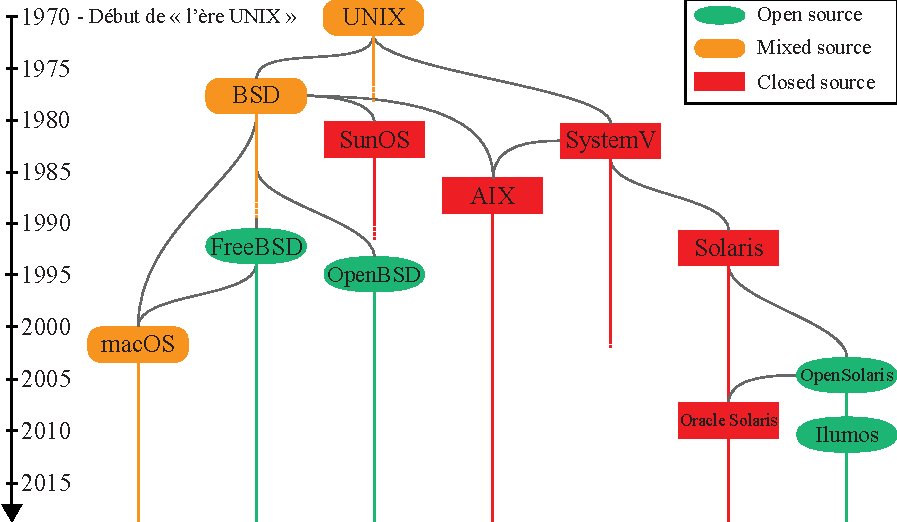
\includegraphics[width=\textwidth]{res/unix_genealogy.pdf}
\centering
\caption{Généalogie simplifiée des systèmes basés sur UNIX}
\label{fig:unix}
\end{figure}

La figure \ref{fig:unix} montre que de nombreux systèmes encore utilisés aujourd'hui sont basés sur UNIX ou ses descendants et qu'il existe de très forts liens entre les différents systèmes, qui s'inspirent et s'influencent mutuellement au cours du temps. Ceci peut souvent être mis en relation avec le fait que certains systèmes ont des sources fermées, ouvertes ou mixtes.

\newpage

\subsubsection{L'héritage d'UNIX}

Bien que UNIX ait été créé à la fin des années 60, on considère que l'ère UNIX ne commence qu'au 1\textsuperscript{er} janvier 1970. Cette date est un repère temporel important pour le monde de l'informatique. D'une part, il s'agit de la date symbolique à partir de laquelle sont apparus les prémices des systèmes actuels. D'autre part, elle est même utilisée comme base de mesure du temps : le nombre de secondes depuis le début de l'ère UNIX se nomme le \textit{timestamp}. Ceci témoigne de l'importance d'UNIX pour l'informatique actuelle.

Un autre aspect de l'importance d'UNIX réside dans les traces qu'il a laissé dans les systèmes d'exploitation, dont certains sont encore fortement utilisés aujourd'hui.

\paragraph{\href{https://www.openbsd.org}{OpenBSD} et \href{https://www.freebsd.org}{FreeBSD}}
Ces deux descendants directs de BSD, créés en 1996 et 1993, sont libres et \textit{open source}, avec un fort accent mis sur la fiabilité du système. OpenBSD est très centré sur la sécurité tandis que FreeBSD, de par sa volonté d'être un système multi-usages, est le système BSD le plus utilisé aujourd'hui. De nombreux éléments de FreeBSD sont d'ailleurs utilisés dans des systèmes dédiés à certains appareils tels que des consoles de jeux (Nintendo Switch, PlayStation 3 et 4\dots).

\paragraph{\href{https://www.ibm.com/power/operating-systems/aix}{AIX}}
Système développé par IBM en 1986, à partir de System V, et inspiré de BSD pour ses serveurs et \textit{mainframes}.

\paragraph{\href{https://www.apple.com/macos}{macOS}}
Anciennement nommé Mac OS X, ce système grand public bien connu et développé par Apple, est fourni gratuitement avec les ordinateurs de son concepteur depuis 2001. Auparavant, Apple distribuait son système propriétaire Macintosh OS depuis 1984. Ce double héritage, issu des différents acquisitions d'Apple, explique qu'une partie des sources sont ouvertes, mais pas libres, tandis que l'autre reste fermée.

\paragraph{\href{http://www.oracle.com/technetwork/server-storage/solaris}{Oracle Solaris}}
Suite à son rachat de Sun, développeur d'OpenSolaris, en 2009 Oracle a décidé de garder ses développements fermés pour créer son propre système propriétaire, dédiés pour ses serveurs.

\paragraph{\href{https://www.illumos.org}{Ilumos}}
Afin de conserver l'aspect open source d'OpenSolaris, la communauté a décidé, en 2010, de créer Ilumos, successeur libre d'OpenSolaris.

En revanche, on notera qu'\textbf{aucun lien hiérarchique entre UNIX et Linux ou GNU n'existe}. Linux et GNU ne sont donc pas des dérivés d'UNIX comme on peut le lire parfois. En revanche, il est indéniable qu'UNIX a influencé la naissance du projet GNU et la conception de Linux.

\newpage

\subsubsection{Le projet GNU}
Parallèlement, le \href{https://www.gnu.org/}{projet GNU} est initié en 1983 par Richard Stallman, qui souhaitait alors \textbf{créer un système d'exploitation complet et libre.} À l'époque, UNIX est assez répandu, mais reste propriétaire, son code source est n'est pas complètement ouvert, ni libre d'utilisation.
Le nom du projet GNU vient directement d'UNIX. Il s'agit d'un acronyme récursif : \textit{GNU's Not UNIX}. En utilisant directement le nom de son concurrent au sein de son projet, Stallman veut montrer la différence qui existe entre les deux systèmes malgré leur similitudes apparentes. C'est en effet en reprenant une partie des concepts d'UNIX, notamment en ce qui concerne son utilisation, que Stallman a construit GNU.

\subsubsection{Logiciel Libre}
Si Richard Stallman a posé ces bases techniques, c'est surtout par la notion de logiciel libre et sa volonté de le répandre et d'en faciliter l'accès qu'il a impacté l'informatique d'aujourd'hui. En effet, qu'il s'agisse de système d'exploitation entier ou de logiciels plus élémentaires, nombreux sont les projets ouverts et libres d'accès, d'utilisation, de partage et de modification.

C'est dans cette optique que Stallman a fondé la \href{https://www.fsf.org}{\textbf{Free Software Foundation}} en 1985, afin de pouvoir gérer les aspects administratifs, juridiques et organisationnels que demandaient le Projet GNU. Ainsi plusieurs licences sont issues de cette fondation, telles que la \href{https://www.gnu.org/licenses/quick-guide-gplv3.html}{\textit{General Public License} (GPL)} ou la \href{https://www.gnu.org/licenses/lgpl-3.0.en.html}{\textit{Lesser Public General License} (LGPL)}, qui sont devenues deux des licences de logiciel libre les plus utilisées. Si un code ou logiciel est distribué sous ces licences, alors toute personne peut est garantie des libertés suivantes : 
\begin{enumerate}
    \item la liberté d’exécuter le programme, pour tous les usages (y compris commercial),
    \item la liberté d’étudier le fonctionnement du programme et de l’adapter à ses besoins,
    \item la liberté de redistribuer des copies du programme,
    \item la liberté d’améliorer le programme et de distribuer ces améliorations au public, pour en faire profiter toute la communauté.
\end{enumerate}
Elle doit cependant toujours notifier les éventuelles modifications du code et laisser ce dernier accessible. De plus, la GPL impose de redistribuer toute modification avec la même licence. On dit alors que GPL est contaminante. Le terme \textit{copyleft}, popularisé par Stallman, est d'ailleurs un jeu de mot utilisé pour décrire la GPL, en opposition au \textit{copyright}.

Il existe de nombreuses autres licences de logiciels libres, créées par des universités ou des fondations impliquées dans le logiciel libre, qui respectent généralement ces libertés, mais précisent d'autres éléments. Le site TLDRLegal\footnote{\textit{Software Licenses in Plain English} - \href{https://tldrlegal.com}{https://tldrlegal.com}} permet de simplifier la compréhension de ces licences.
On pourra citer, notamment : 
\begin{itemize}
    \item \href{https://opensource.org/licenses/MIT}{Licence MIT} (du \textit{Massachusetts Institute of Technology}), qui n'est pas contaminante.
    \item Licences BSD (initiative de \textit{Berkeley Software Distribution}), proches de la licence MIT et établies pour le système BSD. Il en existe plusieurs variantes, toujours non contaminante.
    \item \href{https://www.apache.org/licenses}{Licence Apache}, initiée par la fondation Apache, n'est pas contaminante.
    \item \href{https://www.mozilla.org/en-US/MPL}{Licence Publique Mozilla}, initié par la fondation Mozilla, qui est n'est pas totalement contaminante, mais impose quelques restrictions.
    \item \href{https://creativecommons.org}{Licences \textit{Creative Commons}}, ensemble de licences prédéfinies et simples pour définir les libertés ou restrictions sur une œuvre.
\end{itemize} \vspace{\baselineskip}
\note{Note :} \textbf{Un logiciel peut être \textit{open-source} sans pour autant être considéré comme libre s'il est distribué sans licence ou qu'elle ne donne pas d'autorisations explicites.}

\newpage

\subsection{Généralités sur les systèmes d'exploitation}

\subsubsection{Système d'exploitation}

Un système d'exploitation (\textit{Operating System} ou \textit{OS} en anglais) est ensemble de logiciels permettant à un utilisateur d'exécuter des programmes sur un appareil en liant le matériel et les applications (voir figure \ref{fig:os}). Son rôle principal et de gérer, d'allouer et de protéger les ressources de l'appareil. C'est surtout le noyau (\textit{kernel}) du système qui se charge de ces tâches.

\subsubsection{Noyau}

Le noyau est véritablement le coeur du système d'exploitation. On peut regrouper ses missions en deux catégories : 
\begin{itemize}
    \item Faire l'interface entre le matériel et le logiciel,
    \item Gestion des ressources et des utilisateurs,
    \item Ordonnancement des tâches.
\end{itemize}

C'est donc lui qui permet d'orchestrer l'ensemble du matériel (RAM, clavier, disque dur...). Il permet ainsi à d'autres programmes d'accéder à ces composants et de les utiliser, par une interface unique, qui ne dépend pas du matériel. Les programmes sont ainsi libres d'utiliser le processeur pour effectuer des calculs, l'interface réseau pour contacter d'autres appareil du réseau voire accéder à Internet, ou encore utiliser le disque dur pour stocker des fichiers\dots Le noyau est généralement servi avec toute une série de programmes permettant à l'utilisateur de véritablement utiliser son ordinateur (interface graphique ou en ligne de commande, éditeurs de texte, utilitaires divers, etc.) formant ainsi un système complet et utilisable.

\begin{figure}[hb!]
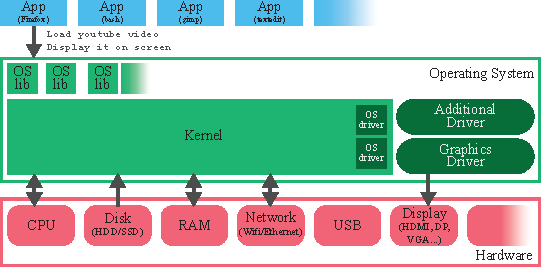
\includegraphics[width=\textwidth]{res/os_architecture.pdf}
\centering
\caption{Exemple de liens entre programmes, OS et matériel}
\label{fig:os}
\end{figure}

Il existe une multitude de systèmes d'exploitation et UNIX fut l'un d'entre eux. Par exemple, Windows, Android, iOS et macOS sont des systèmes d'exploitation. Tous les systèmes d'exploitation sont différents car ils ont été conçus avec des philosophies et contraintes matérielles différentes. C'est pour cela qu'il ne peuvent pas tous être installés sur les mêmes appareils et qu'ils s'utilisent différemment.

\newpage

\subsection{Les systèmes GNU/Linux} \vspace{-4mm}

\textbf{GNU/Linux est un ensemble de logiciels, issu du projet GNU, formant un système d'exploitation complet, libre et ouvert.} Linux, à lui seul, n'est pas un système d'exploitation à part entière puisqu'il s'agit d'un noyau. Le développement du noyau Linux a été initié par Linus Torvalds en 1991. Aujourd'hui, de très nombreux appareils (ordinateurs, serveurs, routeurs WiFi, consoles de jeu, téléphones\dots) utilisent un noyau Linux, ce qui rend les systèmes GNU/Linux majoritaires sur le marché des systèmes d'exploitation.

Ainsi, bien que UNIX soit un ancêtre commun à une multitude de systèmes d'exploitation encore utilisés aujourd'hui, \textbf{GNU/Linux en est totalement indépendant}. Richard Stallman et Linus Torvalds ont probablement été influencés par UNIX, mais GNU/Linux a été créé de zéro et n'est donc pas un dérivé d'UNIX, et ne figure pas sur la généalogie d'UNIX.

De plus, une autre fonctionnalité centrale aux distributions Linux est le système de paquets. Chaque programme est disponible sous forme de paquet, chaque paquet pouvant avoir des dépendances vers d'autres paquets. L'ensemble des paquets est disponible sur des serveurs proposant une interface commune à l'acquisition de programmes.

Il existe plusieurs systèmes utilisant un noyau Linux. La plupart sont regroupés sous le terme de \say{Distribution Linux}, puisque de nombreux logiciels sont distribués conjointement, en plus du noyau et des outils basiques formant le système GNU/Linux. Et, de la même manière que pour la généalogie d'UNIX, de très nombreuses distributions GNU/Linux existent et s'influencent les unes des autres, comme l'illustre la figure \ref{fig:distrib}.
\vspace{-2mm}
\begin{figure}[hb!]
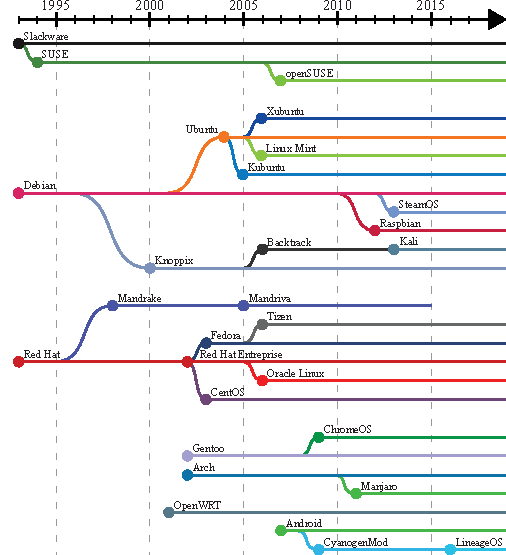
\includegraphics[width=0.70\textwidth]{res/linux_distrib_genealogy_links.pdf}
\centering
\vspace{-1mm}\caption{Généalogie simplifiée des principaux systèmes utilisant un noyau Linux}\label{fig:distrib}
\vspace{-\baselineskip}
\end{figure}

\newpage

\paragraph{Distributions basées sur Debian}

Il existe de nombreuses distributions basées sur \href{https://www.debian.org}{Debian}. Il s'agit d'une des distributions les plus anciennes, qui est la seule qui ne soit pas gérée par une entreprise. Debian met en avant la stabilité de son système, ce qui en a fait le favori des serveurs. Il existe plusieurs versions maintenue en parallèle, afin d'équilibrer entre stabilité et nouvelles fonctionnalités.

La variante la plus connue de Debian est \href{https://www.ubuntu.com}{Ubuntu}. Elle été créée afin de faciliter l'utilisation de Linux par le grand public. Elle dispose de plusieurs variantes (\href{https://kubuntu.org}{Kubuntu}, \href{https://xubuntu.org}{Xubuntu} ou \href{https://lubuntu.net/}{Lubuntu}) qui proposent un gestionnaire de bureau et des applications différentes, ainsi que d'autres variantes dédiées à des utilisations particulières. Il existe également des versions d'Ubuntu dédiée pour les téléphones : Ubuntu Touch. Le projet a été abandonné par Canonical mais repris par des développeurs indépendants.

\href{https://www.raspberrypi.org/downloads/raspbian/}{Raspbian} est une variante de Debian dédiée aux mini-ordinateurs Raspberry Pi. Elle est optimisée pour être exécutée sur ce système aux performances restreintes.

Les distributions basées sur Debian utilisent le système de paquets éponyme, avec les utilitaires \texttt{dpkg}\command{dpkg} pour gérer les paquets \texttt{.deb}, et \texttt{apt}\command{apt} pour gérer les dépendances et mises-à-jour de paquets.

\paragraph{Distributions basées sur Red Hat}

Red Hat (Entreprise Linux) est une des plus anciennes distribution, et est maintenue par l'entreprise du même nom.

Mandriva a été maintenue par une équipe française et se voulait simple d'utilisation. Elle est, depuis peu, reprise par la communauté sous le nom \href{https://www.openmandriva.org}{OpenMandriva}.

\href{https://www.centos.org}{CentOS} est le pendant libre de  \href{https://www.redhat.com/en/technologies/linux-platforms/enterprise-linux}{Red Hat Entreprise Linux} (RHEL). Dédiée aux serveurs, c'est une des distributions Linux les plus utilisées.

\href{https://getfedora.org/}{Fedora} est une autre distribution basée sur Red Hat. Elle propose des programmes libres et sous d'autres licences. Les nouveautés intégrées dans Fedora le sont a \textit{posteriori} dans Red Hat, ce qui en fait une des distributions les plus actualisées.
Les distributions basées sur Debian utilisent le système de paquets \textit{RPM} pour \textit{RPM Package Manager} (Anciennement \textit{Redhat Package Manager}. Le programme \texttt{yum}\command{yum} permet de gérer les paquets et leurs dépendances. Il a été remplacé par \texttt{dnf}\command{dnf} dans Fedora.

\paragraph{Distributions indépendantes}

\href{https://www.gentoo.org}{Gentoo} a été créé avec la conception que chaque programme doit être compilé avant d'être installé, ce qui permet de personnaliser l'installation et surtout d'optimiser la compilation pour le type d'ordinateur, permettant des performances légèrement meilleures.

\href{https://www.archlinux.org}{Arch Linux} est un système minimaliste, encourageant une forte implication de sa communauté. Ainsi, une installation Arch Linux est très légère car ne distribue que très peu de programmes supplémentaires. La prise en main s'en retrouve en revanche plus longue. Arch Linux dispose de son propre gestionnaire de paquets,\texttt{pacman}, et d'une documentation extrêmement complète et détaillée. Il existe une variante qui se veut facile à prendre en main : \href{https://manjaro.org}{Manjaro}.

\href{https://openwrt.org}{OpenWRT} est un système dédié pour les routeur WiFi et allégé de tous les composants non nécessaires pour cet usage particulier.

\href{https://www.android.com}{Android}, bien qu'il ne soit pas considéré à proprement parler comme une distribution Linux, est un système d'exploitation au noyau Linux, développé par Google. Il existe une variante principale, CyanogenMod, devenue \href{https://lineageos.org}{LineageOS}, qui est gérée par des développeurs indépendants.

\newpage

\subsection{Interfaces de contrôle}\vspace{-4mm}

Quel que soit le système d'exploitation, il dispose toujours d'une interface de contrôle (voir figure \ref{fig:interface}. Celle-ci peut être graphique ou en console. Dans le second cas, on parle aussi de lignes de commandes, d'émulateur de terminal ou de terminal voire, en anglais, de \textit{CLI} pour \textit{Command Line Interface} et plus souvent de TTY (pour \textit{TeleTYpewriter}). L'interface graphique d'un système est gérée par un gestionnaire de bureau (\textit{desktop manager}), qui va afficher et présenter les différents programmes en cours d'exécution, et permettre à l'utilisateur de les gérer.

Le mode graphique varie grandement entre les systèmes d'exploitation. Sous iOS, macOS et Windows, il n'existe qu'un seul gestionnaire de bureau. Sous GNU/Linux, celui-ci est totalement optionnel. Il existe une multitude de gestionnaires de bureau pour GNU/Linux, qui reposent sur différentes philosophies. C'est d'ailleurs souvent pour proposer un gestionnaire de bureau spécifique que des distributions Linux sont créées.

Tous ces environnements sont cependant basés sur une couche logicielle standardisée, qui se nomme \href{https://www.x.org}{X}. En 2008, une nouvelle couche d'affichage graphique, \href{https://wayland.freedesktop.org}{Wayland}, a fait son apparition et il est supporté et utilisé par de plus en plus de gestionnaires de bureau.

Il est possible d'utiliser une interface en ligne de commande à partir d'une interface graphique et cela permet notamment d'utiliser la souris ou le \textit{multitasking} (utilisation de plusieurs applications simultanément) via l'utilisation de fenêtres pour les programmes. Mais lorsqu'aucun gestionnaire de bureau n'est installé, la ligne de commande pure (sans fenêtre, ni souris, uniquement du texte) est incontournable.

Enfin, l'interface en ligne de commande permet souvent un contrôle rapide et fin de ce que l'on souhaite faire, puisqu'aucune surcouche ne masque ce qui est réellement exécuté. L'interface en ligne de commande permet donc de mieux comprendre ce que l'on fait, ainsi que le fonctionnement du système. Elle nécessite en revanche un apprentissage plus long et moins instinctif qu'une interface graphique interactive.

\begin{figure}[hb!]
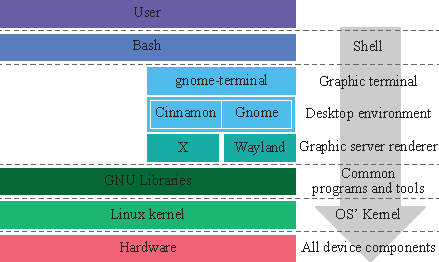
\includegraphics[width=0.78\textwidth]{res/linux_control_interface.pdf}
\centering
\caption{Schéma des couches de contrôle d'un système GNU/Linux}
\label{fig:interface}
\end{figure} \vspace{-2mm}

\note{Note :} Dans la figure \ref{fig:interface}, on peut remarquer que la couche graphique est totalement optionnelle pour utiliser le système et que les environnements de bureau restent indépendants du serveur graphique.

\newpage

\subsection{Arborescence de fichiers} \label{sec:directories}
Un fichier est une zone sur le disque dur pouvant contenir des données. Cette zone est définie par un début et une taille. Cette taille peut évoluer au court du temps, en fonction des actions sur le fichier. Chaque fichier est placé dans un dossier qui peut regrouper plusieurs fichiers et dossiers, formant ainsi une arborescence. Ainsi, un fichier est identifié par son chemin, c'est-à-dire les dossiers successifs qui le contiennent, et son nom. Un chemin de fichier est toujours unique. Pour gérer cette arborescence, le système d'exploitation utilise un système de fichiers qui répertorie les fichiers et gère les accès et modifications sur le disque par l'utilisateur.

Une des philosophie de Linux est que \textbf{\say{tout est fichier}}. Ainsi, tout est représenté sous forme de fichiers, y compris les dossiers, qui sont considérés comme des fichiers particuliers. Les systèmes Linux ont une architecture particulière et universelle. Tous les dossiers sont (directement ou indirectement) dans le dossier racine (\textit{root}), que l'on représente par un \textit{slash} (\texttt{/}), comme illustré dans la figure \ref{fig:linux_tree}. On notera que '\texttt{/}' est à la fois le nom du dossier racine, mais également le séparateur des dossiers.

\subsubsection{Chemin de fichiers}

Chaque fichier est accessible par un chemin de fichier, qui peut être absolu ou relatif. Un chemin de fichier est une suite de nom de dossiers séparés par des \textit{slash}.

\paragraph{Chemin absolu}

\textbf{Un chemin absolu est un chemin qui commence par la racine}, il commence donc par un '\texttt{/}'. Par exemple, pour identifier le dossier \texttt{usr1} dans le dossier \texttt{home} de la racine, on aura le chemin absolu \texttt{/home/usr1}.

\paragraph{Chemin relatif}

Un chemin relatif est un chemin relatif au dossier courant. Pour le même dossier que précédemment, si on se trouve dans le dossier \texttt{/home}, alors le chemin relatif sera \texttt{usr1}, tandis que si on se trouve dans la racine, il sera \texttt{home/usr1}.

Ajouté à cela, il existe deux dossiers spéciaux (ou relatifs), présents dans tous les dossiers et utilisables au sein des chemins absolus et relatifs : 
\begin{itemize}
    \item \texttt{.} (point) : il représente le dossier courant,
    \item \texttt{..} (point point) : il représente le dossier parent.
\end{itemize}

Ainsi, si l'on se trouve dans le dossier \texttt{/bin}, le chemin relatif vers le dossier \texttt{/home/usr1} sera \texttt{../home/usr1}.

\note{Note :} Bien qu'un chemin absolu puisse utiliser les dossiers '\texttt{.}' et '\texttt{..}' en restant absolu, le chemin en est rallongé (il contient plus de dossier). On dit qu'\textbf{un chemin absolu est canonique lorsqu'il ne contient aucun dossier relatif}.

\paragraph{Dossier personnel}

De plus, il existe un autre caractère spécial, que l'on a déjà évoqué : \texttt{\tilde}. Il ne s'agit pas d'un véritable dossier, mais d'un alias ou raccourci vers le dossier personnel (ou \hyperref[sec:dirhome]{\texttt{home}}) de l'utilisateur courant. De plus \texttt{\tilde user} représente le dossier personnel de l'utilisateur \texttt{user}.

Enfin, \textbf{les fichiers dont le nom commence par '\texttt{.}' sont des fichiers cachés} : ils ne sont pas visibles par défaut. On les trouve notamment dans le dossier personnel de chaque utilisateur, ils contiennent généralement des configurations ou cache de différentes applications. Les dossiers \texttt{.} et \texttt{..} sont donc des dossiers cachés.

\newpage
\subsubsection{Architecture des dossiers Linux}

\begin{figure}[hb!]
    \centering
\begin{forest}
  my label/.style={
    label={[font=\sffamily]right:{#1}},
  },
  for tree={
    text=white,
    minimum height=0.75cm,
    font=\footnotesize\ttfamily,
    if level=0{fill=dirblue2}{fill/.wrap pgfmath arg={dirblue#1}{int(4-(mod((level()-1),4)))}},
    if level=1{l=20mm}{l=15mm},
    rounded corners=4pt,
    edge={gray,rounded corners,line width=0.5pt},
    child anchor=north,
    parent anchor=south,
  },
[/
  [bin]
  [boot
    [grub]
  ]
  [dev]
  [etc
    [apt]
    [init.d]
    [X11]
  ]
  [home
    [1A]
    [depot]
    [\dots]
  ]
  [lib]
  [mnt
    [usb]
  ]
  [root]
  [tmp]
  [usr
    [bin]
    [lib]
  ]
  [var]
]
\end{forest}
    \caption{Extrait de l'arborescence commune aux différents systèmes Linux}
    \label{fig:linux_tree}
\end{figure}


\textbf{Descriptif du contenu chaque dossier majeur}

\begin{tabularx}{\textwidth}{| c | X |}  \hline
    \texttt{/bin}                    & Fichiers exécutables (\textbf{bin}aires) pour l'initialisation du système et les commandes \say{essentielles} pour sa gestion \\
        \hline
    \texttt{/boot}                   & Le noyau dans ses différentes versions installées ainsi que les fichiers de démarrage : \newline
            --~\texttt{grub} : Chargeur d'amorçage, utilitaire pour détecter les systèmes d'exploitation disponibles. \href{https://www.gnu.org/software/grub/}{GRUB} permet de choisir l'OS et le mode de démarrage. \\
        \hline
    \texttt{/dev}\label{sec:dirdev}  & Fichiers spéciaux représentant les composants ou appareils (\textit{\textbf{dev}ices}) détecté par le système (disques durs, lecteurs Blu-ray, interfaces réseau\dots). \newline
            On y trouve également \texttt{null}, \texttt{zero} et \texttt{random} (voir partie \ref{sec:file_dev}). \\
        \hline
    \texttt{/etc}                     & Fichiers de configuration du système et de diverses applications : \newline
            --~\texttt{apt} : configuration du gestionnaire de paquet Aptitude, \newline
            --~\texttt{rc.d} : scripts de démarrage du système, \newline
            --~\texttt{X11} : configuration du serveur d'affichage X. \\
        \hline
    \texttt{/home}\label{sec:dirhome} & Contient les dossiers personnels des utilisateurs. \newline À TELECOM Nancy, ce dossier est en réalité un dossier réseau contenant les dossiers des enseignants et des élèves : \newline
            --~\texttt{1A}, \texttt{2A}, \texttt{3A} : contient les dossiers personnels des élèves de l'année correspondante, \newline
            --~\texttt{EqPedag} : contient les dossiers personnels des enseignants, \newline
            --~\texttt{depot} : dossier commun pour les TP. \\
        \hline
    \texttt{/lib} & Bibliothèques et modules noyau. \\
        \hline
    \texttt{/media}                   & Dossier des fichiers contenus sur clés USB et disques externes connectés (supports amovibles). Est parfois absent ou confondu avec \texttt{/mnt}. \\
        \hline
    \texttt{/mnt}                     & Dossier des fichiers contenus périphériques internes (disques dur, lecteurs Blu-ray\dots). On dit de ces dossiers qu'ils sont des points de montage des partitions ou appareils (\textit{\textbf{m}ou\textbf{nt}} en Anglais). \\
        \hline
    \texttt{/opt}                     & Dossier d'installation des applications supplémentaires \textbf{opt}ionelles. \\
        \hline
    \texttt{/proc}                    & \say{Image} du système avec des informations sur le \textbf{proc}esseur, la RAM\dots \\
        \hline
    \texttt{/root}                    & Dossier personnel du super-utilisateur (nommé \textit{\textbf{root}}) (voir partie \ref{cmd:sudo}). \\
        \hline
    \texttt{/sbin}                    & Fichiers exécutable pour l'administration du système : gestion du disque, des interfaces réseau, des différents services\dots \\
        \hline
    \texttt{/tmp} & Fichiers \textbf{t}e\textbf{mp}oraires. \\
        \hline
    \texttt{/usr}                     & Programmes accessibles à tous les utilisateurs (\textit{\textbf{us}e\textbf{r}}). Ce dossier possède une structure semblable à la racine. \\
        \hline
    \texttt{/var}                     & Données \textbf{var}iables liées à la machine et notamment des fichiers journaux, archivant les événements du systèmes dans \texttt{/var/log}. \\
        \hline
\end{tabularx}

\newpage
\newpage


%%%%%%%%%%%%%%%%%%%%%%%%%%%%%%%
\section{Manipulation d'un système GNU/Linux}
Dans cette partie et les parties suivantes, on considère que l'on dispose d'un système GNU/Linux avec l'interpréteur de commande Bash. Sauf mention contraire, l'ensemble des exemples et commandes devraient fonctionner sans problèmes sous toutes les distributions GNU/Linux, sous macOS et même avec le \href{https://docs.microsoft.com/fr-fr/windows/wsl/install-win10}{sous-système Linux sur Windows} (\textit{Windows sub-system for Linux}, WSL), à condition d'utiliser Bash.

\note{Note:} On parlera de \say{terminal} ou de \say{console} pour l'interface en ligne de commande (ou de \say{CLI}, pour \textit{Command Line Interface}), mais de \say{Shell} pour parler du programme sous-jacent permettant l'interprétation des commandes (Bash).

\vspace{-3mm}
\subsection{POSIX} \label{sec:POSIX}
\vspace{-3mm}
Si l'ensemble des outils GNU/Linux sont similaires sur tous les systèmes et dérivés d'UNIX, ce n'est pas un hasard. Devant la multiplication des variantes d'UNIX, \textbf{les standards POSIX (pour \textit{Portable Operating System Interface}) ont été établis en 1988} pour proposer une \textbf{interface d'utilisation commune à tous les systèmes UNIX}.

La majeure partie des commandes et des programmes présentés ci-après respectent les dernières versions de  POSIX et peuvent donc être utilisés comme indiqué sur tous les systèmes qui les proposent. \textbf{Il existe cependant quelques rares cas dans lesquels le standard n'est pas respecté} (pour des raisons philosophiques ou historiques), mais ils sont explicités au sein de leur documentation.

\subsection{Ligne de commande}

\subsubsection{Usages et intérêt}

Bien que la plupart des systèmes de bureau disposent d'une interface graphique, la gestion quotidienne du système peut se faire intégralement en ligne de commande. De nombreux programmes ne sont d'ailleurs qu'une surcouche à leur version console, pour plus de simplicité.

De manière générale, la ligne de commande permet à un utilisateur de se connecter, d'exécuter des programmes et d'interagir le système. Utiliser la ligne de commande permet également d'agir de façon plus uniforme, grâce à POSIX (voire partie \ref{sec:POSIX}).

\subsubsection{Plusieurs terminaux}
Il existe deux types de terminaux : 
\begin{itemize}
    \item Graphique (tel que \texttt{gnome-terminal}), permettant d'utiliser un terminal graphique,
    \item Terminal pur, ne permettant d'afficher que du texte.
\end{itemize}
\vspace{\baselineskip}

Il existe plusieurs terminaux, identifié par un numéro, et accessible grâce au raccourci clavier \texttt{Ctrl+Alt+<FX>}. \textbf{Par défaut, l'interface graphique s'exécute dans un terminal}, généralement le TTY7 ou le TTY1. Ainsi, le raccourci clavier \texttt{Ctrl+Alt+F2} permet de passer au TTY2 à tout moment, passant en mode terminal pur, si celui-ci existe bien.

\newpage

\subsection{Prise en main du terminal}
\vspace{-4mm}
Lorsque l'on lance un terminal, il n'y a généralement aucun affichage, seuls quelques caractères s'affichent au début de ligne. Il s'agit de l'invite de commande ou \textit{prompt}.
\subsubsection{Invite de commande -- \textit{prompt}}

Le \textit{prompt}, lorsqu'il n'est pas personnalisé\footnote{Le prompt peut-être personnalisé par la variable d'environnement (voir partie \ref{sec:env}) \texttt{PS1}. La syntaxe pouvant être complexe, des générateurs en ligne existent comme \href{http://ezprompt.net}{ESPrompt} ou \href{http://bashrcgenerator.com}{.bashrc generator}}, est généralement de la forme suivante :
\begin{nscenter}
    \texttt{login@machine:\tilde~\$}
\end{nscenter}

Si on l'analyse, peut détailler trois parties :
\begin{itemize}
    \item \texttt{login@machine}, identifie l'utilisateur courant (via son login) et la machine courante (via son nom). Cela peut paraître superflu au premier abord mais s'avère très utile lorsque l'on se connecte à plusieurs machines à distance (voir partie \ref{cmd:ssh}).
    \item \texttt{\tilde}, correspond au dossier courant. En l'occurrence, il s'agit d'un alias qui correspond au dossier personnel de l'utilisateur courant (voir partie \ref{sec:dirhome}). En changeant de dossier, cette valeur changera pour le nom ou le chemin du nouveau dossier.
    \item \texttt{\$}, correspond au niveau d'utilisateur. \texttt{\$} signifie utilisateur normal, \texttt{\#} signifie super-utilisateur. L'utilisateur normal peut, le temps d'une commande, acquérir les droits de super-utilisateur (voir partie \ref{cmd:sudo}), sans que ce symbole change.
\end{itemize}\vspace{1mm}

Lorsque le \textit{prompt} est affiché, cela signifie que l'on peut entrer une commande.

\subsubsection{Structure d'une commande} \label{sec:command}

Une commande, quel que soit le système d'exploitation, est une chaîne de caractère que l'on va taper au clavier pour réaliser une action sur le système. Elle se compose de plusieurs mots ou codes, \textbf{les arguments}, séparés par au moins un espace. On représente une commande ainsi :
\begin{nscenter}
    \mintinline{bash}{command [ --long-option | -o -p <value> -t ] parameter}
\end{nscenter}
\begin{itemize}
    \item \texttt{command} - La commande est presque toujours en minuscule, parfois composés de plusieurs mots, séparés par des tirets (\texttt{-}) ou des sous-tirets (\texttt{\_}) ;
    \item Les arguments entre crochets (\texttt{[]}) sont facultatifs, ce sont des options ;
    \item les arguments séparés par des \textit{pipes} (\texttt{|}) indiquent une alternative : ils sont exclusifs et ne peuvent être utilisés simultanément ;
    \item les argument entre chevrons (\texttt{<>}) sont à remplacer par le texte voulu. Ils ne sont pas toujours entre chevrons mais différencié des autres arguments (majuscules, couleurs\dots)
\end{itemize}
\note{Note :} On présente souvent une commande ou une séries de commandes, en précédant la ou les lignes par le symbole de niveau d'utilisateur, qui ne fait alors pas partie de la commande.

\paragraph{Notation des arguments d'options}

Il existe deux types d'arguments d'options : les arguments courts et les arguments longs.
\begin{itemize}
    \item Les arguments courts commencent par un tiret et ne comportent qu'une seule lettre (voir chiffre, dans de très rares cas), majuscule ou minuscule. Ils peuvent nécessiter une valeur, qui est alors précisée par le paramètre suivant : \mintinline{bash}{command -o -p -t value}.\newline
    Il est possible de combiner les paramètres courts pour plus de simplicité : \mintinline{bash}{command -opt}\vspace{\baselineskip}
    
    \item Les arguments longs commencent par un double tiret et comportent généralement un mot complet ou plusieurs mots séparés par des tirets (\texttt{-}) ou des sous-tirets (\texttt{\_}). Leur valeur peut aussi être donnée via un signe égal (\texttt{=}): \mintinline{bash}{command --option value --long-option=true}
\end{itemize}
\newpage

Les arguments de chaque commande sont explicités dans le manuel. Pour consulter le manuel d'une commande, il suffira d'utiliser la commande \texttt{\cmdref{man} <command>} (voir partie \ref{cmd:man}).

\warning{Enfin, une commande dispose toujours (même s'ils ne sont pas utilisés):}
\begin{itemize}
    \item D'un code de retour (ou code d'erreur) (voir partie \ref{sec:error}),
    \item D'une entrée sur laquelle elle peut lire des données (voir partie \ref{sec:redirect}),
    \item D'une sortie sur laquelle elle peut écrire des données (voir partie \ref{sec:redirect}),
    \item D'une sortie d'erreur, dédiée au messages d'erreur (voir partie \ref{sec:redirect}).
\end{itemize}

\subsubsection{Premières commandes}

Les premières commandes essentielles à apprendre permettent d'obtenir des informations sur la sessions courante ou le système. Elles sont détaillées dans le tableau \ref{tab:first_cmd}.
\begin{table}[bh!]
    \centering
    \begin{tabularx}{\textwidth}{| c | X |}  \hline
        \textbf{Commande} & \textbf{Description}                                                                                                \\ \hline
        \texttt{whoami} \command{whoami}  & Affiche le login de l'utilisateur courant.                                                          \\ \hline
        \texttt{pwd} \command{pwd}        & Affiche le dossier courant (\textit{PoWer Directory}). Plus de détails partie \ref{sec:directories}.\\ \hline
        \texttt{echo} \command{echo}      & Affiche le message passé en premier paramètre. Avec \texttt{-n}, pas de saut de ligne.              \\ \hline
        \texttt{apropos} \command{apropos}& Recherche les commandes relatives au mot-clé passé en premier paramètre.                            \\ \hline
        \texttt{history} \command{history}& Affiche les commandes récentes (le nombre est passé en paramètre).                                  \\ \hline
        \cmdref{man}                      & Affiche le manuel d'utilisation de la commande passée en paramètre.                                 \\ \hline
        \texttt{info} \command{info}      & Alternative à \cmdref{man} proposée par GNU, basée sur des sections navigables.                        \\ \hline
        \texttt{help} \command{help}      & Affiche l'aide pour les commandes internes de Bash sans page de manuel.                             \\ \hline
    \end{tabularx}
    \caption{Commandes basiques permettant d'obtenir des informations sur le système.}
    \label{tab:first_cmd}
\end{table}
\vspace{-4mm}

Hormis quelques rares exceptions, les commandes sont toutes des programmes. Cela signifie qu'un exécutable est présent sur le système et est appelé lorsque l'on valide la commande. Ce fonctionnement est possible grâce à la variable d'environnement \texttt{\$PATH}, détaillée partie \ref{sec:env}.

\subsubsection{À propos du manuel -- \texttt{man}} \command{man}

Le manuel regroupe la documentation de toutes les commandes installées sur le système. Il existe plusieurs sections de manuel, allant de 1 à 9. Ces sections sont décrites dans le manuel de la commande \cmdref{man}, consultable grâce à la commande \mintinline{bash}{man man}. On notera que la section \texttt{1} contient les pages de manuel des commandes Bash. Dans le cas ou une page de manuel a des homonymes dans d'autres sections, on peut forcer la section \texttt{X} : \mintinline{bash}{man X command}

La plupart des pages de manuel comportent une présentation succincte de la commande (le synopsis) ainsi qu'une description de la commande, de ses cas d'usages et de ses paramètres. Il y a généralement une partie définissant les codes de retour possibles et leur signification. Certaines pages on également des exemples d'utilisations et de résultats attendus.

En général, lorsqu'on utilise le manuel, on dispose d'une interface dédiée. On peut naviguer dans le manuel avec les flèches directionnelles et les touches \texttt{PageUp} et \texttt{PageDown}. Pour effectuer une recherche, on tapera un \textit{slash} (\texttt{/}) suivi du mot clé à rechercher, puis \texttt{Entrée}. \texttt{N} passera à la prochaine occurrence et \texttt{P} à l'occurrence précédente. \texttt{Q} permet de quitter.

Il se peut cependant que certaines commandes ne bénéficient pas de page de manuel ni d'aide. Dans ce cas, on peut essayer d'appeler la commande avec l'option \texttt{--help} ou \texttt{-h}. Cette option affiche généralement comment utiliser la commande et les arguments qu'elle peut prendre.

\newpage

\vspace{-4mm}
\subsubsection{Raccourcis de saisie}
\vspace{-2mm}

Le terminal étant conçu pour être utilisé intégralement au clavier, il existe de nombreux raccourci pour faciliter la saisie et le déplacement du curseur. Des éléments plus précis sur la notation des raccourcis clavier figurent en annexe \ref{appendix:shortcuts}.

\begin{table}[h!]
    \centering
    \begin{tabularx}{\textwidth}{| c | X |}  \hline
        \textbf{Raccourci} & \textbf{Effet} \\ \hline
        \texttt{Tab}      & Auto-complète le nom de commande courant ou le chemin si possible. \newline                                                                                                  Appuyer deux fois de suite pour voir la liste des suggestions. \\  \hline
        \texttt{\textuparrow} \scriptsize{(flèche haut)}    & Affiche la commande précédente dans l'historique. \\  \hline
        \texttt{\textdownarrow} \scriptsize{(flèche bas)}   & Affiche la commande suivante dans l'historique. \\  \hline
        \texttt{Ctrl + L} & Nettoie l'écran de tout affichage. Sous macOS, nettoie jusqu'à la commande précédente. \\  \hline
        \texttt{Ctrl + C}                                   & Interrompt l'exécution de la commande en cours. \\  \hline
        \texttt{Ctrl + Z} & Mets la commande en cours d'exécution en pause, pour la reprendre plus tard. \newline                                                                                                       Voir partie \ref{sec:tasks}. \\  \hline
        \texttt{Ctrl + D} & Interrompt la saisie lorsqu'une commande en attend une.  \newline                                                                                                                           Permet aussi de quitter le Shell. \\  \hline
        \texttt{Ctrl + \textleftarrow}                      & Déplace le curseur au mot précédent. Équivalent à \texttt{Alt+B}. \\  \hline
        \texttt{Ctrl + \textrightarrow}                     & Déplace le curseur au mot suivant. Équivalent à \texttt{Alt+F}.\\  \hline
        \texttt{Ctrl + R} & Recherche dans l'historique des commandes en tapant quelques caractères. \newline
                            Retaper le raccourci pour passer à la commande correspondante précédente. \\  \hline
        \texttt{Ctrl + S}                                   & Pause le défilement d'affichage de la commande en cours d'exécution. \\  \hline
        \texttt{Ctrl + Q}                                   & Reprend l'exécution de la commande mise en pause par \texttt{Ctrl + S}. \\  \hline
    \end{tabularx}
    \caption{Principaux raccourcis clavier dans un terminal Linux}
    \label{tab:kbd_shortcuts}
\end{table}

De plus, les flèches de déplacement traditionnelles sont bien évidemment utilisables. On notera tout de même les touches suivantes : 
\begin{itemize}
    \item \texttt{Home} ou \texttt{Début} ou \texttt{$\nwarrow$}, qui permet de revenir au début de la commande ou de la ligne.
    \item \texttt{End} ou \texttt{Fin}, qui permet d'aller à la fin de la commande ou de la ligne.
\end{itemize}

\medskip

Enfin, la souris peut être utile si l'on dispose d'un environnement graphique : 
\begin{table}[h!]
    \centering
    \begin{tabularx}{\textwidth}{| c | X |}  \hline
        \textbf{Raccourci souris}   &   \textbf{Effet} \\ \hline
        \texttt{Clic gauche}        &   Sélectionne le texte et le copie. \\  \hline
        \texttt{Clic droit}         &   Colle le texte copié \warning{OU} affiche le menu contextuel. \\  \hline
        \texttt{Clic molette}       &   Colle le texte copié. \\  \hline
    \end{tabularx}
    \caption{Principaux raccourcis souris dans un terminal Linux graphique}
    \label{tab:mouse_shortcuts}
\end{table}
\vspace{-7mm}

\note{Note :} Ces raccourcis peuvent varier légèrement en fonction du système ou de l'interface utilisée. Les raccourcis de déplacement du curseur sont généralement utilisables au sein de l'ensemble des éditeurs de texte.

\paragraph{Rappeler la dernière commande}
Il est possible d'utiliser deux points d'exclamation (\texttt{!!}) pour réutiliser la dernière commande. On peut la compléter et la combiner avec n'importe quelle autre commande. Ce raccourci est notamment utilisé pour rappeler la dernière commande avec les droits du super-utilisateur : \texttt{sudo !!} (voir partie \ref{sec:su}).
%Une variante existe permettant d'appeler la dernière instance d'une commande donnée : \texttt{!command}.

\newpage
\subsection{Système de fichier}
\vspace{-2mm}
%Plusieurs commandes sont disponibles pour pouvoir afficher, se déplacer et manipuler l'arborescence de fichiers détaillée dans la partie \ref{sec:directories}).

\subsubsection{Commandes de manipulation}

\paragraph{\texttt{ls}} \command{ls}
\textbf{L}i\textbf{s}te un dossier dont le chemin le chemin (absolu ou relatif) est passé en paramètre. Sans paramètre, elle affichera le contenu du dossier courant. Lorsque le chemin donné est celui d'un fichier qui n'est pas un dossier, il est listé seul. \newline
\cmdref{ls} dispose de plusieurs options : 
\begin{itemize}
    \item \texttt{-a} : Affiche tous les fichiers, y compris les fichiers cachés. 
    \item \texttt{-H} : En combinaison avec \texttt{-l}, affiche la taille des fichiers en multiples de 1024 octets plutôt qu'en octets. On parle de taille lisible par l'\textbf{h}umain.
    \item \texttt{-l} : Affiche les informations détaillées.
    Dans ce mode, plusieurs informations sont détaillées, avec uniquement un fichier par ligne. Chaque élément de ligne contient différentes informations (voir figure \ref{fig:lsl}). Le type est détaillé dans la partie \ref{sec:filetypes}, les droits d'usages sont détaillés dans la partie dédiée à \cmdref{chmod}, la notion de propriétaires est détaillée dans la partie \ref{sec:users}.
\end{itemize}

\begin{figure}[h!]
        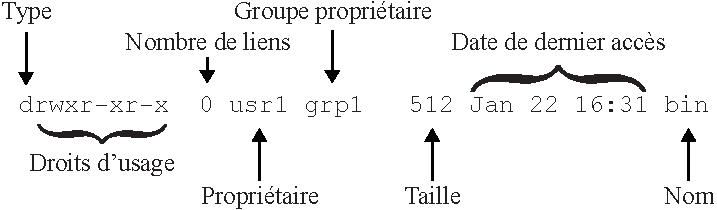
\includegraphics{res/lsl.pdf}
        \centering
        \caption{Détail de l'affichage détaillé de \texttt{ls}.}
    \label{fig:lsl}
\end{figure}

\paragraph{\texttt{cd}} \command{cd}
Permet de se déplacer vers le dossier dont le chemin (absolu ou relatif) est passé en paramètre. Si aucun paramètre n'est donné, retourne au dossier personnel (\texttt{\tilde}).
\begin{itemize}
    \item \texttt{-} : Retourne au dossier précédent. Un second appel à \mintinline{bash}{cd -} retourne au premier dossier car il n'y a pas d'historique.
\end{itemize}
\vspace{3mm}

\note{Note :} Les commandes \texttt{pushd}\command{pushd} et \texttt{popd}\command{popd} permettent de gérer un historique des dossiers sous forme de pile, permettant ainsi de faciliter le retour aux dossiers précédents. \newline 
De plus, le programme \texttt{ranger}\command{ranger} (non installé par défaut) permet un affichage et une navigation plus visuelle, mais ne peut pas être utilisé dans un script.

\paragraph{\texttt{mkdir}} \command{mkdir}
Créé les dossiers passés en paramètres. Il peut s'agir de chemins complets (relatifs ou absolus) ou juste de noms de dossiers à créer.
\begin{itemize}
    \item \texttt{-p} : Créé tous les dossiers parents nécessaires et ne renvoie pas d'erreur si le dossier existe.
    \item \texttt{-m <perm>} : Créé le dossier avec les droits d'accès donnés, à la manière de \cmdref{chmod} (voir partie \ref{sec:chmod}).
\end{itemize}

\paragraph{\texttt{rm}} \command{rm}
Supprime les fichiers ou dossiers passés en paramètres.
\begin{itemize}
    \item \texttt{-i} : Mode interactif. Demande confirmation avant suppression de chaque éléments.
    \item \texttt{-f} : Mode forcé. Suppression du fichier sans confirmation.
    \item \texttt{-r} : Mode récursif. Supprime récursivement un dossier et tous ses sous-dossiers.
\end{itemize}
\vspace{3mm}

\note{Note :} La commande \texttt{rmdir}\command{rmdir} permet de supprimer un ou plusieurs dossiers vides.

\newpage

\paragraph{\texttt{cp}} \command{cp}
Copie les fichiers ou dossiers passés en paramètres vers le dernier paramètre. Si plusieurs fichiers sont à copiés, le dernier paramètre doit être un dossier.
\begin{itemize}
    \item \texttt{-i} : Mode interactif. Demande confirmation avant d'écraser le fichier de destination (s'il existe).
    \item \texttt{-f} : Mode forcé. Écrasement du fichier de destination (s'il existe) sans confirmation.
    \item \texttt{-r} : Mode récursif. Copie récursivement le contenu d'un dossier.
    \item \texttt{-u} : Mode mise-à-jour (\textit{\textbf{U}pdate}). Ne copie les fichiers vers la destination que si la source est plus récente ou que la destination n'existe pas.
\end{itemize}

\paragraph{\texttt{mv}} \command{mv}
Déplace ou renomme les fichiers ou dossiers passés en paramètres. Utilisation similaire à \cmdref{cp}.
\begin{itemize}
    \item \texttt{-i} : Mode interactif. Confirmation préalable avant écrasement du fichier de destination, s'il existe.
    \item \texttt{-f} : Mode forcé. Écrasement du fichier de destination (s'il existe) sans confirmation.
    \item \texttt{-u} : Mode mise-à-jour (\textit{\textbf{U}pdate}). Ne copie les fichiers vers la destination que si la source est plus récente ou que la destination n'existe pas.
\end{itemize}

\paragraph{\texttt{touch}} \command{touch}
Modifie la date de dernier accès d'un fichier ou le créé s'il n'existe pas.

Toutes les commandes précédentes peuvent traiter un ou plusieurs fichiers ou dossiers. De plus, si le paramètre comprend un astérisque (\texttt{*}), alors Bash fera correspondre les noms de fichiers au mieux. Ainsi si on effectue \mintinline{bash}{rm i*}, Bash supprimera l'ensemble des fichiers ou dossiers dans le dossier courant qui commencent par \texttt{i}.

\paragraph{\texttt{cat}} \command{cat}
Affiche le contenu d'un fichier directement dans le terminal.
\begin{itemize}
    \item \texttt{-} : Si aucun fichier n'est passé en paramètre, attends une entrée au clavier, puis l'affiche à chaque entrée. Utiliser \texttt{Ctrl+D} pour terminer la saisie. Utile au sein de boucles \cmdref{while}.
    \item \texttt{-n} : Préfixe chaque ligne du fichier par le numéro de ligne
\end{itemize}

\paragraph{\texttt{less} -- \texttt{more} -- \texttt{most}} \command{less}\command{more}\command{most}
Ces trois commandes sont des afficheurs de texte. Contrairement à \cmdref{cat}, ils permettent à l'utilisateur de faire défiler le fichier. Pour sortir de l'afficheur, il suffit d'appuyer sur \texttt{Q}.

\begin{itemize}
    \item \texttt{less} : Permet de remonter ou de descendre la lecture du fichier.
    \item \texttt{more} : Ne permet que de descendre dans la lecture du fichier.
    \texttt{Entrée} descend d'une ligne, \texttt{Espace} passe à la \say{page} suivante).
    \item \texttt{most} : Identique à \cmdref{less}, mais gère également les couleurs lorsque possible.
\end{itemize}\vspace{-3mm}

\note{Note :} C'est en général un de ces afficheurs qui est utilisé pour consulter le \cmdref{man}. Ce comportement est modifiable via la variable d'environnement \texttt{\$PAGER} (voir partie \ref{sec:env}).

\paragraph{\texttt{nano} -- \texttt{vim} -- \texttt{emacs}}
Il existe également des éditeurs de texte, pouvant lire et écrire des fichiers depuis la ligne de commande, les plus connus étant \cmdref{nano}, \cmdref{vim} et \cmdref{emacs}. Leur utilisation étant très spécifiques, leur fonctionnement est détaillé dans les annexes dédiées (\ref{appendix:nano}, \ref{appendix:vim} et \ref{appendix:emacs}). \newline
Ces éditeurs peuvent être utilisés directement par d'autres commandes (telles que \texttt{git}) grâce à la variable d'environnement \texttt{\$EDITOR} (voir partie \ref{sec:env}).

\paragraph{\texttt{ne}}\command{ne}
\cmdref{ne} (pour \textit{\textbf{N}ice \textbf{E}ditor}) texte se différencie des précédents par l'utilisation des raccourcis claviers usuels et dispose d'un menu déroulant que l'on peut afficher avec \texttt{F1}.

\newpage
\subsubsection{Types de fichiers} \label{sec:filetypes}

Comme vu dans la figure \ref{fig:lsl}, il existe différents types de fichiers sous Linux.

\paragraph{Fichiers simples}
Il s'agit du type de fichier le plus naturel. Un fichier simple contient des données écrites sur le disque, qui peuvent être lues directement.
Il existe deux types de fichiers simples : les fichiers textes et les fichiers binaires.

Les fichiers textes sont composés de chaînes de caractères, écrites lignes par lignes. Il peuvent être lus dans n'importe quel afficheur ou éditeur de texte. Il faut noter que les lignes sont séparés par un caractère spécial, invisible par défaut, que l'on appelle saut de ligne (\textit{Line Feed} en anglais, abrégé en \textit{LF}). On le voit très régulièrement sous la notation \texttt{\textbackslash n}. Sous Windows, les sauts de lignes sont marqués en plus par un retour à la ligne (\textit{Carriage Return}) : abrégés en \textit{CR-LF}, notés \texttt{\textbackslash r\textbackslash n}. C'est pourquoi les fichiers Linux sont souvent mal affiché sous Windows.

Il existe plusieurs encodages du texte. Le plus ancien est le code ASCII, qui définit un encodage des caractères sur 8 bits dans sa version étendue, mais ne permet donc d'encoder que 255 caractères. La plupart des encodages dédiés à notre alphabet tentent de respecter le code ASCII, pour des raisons historiques de compatibilité. On rencontre également l'encodage UTF-8 (pour \textit{\textbf{U}niversal coded character set \textbf{T}ransformation \textbf{F}ormat - 8 bits}). UTF (ou Unicode) permet de coder la quasi totalité des caractères utilisés dans le monde, y compris les emojis.

Les fichiers binaires, quant à eux, sont stockés purement sous forme binaire et n'ont pas vocation à être lus comme un fichier texte. Ils peuvent contenir toute sorte d'information. Il s'agit souvent de code compilé, prévu pour être exécuté (des programmes ou bibliothèques), de données de média (image, vidéos, sons\dots), ou d'autres données, gérées par des programmes spécifiques (archives, données de jeux\dots).

\textbf{Le caractère des fichiers simples dans l'affichage détaillé de \cmdref{ls} est un tiret (\texttt{-})}.

\paragraph{Dossiers}
Comme évoqué précédemment, les dossiers sous considérés comme des fichiers particuliers sous Linux. Il est à noter qu'un dossier donné occupe un espace en lui-même sur le disque dur, sans parler de la taille totale des fichiers qu'il contient. En effet, l'information du dossier (emplacement, droits d'utilisation et nom) doit être stocké. Cette taille est cependant très réduite et commune à l'ensemble des dossiers. Dans la figure \ref{fig:lsl}, elle vaut 512 octets, ce qui correspond à la taille minimale d'allocation d'espace sur le disque dur.\newline 
\textbf{Le caractère des dossiers dans l'affichage détaillé de \cmdref{ls} est \texttt{d}}.

\paragraph{Liens symboliques} \label{sec:file_links}
Les liens symboliques sont des fichiers qui ne contiennent qu'une référence (un pointeur) vers un autre fichier. Cela permet d'utiliser le lien symbolique comme s'il s'agissait du fichier et ainsi d'avoir plusieurs noms ou chemin pour représenter le même fichier sans le dupliquer. Les liens symboliques sont notamment utilisés pour pouvoir changer de version entre différents programmes ou fichier facilement. De nombreuses commandes permettent de définir si l'on souhaite agir sur le lien en lui même ou sur le fichier qu'il pointe. Si le fichier pointé par le lien n'existe pas, on dit que le lien est cassé, rompu, ou orphelin. \newline
\textbf{Le caractère des liens symboliques dans l'affichage détaillé de \cmdref{ls} est \texttt{l}}.

\vspace{5mm}
\begin{nscenter}
\textbf{Ces types de fichiers sont les principaux à retenir.} \\
Les types suivants sont bien moins courants et la compréhension de leur fonctionnement relève d'un usage avancé des systèmes Linux et de Bash.
\end{nscenter}

\newpage

\paragraph{\textit{Sockets}} \label{sec:file_sockets}
Les \textit{sockets} sont des fichiers particuliers utilisés pour échanger des données entre les programmes. Une \textit{socket} ne stocke donc les données que jusqu'à ce qu'elles soient lues, paquets par paquets. C'est également un mécanisme utilisé pour la communication réseau. \newline \textbf{Le caractère des \textit{sockets} dans l'affichage détaillé de \cmdref{ls} est \texttt{s}}.

\paragraph{\textit{Pipes}} \label{sec:file_pipes}
Les \textit{pipes} (ou tubes) ont un fonctionnement similaire aux \textit{sockets}, mais agissent par flux et non pas par paquets. La lecture dans un \textit{pipe} se fait caractère par caractère. Ils permettent d'agir comme un lien entre un producteur (celui qui va écrire dans le \textit{pipe}) et un consommateur (le lecteur). L'usage des \textit{pipes} en Bash est courant. Il repose sur le même concept, avec une implémentation technique légèrement différente. Son usage est détaillé en partie \ref{sec:pipes}. \newline
\textbf{Le caractère des \textit{pipes} dans l'affichage détaillé de \cmdref{ls} est \texttt{p}.}

\paragraph{Blocs d'appareils} \label{sec:file_dev}
Les fichiers de blocs d'appareils (\textit{Block devices} en anglais) sont une représentation d'un périphérique, tels qu'un disque dur. On les trouve notamment dans le dossier \texttt{/dev} (voir partie \ref{sec:dirdev}). Il s'agit d'une sorte d'interface d'interaction bas niveau avec les périphériques. \newline
\textbf{Le caractère des \textit{block devices} dans l'affichage détaillé de \cmdref{ls} est \texttt{d}.}

\paragraph{\textit{Character device}} \label{sec:file_char}
Les fichiers de \textit{character devices} permettent une lecture ou écriture d'un flux de données. Ils sont notamment utilisés pour représenter des appareils comme une carte son. D'autres exemples notables de ce type de fichiers sont :
\begin{itemize}
    \item \texttt{/dev/zero}, qui ne laisse lire que des zéros,
    \item \texttt{/dev/null}, qui peut lire n'importe quel caractère sans rien stocker,
    \item \texttt{/dev/random} qui retourne des données aléatoires.
\end{itemize}
Les terminaux TTY sont également des fichiers de type \textit{character devices}. \newline
\textbf{Le caractère des \textit{char devices} dans l'affichage détaillé de \cmdref{ls} est \texttt{c}.}

On a vu que pour obtenir des informations sur un fichier, sans le lire, on peut utiliser \mintinline{bash}{ls -l}. D'autres informations peuvent être obtenues, sur le type de fichier et son contenu grâce à la commande \cmdref{file}.

\paragraph{\texttt{file}} \command{file}
Affiche les informations sur les fichiers donnés en paramètre : le type de fichier s'il ne s'agit pas d'un fichier simple, et des informations sur le contenu du fichier (image, document, texte...) sinon.
\begin{itemize}
    \item \texttt{-i} : Pour les fichiers simples, affiche le type de fichier sous la forme standardisée MIME.
    \item \texttt{-L} : Pour les liens symboliques, affiche les information sur le fichier cible plutôt que sur le lien lui-même.
\end{itemize}

\newpage

\subsection{Utilisateurs, groupes et droits d'accès} \label{sec:users}
\vspace{-2mm}
GNU/Linux est un système multi-utilisateurs. Ainsi, plusieurs utilisateurs peuvent utiliser le système simultanément. Chaque utilisateur a un identifiant unique : \textit{UID}. Il existe également des groupes, pouvant réunir un ou plusieurs utilisateurs. Chaque utilisateur est automatiquement membre d'un groupe du même nom : son groupe principal. De plus, il existe généralement des groupes dédiés à des programmes ou services particuliers. De même que pour les utilisateurs, un groupe possède un identifiant unique : le \textit{GID}. Les informations d'identifiants et de groupes sont consultable avec la commande \cmdref{id}.

\paragraph{\texttt{id}} \command{id}
Affiche les identifiants de l'utilisateur passé en paramètre, ou de l'utilisateur courant sinon.
\begin{itemize}
    \item \texttt{-G} : Affiche tous les GID de l'utilisateur.
    \item \texttt{-u} : Affiche l'UID de l'utilisateur.
    \item \texttt{-n} (en combinaison avec \texttt{-G} ou \texttt{-u }) : affiche le nom de l'item demandé, pas l'ID.
\end{itemize}\vspace{\baselineskip}

La liste des utilisateurs figure dans le fichier \texttt{/etc/passwd}. Ce fichier contient, pour chaque utilisateur (un par ligne), les informations essentielles (comme le nom, le mot de passe, le dossier personnel...) séparées par des deux-points (\texttt{:}). De la même manière, les groupes utilisateurs sont détaillés dans le fichier \texttt{/etc/group}.

Les notions d'utilisateurs et de groupes permettent d'attribuer des droits d'accès spécifiques pour chaque fichier du système. Les droits accès d'utilisateurs peuvent être restreints pour plus de sécurité et éviter à un utilisateur d'accéder aux données d'un autre ou, au contraire, étendus pour permettre le partage de données. Ainsi, certaines actions ou programmes systèmes peuvent nécessiter d'avoir des droits spécifiques pour être effectuées ou utilisés.

\subsubsection{Droits d'accès - \texttt{chmod}} \label{sec:chmod}
\vspace{-3mm}

Sous les systèmes UNIX, la gestion des droits utilisateurs est rendue possible grâce aux notions de droits d'accès et de groupes. Chaque utilisateur appartient à un groupe ou plusieurs groupes d'utilisateurs. Chaque utilisateur et chaque groupe dispose de droits d'accès spécifiques. On parle également de mode de fichier, car chaque fichier possède un unique propriétaire et un unique groupe propriétaire.

Il existe trois niveaux de droits d'accès pour tous les fichiers : 
\begin{enumerate}
    \item Utilisateur (\textit{\textbf{U}ser}): ce sont les droits de l'utilisateur courant,
    \item Groupe (\textit{\textbf{G}roup}): ce sont les droits du groupe auquel l'utilisateur courant appartient,
    \item Autres (\textit{\textbf{O}thers}) : ce sont les droits de tous les utilisateurs des autres groupes.
\end{enumerate}
On fait généralement référence à ces niveaux par leur initiale. Si l'on fait référence à tous les utilisateurs, on utilisera la lettre \texttt{a} (\textit{\textbf{A}ll}).

Pour chacun de ces trois niveaux, il existe trois types d'accès :
\begin{enumerate}
    \item Lecture (\textit{\textbf{R}ead}) : le droit de lire le fichier ou le contenu du dossier,
    \item Écriture (\textit{\textbf{W}rite}) : le droit de créer ou modifier le fichier ou dossier,
    \item Exécution (\textit{\textbf{E}xecute}) : le droit d'ouvrir le dossier ou d'exécuter le fichier.
\end{enumerate}

\newpage

Ceci peut se représenter sous forme d'un triplet Lecture-Écriture-Exécution pour chacun des trois niveaux de droits d'accès. Il existe plusieurs représentations possibles de ce triplet, comme détaillé dans le tableau \ref{fig:chmod} : textuelle, binaire ou octale.

\begin{table}[h!]
    \begin{tabular}{|c|c|c|l|}
        \hline
        \textbf{Utilisateur (\texttt{u})}   &   \textbf{Groupe} (\texttt{g})&   \textbf{Autres} (\texttt{o})&   \textbf{Représentation}                 \\ \hline
        \texttt{r-{}-}                        &   \texttt{-w-}                &   \texttt{--x}                &   Textuelle (\texttt{\cmdref{ls} -l})     \\ \hline
        \texttt{100}                        &   \texttt{010}                &   \texttt{001}                &   Binaire                                 \\ \hline
        \texttt{4}                          &   \texttt{2}                  &   \texttt{1}                  &   Octale                                  \\ \hline
    \end{tabular}
    \centering
    \caption{Détail des représentations possibles des trois triplets de droit d'accès}
    \label{fig:chmod}
\end{table}

Pour chaque niveau d'accès, si on additionne la valeur numérique des types d'accès autorisés, on obtient un triplet d'entiers compris entre 0 et 7. On représente souvent les droits d'accès sous cette forme, dite octale, car elle est plus concise, comme l'illustrent les exemples du tableau \ref{fig:chmod_example}


\begin{table}[h!]
    \begin{tabularx}{\textwidth}{|X|c|c|c|c|}
    \hline
\multicolumn{1}{|c|}{\multirow{2}{*}{\textbf{Droits d'accès et description}}}                                     & \multicolumn{2}{|c|}{\textbf{Propriétaire}} & \multicolumn{2}{|c|}{\textbf{Représentation}} \\
                                                                                                                & \textbf{Utilisateur} & \textbf{Groupe}    & \textbf{Textuelle} & \textbf{Octale}        \\ \hline
Lecture et exécution pour tous, modifiable par son propriétaire (par exemple, script partagé sans modification) & \texttt{user1}       & \texttt{user1}     & \texttt{rwxr-xr-x} & \texttt{755}           \\ \hline
Fichier de notes partagées au sein du groupe                                                                    & \texttt{user1}       & \texttt{users}     & \texttt{rw-rw-{}-{}-{}-} & \texttt{660}           \\ \hline
Fichier confidentiel (non éditable, lisible par son propriétaire)                                               & \texttt{user1}       & \texttt{user1}     & \texttt{r-{}-{}-{}-{}-{}-{}-{}-} & \texttt{400}           \\ \hline
Dossier partagé (contenu visible et \texttt{cd} dans le dossier possible par tous)                              & \texttt{user2}       & \texttt{users}     & \texttt{rwxr-xr-x} & \texttt{755}           \\ \hline            
\end{tabularx}
    \centering
    \caption{Exemples de représentations des droits d'accès}
    \label{fig:chmod_example}
\end{table}

\paragraph{\texttt{chmod}} \command{chmod}
Permet de \textbf{ch}anger le \textbf{mod}e d'un fichier, c'est à dire ces droits d'accès. Il prend en paramètre les changements de mode à effectuer et les fichiers ou dossiers à modifier. Le mode peut être donné sous forme octale ou textuelle.
\begin{itemize}
    \item \texttt{-R} : Mode récursif. Applique le changement récursivement à tous les fichiers et dossiers contenu dans un dossier.
\end{itemize}\vspace{\baselineskip}

Sous forme octale, il suffit de spécifier les trois chiffres : \mintinline{bash}{chmod 644 file}
 
Sous forme textuelle : il faut préciser le(s) niveau(x) d'accès concerné(s) (\texttt{u}, \texttt{g}, \texttt{o} ou \texttt{a}), l'opération à effectuer (\texttt{+}, \texttt{-} ou \texttt{=}), et les type d'accès concernés (\texttt{r}, \texttt{w}, \texttt{x}). Ainsi, pour ajouter les droits d'exécution sur le fichier \texttt{script.sh} pour l'utilisateur courant, on utilisera : \mintinline{bash}{chmod u+x script.sh}

Il est également possible de cumuler les opérateurs. Pour ajouter les droits d'écriture à l'utilisateur et au groupe tout en leur enlevant les droits d'exécution, on utilisera : \mintinline{bash}{chmod ug+w-x file}

De plus, en cas de besoin, on peut également enchaîner changements : \mintinline{bash}{chmod ug+w-x,o+r file}

\note{Note :} Bien évidemment, il faut être propriétaire du fichier (ou super-utilisateur, voir partie \ref{sec:su}) pour pouvoir modifier ses droits d'accès.

\newpage
\subsubsection{Changer d'utilisateur et droits d'administrations - \texttt{su} et \texttt{sudo}} \label{sec:su}

\paragraph{\texttt{sudo}} \command{sudo}

Sous les systèmes UNIX, il existe toujours un utilisateur spécial : le super-utilisateur ou administrateur ou \texttt{root}), dont l'UID est toujours \texttt{0}. Cet utilisateur peut modifier tous les fichiers et exécuter tous les programmes, indépendamment des droits d'accès. Il est donc particulièrement puissant. C'est la raison pour laquelle ce compte est parfois désactivé pour éviter la connexion en tant que \texttt{root}. Pour effectuer les opérations importante, il faudra que le compte utilisateur aie le droit d'obtenir les droits du super-utilisateur temporairement. C'est à cela que sert la commande \cmdref{sudo}.
\vspace{1em}

\begin{boxed}
\begin{nscenter}
\vspace{-1em}\warning{La commande \cmdref{sudo} doit uniquement être utilisée lorsque l'opération voulue nécessite les droits d'administrateur ! \newline Ce n'est pas nécessaire une solution à un message d'erreur, même si le résultat apparaît être celui recherché ! \newline Il faut toujours penser à deux fois avant de passer en mode super-utilisateur !}%
\end{nscenter}
\end{boxed}

La raison des limitations et mises en garde autour du super-utilisateur est simple : elles permettent de sécuriser le système en empêchant les virus, mauvaises manipulations ou individus malveillants d'endommager le système. Il est en effet bien plus difficile d'endommager un système en tant qu'utilisateur standard.

\paragraph{\texttt{su}} \command{su}
\textit{\textbf{S}ubstitute \textbf{U}ser}: permet de devenir temporairement l'utilisateur passé en paramètre. Sans nom d'utilisateur mentionné, il s'agira de \texttt{root}. Le mot de passe sera demandé si nécessaire.
\begin{itemize}
    \item \texttt{-l} ou \texttt{-} : Le paramètre suivant mentionne le nom d'utilisateur.
    \item \texttt{-c} : les paramètres suivants mentionnent la commande à exécuter.
\end{itemize}\vspace{\baselineskip}


\subsubsection{Propriétaire d'un fichier - \texttt{chown}}

Comme évoqué dans la partie précédente, chaque fichier possède un unique propriétaire et un unique groupe propriétaire.

Seul le super-utilisateur peut changer le propriétaire d'un fichier.

\paragraph{\texttt{chown}}  \command{chown}
Permet de changer le propriétaire de fichiers ou dossiers. Prends au moins deux paramètres : le nouveau propriétaire et les fichiers concernés.
Le nouveau propriétaire peut être soit le nom du nouveau propriétaire, soit ce dernier et celui du nouveau groupe propriétaire, séparés par deux-points : 
\begin{nscenter}
    \mintinline{bash}{chown user:group file}
\end{nscenter}

Enfin, \cmdref{chown} dispose d'options : 
\begin{itemize}
    \item \texttt{-R} : Mode récursif. Applique le changement récursivement à tous les fichiers et dossiers contenu dans un dossier.
    \item \texttt{-{}-from=<current-owner>:<current-group>} : N'effectue les changements que pour les fichiers dont le propriétaire correspond à celui mentionné. On peut spécifier uniquement le propriétaire ou uniquement le groupe (en le préfixant par \texttt{:}), ou les deux (en les séparant par \texttt{:}).
\end{itemize}\vspace{\baselineskip}


\newpage
\subsubsection{Gestion des groupes et utilisateurs}

De même que pour changer le propriétaire d'un fichier, il faut être super-utilisateur pour pouvoir modifier ou ajouter des utilisateurs ou groupes.


\paragraph{\texttt{adduser}} \command{adduser}
Permet de créer un utilisateur dont le nom est passé en paramètre. Une fois la commande lancée, les différentes informations sur l'utilisateur sont demandées. Hormis pour le mot de passe (et sa confirmation), il est toujours possible de ne rien entrer et d'appuyer sur \texttt{Entrée}. Des paramètres pour chacun des champs demandés (qui sont les champs présents dans \texttt{/etc/passwd}) existent pour une utilisation dans un script par exemple.
\begin{itemize}
    \item \texttt{-{}-uid <UID>} : Permet de forcer l'ID de l'utilisateur.
\end{itemize}\vspace{\baselineskip}

\paragraph{\texttt{deluser}} \command{deluser}
Supprime l'utilisateur dont le nom est passé en paramètre, mais pas son répertoire personnel, sauf mention contraire. Son groupe principal est également supprimé.
\begin{itemize}
    \item \texttt{-{}-remove-home} : Supprime le répertoire personnel de l'utilisateur.
    \item \texttt{-{}-remove-all-files} : Supprime tous les fichiers dont l'utilisateur est le propriétaire.
\end{itemize}\vspace{\baselineskip}

\paragraph{\texttt{passwd}} \command{passwd}
Modifie le mot de passe de l'utilisateur passé en paramètre. Le mot de passe sera demandé, pas passé en paramètre. Lors de la saisie, aucun caractère ne s'affiche afin que le mot de passe ne puisse pas être lu.
\begin{itemize}
    \item \texttt{-d} : Supprime le mot de passe. L'utilisateur ne pourra pas se connecter.
\end{itemize}\vspace{\baselineskip}

\paragraph{\texttt{addgroup}} \command{addgroup}
Créé le groupe dont le nom est passé en paramètre.
\begin{itemize}
    \item \texttt{-{}-gid <GID>} : Permet de forcer l'ID du groupe.
\end{itemize}\vspace{\baselineskip}


\paragraph{\texttt{usermod}} \command{usermod}
Modifie l'utilisateur dont le nom est passé en paramètre.
\begin{itemize}
    \item \texttt{-l <LOGIN>} : Change le nom d'utilisateur.
    \item \texttt{-u <UID>} : Change l'UID de l'utilisateur.
    \item \texttt{-d <HOME\_DIR>} : Change le dossier de l'utilisateur (son \texttt{home}). \newline
        \texttt{-m} : Avec \texttt{-d}, déplace le contenu du dossier de l'utilisateur.
    \item \texttt{-d <HOME\_DIR>} : Change le dossier de l'utilisateur (son \texttt{home}).
    \item \texttt{-g <MAIN\_GROUP>} : Change le groupe principal de l'utilisateur
    \item \texttt{-G <GROUPS>...} : Modifie l'appartenance à une série de groupe. Si l'utilisateur fait partie du groupe, il en est enlevé. \newline
        \texttt{-a} : Avec \texttt{-G}, n'enlève jamais l'utilisateur d'un groupe.
\end{itemize}
La modification du mot de passe est possible avec \cmdref{usermod}, mais n'est pas recommandée car le mot de passe sera visible dans l'historique des commandes. \cmdref{passwd} est plus adapté pour cela.\vspace{\baselineskip}

\paragraph{\texttt{delgroup}} \command{delgroup}
Supprime le groupe dont le nom est passé en paramètre. Si des utilisateurs appartiennent à ce groupe, ils n'en seront plus membres.
\begin{itemize}
    \item \texttt{-{}-only-if-empty} : Ne supprime le groupe que si aucun utilisateur n'en est membre.
\end{itemize}\vspace{\baselineskip}

\newpage

\subsection{Gestion des tâches -- processus}

Un processus représente un programme en cours d'exécution. Il dispose d'un identifiant, le PID, ainsi que d'un parent, représenté par son PID : le PPID. On peut donc établir une arborescence des processus.
Sous Linux, les PID sont attribués par ordre croissant, et un PID donné ne peut jamais être réutilisé, sauf exceptions.

Le premier processus est toujours \texttt{init} et il a toujours un PID de 1. C'est lui qui est en charge de démarrer les différents programmes requis pour l'initialisation du système : gestionnaire de disques, drivers, journaux systèmes\dots

\subsubsection{Affichage des processus -- \texttt{top} et \texttt{ps}}

\paragraph{\texttt{top}} \command{top}
Permet de visualiser les processus qui sont les plus actifs, de façon dynamique, pour effectuer un diagnostique rapide. Il s'agit d'une sorte de gestionnaire de tâches en console.\newline
\note{Note:} La commande \texttt{htop} (non installée par défaut), fonctionne comme \cmdref{top}, mais dispose d'un affichage plus et de plus de possibilités : recherche, tri, fin de tâche\dots

\paragraph{\texttt{ps}} \command{ps}
\cmdref{ps} effectue une image des processus courants et l'affiche ensuite (d'où son nom, \textit{\textbf{P}rocessus \textbf{S}napshot}). De même que pour \cmdref{tar}, les tirets précédant les arguments courts ne sont pas obligatoire, mais leur effet varie dans ce cas ; leur fonctionnement n'est pas définit par POSIX.
\begin{itemize}
    \item \texttt{-f} : Affiche l'arborescence de chaque processus qui a un parent en cours d'exécution.
    \item \texttt{-a} : Affiche les processus utilisant un terminal, pour tous les utilisateurs .
    \item \texttt{-e} : Affiche tous les processus en cours de tous les utilisateurs.
    \item \texttt{-u} : Affiche l'utilisateur de chaque processus.
    \item \texttt{-x} : Affiche également les processus qui n'ont pas de terminal associé.
\end{itemize}

\vspace{3mm}
\begin{figure}[bh!]
    \centering
    \begin{minted}{text}
USER       PID %CPU %MEM    VSZ   RSS TTY      STAT START   TIME COMMAND
loginusr  5379  0.0  0.0  43608  5708 pts/1    Ss+  09:37   0:00 /usr/bin/zsh
loginusr 13002  0.2  0.0  43608  5956 pts/2    Ss   10:31   0:00 /usr/bin/zsh
loginusr 13056 33.6  0.0   5940   792 pts/2    S+   10:31   0:04 yes
loginusr 13111  0.0  0.0  35896  3340 pts/1    R+   10:31   0:00 ps u
loginusr 13112  0.0  0.0   5948   856 pts/1    S+   10:31   0:00 head
\end{minted}
    \vspace{-\baselineskip}\caption{Aperçu du rendu de \cmdref{ps} \texttt{-u}}
    \label{fig:ps}
\end{figure}
Au sein de la figure \ref{fig:ps}, on pourra noter que : 
\begin{itemize}
    \item \texttt{VSZ} et \texttt{RSS} sont deux modes de calcul de la mémoire occupée par un processus,
    \item \texttt{TTY} est le terminal utilisé (ici, terminaux graphiques),
    \item \texttt{STAT} est le statut du processus (\texttt{+}: processus actif, \textit{\textbf{S}leeping}, \textit{\textbf{R}unning}, \textit{\textbf{D}isk blocked}\dots),
    \item \texttt{START} est la heure de démarrage du processus,
    \item \texttt{TIME} est le temps réel que le CPU a passé sur le processus,
    \item \texttt{COMMAND} est la commande saisie au sein du terminal.
\end{itemize}

Pour obtenir les informations voulues sur un programme en cours d'exécution, on utilise souvent \cmdref{top} avec \cmdref{grep}. En fonction des cas, utiliser \cmdref{pgrep} peut être plus simple.

\paragraph{\texttt{pgrep}} \command{pgrep}
Affiche les PID de processus correspondant au nom de programme donné en paramètre.
\begin{itemize}
    \item \texttt{-a} : Affiche la ligne de commande utilisée pour démarrer le processus.
    \item \texttt{-l} : Affiche le nom du programme en plus du PID.
\end{itemize}


\newpage
\subsubsection{Gestion des tâches -- \texttt{\&}, \texttt{jobs} et \texttt{kill}} \label{sec:tasks}

Chaque commande entrée au sein du terminal créé un nouveau processus. La plupart du temps, il sera très difficile de voir ce processus avec \cmdref{top} ou \cmdref{ps}, car il s'exécute et se termine immédiatement. En revanche, si l'on souhaite utiliser un programme graphique, cela sera plus visible : le terminal sera inaccessible jusqu'à ce que, au choix : 
\begin{itemize}
    \item Le programme se termine,
    \item On force l'arrêt du programme via \texttt{Ctrl+C},
    \item On passe le programme en tache de fond avec \texttt{Ctrl+Z}.
\end{itemize}

Afin de pouvoir gérer les tâches plus facilement, Bash propose quelques outils et commandes détaillés ci-dessous.

\note{Note :} Lorsqu'un processus est suspendu, repris ou terminé, le terminal affiche un message qui peut parfois être placé au milieu de l'affichage d'une autre commande.

\paragraph{\texttt{\&}} \command{fork}
Utilisé à la fin d'un commande, le symbole \texttt{\&} (\say{Et} commercial, esperluette ou \textit{ampersand} en anglais) permet de faire passer cette commande en tâche de fond. L'effet est identique à celui d'utiliser \texttt{Ctrl+Z} puis \cmdref{bg}. Il est également possible d'enchaîner les commandes avec cet opérateur.


\paragraph{\texttt{jobs}} \command{jobs}
Permet d'afficher la pile tâches en cours d'exécution,  leur statut, leur PID et leur nom. Les programmes affichés par \cmdref{jobs} sont uniquement ceux liés au terminal courant. Chaque tâche possède un identifiant dédié (son ordre d'arrivée dans la pile), commençant par 1, et pouvant être réutilisé par d'autres tâches plus tard.

\paragraph{\texttt{bg}} \command{bg}
Permet de reprendre en arrière-plan (\textit{\textbf{b}ack\textbf{g}round}) l'exécution de la dernière tâche suspendue par \texttt{Ctrl+Z}.

\paragraph{\texttt{fg}} \command{fg}
Permet de reprendre au premier plan (\textit{\textbf{f}ore\textbf{g}round}) l'exécution de la dernière tâche, quel que soit son état.



\paragraph{\texttt{kill}} \command{kill}
Permet d'envoyer un signal à un programme dont le PID est passé en paramètre. Par défaut, le signal demande au processus de se terminer.
\begin{itemize}
    \item \texttt{-l [<num>]} : Liste tous les signaux. Si le paramètre est mentionné, affiche le nom signal correspondant.
    \item \texttt{-s <SIG>} : Spécifie le signal à envoyer par son numéro ou son nom
    \item \texttt{-<SIG>} : Identique à \texttt{-s <SIG>}
\end{itemize}

\note{Note :} \command{pkill}\texttt{pkill} permet d'envoyer un signal à la manière de \cmdref{kill}, mais en ne fournissant que le nom du programme, à la manière de \cmdref{pgrep}. \newline
\note{Note :} La notion de signal et de gestion de processus est abordée au sein du module de Réseaux et Systèmes (RS) de TELECOM Nancy, en 2A. 

\paragraph{\texttt{nohup}} \command{nohup}
Permet d'ignorer l'affichage d'une commande. Principalement utilisé avec \hyperref[cmd:fork]{\texttt{\&}} pour lancer une commande en arrière plan sans être perturbé par son affichage.

\newpage


%%%%%%%%%%%%%%%%%%%%%%%%%%%%%%%
\section{Découverte de Bash}
\vspace{-4mm}
\subsection{À propos des scripts}
\vspace{-2mm}
\textbf{\href{https://www.gnu.org/software/bash}{Bash} est langage de script, aussi bien qu'un interpréteur en ligne de commande}, tout comme \href{https://www.python.org}{Python} ou \href{https://nodejs.org}{Node.js}. Tous sont \textit{open-source}, libres et multi-plateforme. Chaque interpréteur a un fonctionnement et des objectifs différents. Cependant, Bash a une place spécifique au sein des interpréteurs. En effet, Bash est le successeur de \texttt{sh}\command{sh} qui est lui-même le remplaçant du premier interpréteur de commande, fourni avec les premières versions d'Unix. De plus, Bash est l'interpréteur par défaut sur la quasi-totalité des distributions Linux et systèmes d'exploitation.

Bash dispose de différents cousins, développés après \cmdref{sh}: CSH, KSH et ZSH sont les exemples les plus notables. Ces \textit{shells} sont focalisés sur l'exécution de commandes (ce qui correspond à l'usage prévu de GNU/Linux) en plus de pouvoir interpréter des scripts.

\textbf{Un script est un fichier contenant une succession de commandes qui seront interprétées et exécutées directement} : on utilisera un interpréteur pour l’exécuter. Ce processus est différent pour des langages compilés tels que Scala, Java, ou C pour lesquels le fichier contenant le code doit être compilé avant de pouvoir exécuter le code.

\vspace{-4mm}
\subsection{Édition de texte}
\vspace{-2mm}
Afin de pouvoir créer un script, il suffit d'un éditeur de texte, mais pas un logiciel de traitement de texte tel que Word ou LibreOffice Writer.

\paragraph{Avec environnement graphique}

Si l'on dispose d'un environnement graphique, on pourra utiliser les éditeurs par défaut de l'environnement graphique : \texttt{gedit}\command{gedit} pour Gnome, \texttt{kate}\command{kate} pour KDE ou \cmdref{leafpad}\command{leafpad} pour LXDE/Xfce. \newline 
Pour plus de flexibilité, on pourra également installer un logiciel externe et \textit{cross-platform} tel que \href{https://code.visualstudio.com}{Visual Studio Code},  \href{https://atom.io}{Atom} ou \href{http://brackets.io}{Brackets}. De nombreux autres éditeurs existent mais sont moins adaptés pour Bash, spécifiques à une seule plateforme ou payants.

\warning{Attention :} Bien que presque n'importe quel éditeur de texte peut être utilisé pour rédiger un script, il est fortement déconseillé d'utiliser \texttt{notepad.exe} sous Windows. Celui-ci pouvant causer des problèmes de compatibilité sur l'encodage des fichiers (voir \ref{sec:filetypes}).

\paragraph{Avec environnement console}

En mode console, il existe également plusieurs éditeurs de texte très utilisés. Le plus simple d'entre-eux est probablement \cmdref{nano}. Son principal avantage est que les raccourcis claviers nécessaires au différentes actions (enregistrer, quitter, annuler\dots) sont directement affichés sur l'interface. Par exemple, pour quitter l'éditeur, il est clairement affiché \texttt{\string^X}, ce qui signifie \texttt{Ctrl+X}. Une présentation plus détaillée figure en annexe \ref{appendix:nano}.

D'autres éditeurs de texte tels que \cmdref{vim} ou \cmdref{emacs} existent, mais leur fonctionnement est légèrement plus complexe. Ils en sont cependant d'autant plus puissants et une fois maîtrisés, ils permettent de gagner énormément en productivité. Il n'est pas nécessaire de connaître les deux, mais \texttt{vim} est très utilisé dans la communauté car souvent considéré comme plus simple d'apprentissage, même si moins intuitif au premier abord. Une présentation plus détaillée figure en annexe \ref{appendix:vim}. \cmdref{vim} et \cmdref{emacs} existent également en versions graphiques.

\begin{nscenter}
    \textbf{Les fichiers de scripts Bash sont enregistré avec l'extension \texttt{.sh}.}\vspace{-4mm}
\end{nscenter}

\newpage

\subsection{\textit{Scripting}}

Le principal avantage d'un script réside dans le fait que l'ensemble des commandes soient regroupées au sein d'un seul fichier. Il est ainsi plus facile d'exécuter une série de commandes, de les échanger ou de les sauvegarder et surtout d'automatiser une série de tâches. De plus, l'ensemble des modifications de l'environnement (voir partie \ref{sec:env}) n'affectent pas la session Bash en cours. Cependant, l'ensemble des actions réalisées dans un script peuvent l'être directement en ligne de commande, ce qui peut être utile pour un usage ponctuel.

De plus, il est plus lisible et aisé de laisser des commentaires au sein d'un script, afin de mieux en saisir la structure et d'en détailler les opérations. En Bash, tout ce qui ce trouve derrière un \texttt{\#} (\textit{Sharp}, \textit{Number sign} ou signe numéro) est un commentaire.

\subsubsection{Structure d'un script}
\begin{center}
    \warning{Un script doit \underline{toujours} commencer par une ligne particulière : le \textit{Shebang}.}
\end{center}
\vspace{-0.5cm}
Concrètement, le \textit{Shebang} est une ligne de commentaire (elle commence par \texttt{\#}), suivie d'un point d'exclamation (\texttt{!}), suivi du chemin absolu de l'interpréteur (\texttt{/bin/bash} pour Bash), comme écrit dans le code \ref{code:script_intro}. Le rôle du \textit{Shebang} est de pouvoir exécuter le script avec le bon interpréteur. Sans cette ligne particulière, le système ne pourra pas deviner comment le script doit être exécuter et risque de mal exécuter le script.

Cette ligne est souvent suivie d’un rapide commentaire décrivant le rôle du script (voir code \ref{code:script_intro}).

\begin{code}
    \begin{minted}{bash}
#!/bin/bash     # Shebang to define that our script should be executed with bash
# This script does this stuff. It expects X arguments which means this and that

set -e          # Stops execution at first error encountered
set -x          # Writes each command that will be executed before doing so
set -u          # Causes error when using undefined variables

# Some code...

exit 0          # Everything went smoothly, return 0 as error code
    \end{minted}
    
    \vspace{-0.5cm}
    \captionof{listing}{Shebang et exemple de commentaire de script}
    \label{code:script_intro}
\end{code}

Afin de faciliter le \textit{debugging} d'un script, on peut utiliser la commande \cmdref{set} avec les paramètres \texttt{-e} ou \texttt{-x}, comme illustré dans le code \ref{code:script_intro} et détaillé dans la partie \ref{sec:set}. Des informations détaillées concernant les erreurs de commandes figurent en partie \ref{sec:error}.


\subsubsection{Exécution d'un script}
Pour exécuter un script enregistré sous le nom \texttt{script.sh}, il suffit de le définir comme exécutable (avec \cmdref{chmod}), puis de taper le nom du script, préfixé par les caractères \texttt{./} (voir code \ref{code:exec}). Ce code signifie que l'on fait référence à \texttt{script.sh} dans le dossier courant (\texttt{.}) afin d'éviter que le système ne recherche une commande appelée \texttt{script.sh}

\begin{code}
    \begin{minted}{bash}
# The file script.sh is in the current folder
chmod u+x script.sh     # Allow owner to execute the script
./script.sh             # Execute the script
    \end{minted}
    
    \vspace{-0.5cm}
    \captionof{listing}{Commandes d'exécution d'un script}
    \label{code:exec}
\end{code}

\vspace{-5mm}
\subsubsection{Mode d'exécution} \label{sec:set}

\paragraph{\texttt{set}} \command{set} 
Permet de modifier le mode d'exécution de Bash. Voir \mintinline{bash}{help set} pour plus de détails.
\begin{itemize}
    \item \texttt{-e} : Dès qu'une erreur est rencontrée dans un script (code de retour d'une commande différent de 0), l'interprétation du script s'arrête (mise en échec du script).
    \item \texttt{-x} : Affiche l'invocation de chaque commande (avec expansion des valeurs de variables) avant exécution.
    \item \texttt{-n} : Le Shell n'exécutera pas les commandes, mais vérifiera la justesse de la syntaxe.
    \item \texttt{-u} : Cause une erreur en cas d'utilisation de variables non définies.
    \item \texttt{-o <option>} : Définit d'autres options telles que :
    \begin{itemize}
        \item \texttt{pipefail} : Force un échec du script si une erreur survient lorsqu'une commande utilisant des \textit{pipes} (voir partie \ref{sec:pipes}) échoue.
        \item \texttt{history} : Enregistre les commandes du script dans l'historique (voir \cmdref{history}).
    \end{itemize}
\end{itemize}

\subsubsection{Code d'erreur} \label{sec:error}
Sous UNIX, chaque programme et chaque commande retourne un code d'erreur. Celui-ci est représenté sous la forme d'un entier. Il n'y a pas de règle particulière concernant la correspondance d'un entier donné avec une erreur particulière, cela dépend de chaque commande et programme. En revanche, \textbf{un code d'erreur de \texttt{0} signifie \say{aucune erreur} et donc l'exécution avec succès}.

\paragraph{\texttt{\$?}}
La variable \texttt{\$?} contient le code d'erreur de la commande précédente.

\paragraph{\texttt{exit}}  \command{exit}
Au sein d'un script, on utilise la commande \cmdref{exit} suivie du code d'erreur voulu pour terminer le script courant. Sans paramètre, elle définit le code d'erreur à \texttt{\$?}.
\cmdref{exit} peut également être utilisée dans un terminal afin de terminer l'exécution du Shell.


\subsubsection{Paramètres d'un script}

Lorsqu'un script est appelé avec des paramètres, ceux-ci sont accessibles via des variables spéciales, présentée dans le tableau \ref{tab:params}.

\begin{table}[h!]
    \centering
    \begin{tabularx}{\textwidth}{| c | X |}
        \hline
        \textbf{Nom}    &  \textbf{Signification - Usage}                                               \\
            \hline
        \texttt{\$*}    &  Ensemble des paramètres, séparés par des espaces.                            \\
            \hline
        \texttt{\$@}    &  Similaire à \texttt{\$*}. Agi différemment au sein de \textit{double quotes} \\
            \hline
        \texttt{\$0}    &  Nom du script tel qu'invoqué (comprend \texttt{./} le cas échéant).          \\
            \hline
        \texttt{\$}n    &  Paramètre numéro n, pour n compris entre 1 et 9 (voir \cmdref{shift}).       \\
            \hline
        \texttt{\$\#}   &  Nombre de paramètres, hormis \texttt{\$0}.                                   \\
            \hline
        \texttt{\$-}    &  Corresponds aux \textit{flags} définis par \cmdref{set}.                     \\
        \hline
    \end{tabularx}
    {\addtolength{\parskip}{-1cm}\caption{Présentation des principales variables spéciales}\label{tab:params}}
\end{table}

\paragraph{\texttt{shift}} \command{shift}
Permet de décaler les paramètres afin de pouvoir tous les utiliser. Après un appel à \cmdref{shift} : 
\begin{itemize}
    \item \texttt{\$1} aura l'ancienne valeur de \texttt{\$2} ; \texttt{\$2} aura l'ancienne valeur de \texttt{\$3} et ainsi de suite\dots
    \item L'ancienne valeur de \texttt{\$1} est inaccessible,
    \item \texttt{\$\#} est mis à jour.
\end{itemize}

\note{Note :} \texttt{\$0} n'est jamais modifié.

\newpage


\subsection{Variables et environnement}

Comme dans tout langage de programmation, Bash permet la création de variable. \textbf{En Bash, une variable existe jusqu'à ce que le Shell soit terminé ou jusqu'à ce qu'elle soit supprimée.} Il existe cependant des variables particulières, définies dès l'initialisation du système : les variables d'environnement.

Une fois définie, une variable s'utilise toujours en la préfixant du signe \texttt{\$}. Afin d'éviter toute confusion entre l'utilisation d'une variable et d'autres caractères qui l'entourent, les versions récentes de Bash recommandent d'entourer le nom des variables d'accolades : \mintinline{bash}{${mavariable}}.

En Bash, il n'y a pas de typage fort des variables. Ainsi, même si un entier est affecté à une variable, on peut la traiter comme une chaîne de caractères : la conversion de type se fait automatiquement. La notion de type existe toutefois, mais il ne s'agit que d'attributs d'une variable. Il y a quelques cas particuliers dans lesquels ces attributs sont importants :
\begin{itemize}
    \item La comparaison de valeurs (voir partie \ref{cmd:test} sur \cmdref{if}) ;
    \item Les opérations arithmétiques (voir partie \ref{cmd:expr} sur \cmdref{expr} et \ref{cmd:let} sur \cmdref{let}) ;
    \item Les tableaux (voir partie \ref{sec:arrays}) ;
    \item Les variables d'environnement (voir partie \ref{sec:env}) ;
    \item Les fonctions (voir partie \ref{sec:functions}).
\end{itemize}

\subsubsection{Déclaration de variables} \command{unset}

Une variable se déclare simplement en lui affectant une valeur. Pour supprimer une variable, on utilisera la commande \cmdref{unset} (voir code \ref{code:variables}). Si on utilise une variable qui n'existe pas, elle sera remplacée (sans erreur visible par défaut, voir \cmdref{set}) par une chaîne vide.
\begin{code}
    \begin{minted}{bash}
#!/bin/bash

i=you                   # Creates the i variable and gives it "you"
a=1.5                   # Creates the a variable and gives it 1.5
echo $i $a              # Displays "you 1.5" (legacy syntax)

a="Hello"               # Gives the string value "Hello" to a (quotes are ignored)
d="${a}o"               # Creates d and gives it the value of the a variable, followed by o

echo "${a} ${d}, ${i}!"   # Displays "Hello Helloo, you!"
unset a                 # Deletes (unsets) the a variable
echo "${a} ${d}, ${i}!" # Displays " Hello, you!" (note the leading space)
unset -v "i"            # Deletes (unsets) the i variable
echo "${a} ${d}, ${i}!" # Displays " Hello, !" (note the leading space)
    \end{minted}

    \vspace{-0.5cm}
    \captionof{listing}{Affectation, utilisation et affichage de variables}
    \label{code:variables}
\end{code}

\paragraph{\texttt{declare}\command{declare}}
\cmdref{declare} permet de gérer les attributs de variables dont le nom est passé en paramètre. La variable peut avoir déjà été définie ou non. On peut aussi l'affecter simultanément. Une variable déclarée avec \cmdref{declare} est locale (voir \cmdref{local}).
\begin{itemize}
    \item \texttt{-p} : Affiche les attributs.
    \item \texttt{-r} : Définit l'attribut de constante (voir \cmdref{readonly}).
    \item \texttt{-a} : Définit l'attribut de type tableau.
    \item \texttt{-g} : Définit l'attribut de variable globale.
    \item \texttt{+X} : Supprime l'attribut \texttt{X}.
\end{itemize}

\newpage

\paragraph{Déclarations par une commande - \texttt{let} et \texttt{read}}

Il est également possible de créer une variable grâce aux commandes \cmdref{let} et \cmdref{read}.
\paragraph{\texttt{let}} \command{let}
Permet d'affecter à une variable le résultat d'une opération arithmétique.
Chaque paramètre doit être une affectation valide. Le code \ref{code:let} montre des exemples de syntaxes valides.
\begin{code}
    \begin{minted}{bash}
let a=3*5                 # a=15
let b=16/2 c=2+2          # b=8, c=4
# c is not replaced in the computation of d
let c=${a}+5 "d = ${c}%3" # c= 15+5 = 20, d = 4 mod 3 = 1
echo ${a} ${b} ${c} ${d}  # Displays 15 8 20 1
    \end{minted}
    
    \vspace{-0.5cm}
    \captionof{listing}{Utilisation de \cmdref{let} pour le calcul et l'affectation de variables}
    \label{code:let}
\end{code}

\paragraph{\texttt{read}} \command{read}
Affecte à la variable, dont le nom est passé en paramètre, la ligne saisie au clavier.
\begin{itemize}
    \item \texttt{-d <delim>} : Lit l'entrée clavier jusqu'à rencontrer le caractère \texttt{<delim>}.
    \item \texttt{-n <count>} : Lit jusqu'à \texttt{<count>} caractères.
    \item \texttt{-p "<prompt>"} : Affiche \texttt{<prompt>} avant d'attendre l'entrée de l'utilisateur.
    \item \texttt{-s} : Ce que saisit l'utilisateur ne sera pas affiché.
\end{itemize}

\paragraph{Constantes - \texttt{readonly}} \label{sec:readonly} \command{readonly}

Parfois, lorsque l'on utilise des variables, on ne veut jamais les modifier car elles ne sont utilisées que pour simplifier le code ou éviter une répétition. Il faut alors marquer cette variable comme étant constante. En Bash, cela se fait avec le mot-clé \cmdref{readonly}. Un exemple d'utilisation de \cmdref{readonly} figure dans le code \ref{code:readonly}.
\begin{code}
    \begin{minted}{bash}
readonly MAX_VALUE=5
read -p "Please enter a value lower than ${MAX_VALUE}: " value
readonly let difference=${MAX_VALUE}-${value}
echo "The difference between ${MAX_VALUE} and ${value} is ${difference}"

#difference=0 # Can't assign the difference variable as it is readonly
    \end{minted}
    
    \vspace{-0.5cm}
    \captionof{listing}{Utilisation de \cmdref{readonly} pour définir des constantes}
    \label{code:readonly}
\end{code}

\subsubsection{Tableaux} \label{sec:arrays}

Bash permet également de définir des tableaux, qui peuvent s'utiliser comme des listes. La syntaxe est illustrée dans le code \ref{code:arrays}.
\begin{code}
    \begin{minted}{bash}
array=("hello" "world" "!") # Creates an array with 3 elements
array[1]="you"              # Changes the content of the second element of the array
array[3]="\n"               # Appends an element containing a line feed
other_array[2]=3            # Creates an array with 2 null elements, the third one is 3
    \end{minted}
    
    \vspace{-0.5cm}
    \captionof{listing}{Utilisation des tableaux en Bash}
    \label{code:arrays}
\end{code}

L'élément d'un tableau s'utilise comme une variable normale. Plusieurs opérations sont possibles sur des tableaux : 
\begin{itemize}
    \item L'accès à un élément: \mintinline{bash}{echo "array[0]: ${array[0]}"}
    \item La taille du tableau: \mintinline{bash}{echo "size: ${#array[*]}"}
    \item La décomposition (similaire à \texttt{\$@}) : \mintinline{bash}{echo "${array[@]}"} \newline
    Elle est notamment utilisable dans les itérations (voir \cmdref{for}, partie \ref{cmd:for}).
\end{itemize}

\newpage

\subsubsection{Chaînes de caractères} \label{sec:string}
En Bash, comme dans la plupart des autres langages de \textit{scripting}, on peut définir des chaînes de caractères grâce aux guillemets anglais simples ou double (\textit{quotes} et \textit{double quotes}), comme illustré dans le code \ref{code:string}. Il faut toutefois différencier les deux types de \textit{quotes} : 
\begin{itemize}
    \item \textbf{Les \textit{simple quotes} définissent la chaîne telle qu'elle est écrite, sans interprétation,}
    \item \textbf{Les \textit{doubles quotes} sont perméables à l'interprétation} des variables : celles-ci seront remplacées dans la chaîne (voir code \ref{code:string}).
\end{itemize}

\vspace{5mm}
\begin{code}
    \begin{minted}{bash}
#!/bin/bash
s=string                         # $s is usable as a 'string'
a='This is a simple-quoted ${s}' # no interpretation
b="This is a double-quoted ${s}" # $s is interpreted, see syntax coloration
    \end{minted}

    \vspace{-0.5cm}
    \captionof{listing}{Affectation et utilisation de chaînes de caractères}
    \label{code:string}
\end{code}

Enfin, lors du lancement d'un script ou de l'appel d'une fonction, si l'on souhaite passer des paramètres qui contiennent des espaces, il faudra utiliser des chaînes de caractères : 
\begin{nscenter}
    \mintinline{bash}{./script.sh one 'second parameter' "third=${s}"}
\end{nscenter}

\subsubsection{Environnement}

\paragraph{Principales variables d'environnement} \label{sec:env}

Les variables d'environnement sont des variables permettant d'obtenir des informations sur l'environnement ou de le configurer. Elles peuvent contenir toutes sorte d'information. Elles sont spécifiques à un utilisateur donné et sont définies au chargement de la session. Les variables d'environnement les plus communes sont détaillées dans le tableau \ref{tab:envvars}.
\begin{table}[h!]
    \centering
    \begin{tabularx}{\textwidth}{| l | X |}
        \hline
        \textbf{Nom} &  \textbf{Signification - Usage}                                                 \\
            \hline
        \texttt{\$SHELL}                        &  Chemin vers le Shell préféré (par exemple : \texttt{/bin/bash}).\\
            \hline
        \texttt{\$HOME}                         &  Chemin du dossier personnel. \\
            \hline
        \texttt{\$USER}                         &  Nom de l'utilisateur courant. \\
            \hline
        \texttt{\$HOSTNAME}                     &  Nom de l'appareil courant. \\
            \hline
        \texttt{\$LANG}                         &  Langue utilisée pour l'affichage. \\
            \hline
        \raisebox{-\height}{\texttt{\$IFS}}   &  Séparateur de champs d'itération (\textit{Internal Field Separator}) qui modifie le comportement d'une boucle. (voir \cmdref{for}). Vaut "\texttt{ \textbackslash t\textbackslash n\textbackslash 0}" par défaut. \\
            \hline
        \texttt{\$PAGER}                        &  Chemin vers le programme utilisé, entre autres, pour afficher le manuel.\\
            \hline
        \texttt{\$EDITOR}                       &  Chemin vers l'éditeur de texte par défaut. \\
        \hline
    \end{tabularx}
    {\addtolength{\parskip}{-1cm}\caption{Présentation des principales variables d'environnement}\label{tab:envvars}}
\end{table}
\newpage
\paragraph{\texttt{\$PATH}}
Le \texttt{\$PATH} est une des variables d'environnement les plus importantes car elle permet l'exécution de commande simplement dans un terminal. \newline
En effet, \texttt{\$PATH} contient une liste de dossiers, séparés par des deux-points (\texttt{:}). Lorsque l'on tape une commande telle que \texttt{git}, le terminal va en réalité parcourir cette liste et vérifier si le programme associé se trouve dans un des dossiers. Une fois trouvé, il exécutera ce programme. Si plusieurs programmes du même nom se trouvent dans des dossiers contenus dans le \texttt{\$PATH}, seul le premier pourra être exécuté.

Pour exécuter un programme non détecté par ce mécanisme (car hors du \texttt{\$PATH} ou \say{caché} par un autre, il faudra mentionner explicitement le chemin (absolu ou relatif) du programme. C'est la raison pour laquelle un script sera souvent lancé en étant préfixé par \texttt{./script.sh} : dans le dossier courant, on exécute le script \texttt{script.sh}. Le dossier courant ne doit jamais être dans le \texttt{\$PATH}, pour éviter le lancement implicite de programmes non désirés.

\warning{Attention :} Bien que de très nombreuses commandes soient des programmes (\cmdref{ls}, \cmdref{mkdir}\dots), toutes ne le sont pas. Ainsi, \cmdref{echo} et \cmdref{cd} sont des commandes intégrée à l'interpréteur et ne sont pas concernées par ce mécanisme.

\texttt{which} \command{which}
Permet d'afficher la résolution effectuée par l'interpréteur de commande grâce au \texttt{\$PATH}.
\begin{itemize}
    \item \texttt{-a} : Affiche l'ensemble des programmes correspondants, pas uniquement le premier.
\end{itemize}

\paragraph{Afficher et modifier l'environnement}
Deux commandes existent pour afficher et modifier l'environnement : \texttt{export}\command{export} et \texttt{env}\command{env}. La première est une commande interne à Bash tandis que la seconde est un programme existant. Le code \ref{code:export} illustre le changement d'environnement courant et spécifique à une commande.
\vspace{3mm}
\begin{code}
    \centering
    \noindent\begin{minipage}{.475\textwidth}
    \begin{minted}{bash}
export LANG=fr_FR.UTF8 # Set LANG env var
export -p      # Display all env vars
export -n LANG # Unset LANG env var

# Only for one command (man which here)
LANG=fr_FR.UTF8 man which
\end{minted}
\end{minipage}\hfill
\begin{minipage}{.475\textwidth}
\begin{minted}{bash}
env LANG=fr_FR.UTF8 # Set LANG env var
env         # Display all env vars
env -u LANG # Unset LANG env var

# Only for one command (man which here)
env LANG=fr_FR.UTF8 man which
\end{minted}
\end{minipage}\hfill
    \caption{Utilisations de \cmdref{export} et \cmdref{env} pour modifier et afficher l'environnement}
    \label{code:export}
\end{code}

Ainsi, aux lignes 6 du code \ref{code:export}, le changement de langue ne se fera que pour la commande \texttt{man which}. L'exemple de gauche est dédié à Bash tandis que l'exemple de droite doit fonctionner sur tout système et interpréteur compatible avec POSIX. On on pourrait donc considérer ce dernier comme plus \say{générique}. C'est la raison pour laquelle on peut parfois voir un Shebang utilisant \cmdref{env} : \mintinline{bash}{#!/usr/bin/env bash}.

\paragraph{\texttt{source}} \command{source}
Permet d'exécuter un fichier dans le Shell courant. Les modifications de l'environnement seront donc conservées. 

\note{Note :} Les syntaxes \mintinline{bash}{source myfile.sh} et \mintinline{bash}{. myfile.sh} sont strictement identiques. La seconde est juste un reliquat de l'historique de Bash.

\warning{Attention :} Il faut bien différentier l'utilisation de \cmdref{source} et l'exécution d'un fichier avec \mintinline{bash}{./myfile.sh} ou \mintinline{bash}{bash myfile.sh} ! Ces deux derniers exemples vont créer un nouveau processus avec un nouvel environnement. Toute modification faite dans ce nouvel environnement ne sera pas répercutée sur l'environnement du Shell appelant.

\newpage
\subsection{Commandes utiles}
\vspace{-5mm}

\paragraph{\texttt{date}} \command{date}
Affiche ou définit la date et l'heure courante. La commande est affectée par la variable d'environnement \texttt{\$TZ} qui définit le fuseau horaire. 
\begin{itemize}
    \item \texttt{+<FORMAT>} : Permet de modifier le format d'affichage de la date. \\
    \mintinline{bash}{date +%m/%d/%y} affichera la date au format JJ/MM/AAAA.
    \item \texttt{-s} : Permet de définir la date et l'heure courante. De nombreux formats sont acceptés.
\end{itemize}

\paragraph{\texttt{expr}} \command{expr}
Affiche le résultat du calcul d'une expression arithmétique ou alphanumérique composée des paramètres donnés. L'ensemble des opérations simples sont disponibles : opérandes binaires arithmétiques, logiques et de comparaison. Les expression peuvent être groupées et composées avec des parenthèses. On notera, de plus, la possibilité d'effectuer les opérations suivantes : 
\begin{itemize}
    \item \texttt{index <caractère> <chaîne>} : Affiche l'indice de la première occurrence du caractère dans la chaîne.
    \item \texttt{length <chaine>} : Affiche la longueur de la chaîne de caractère.
    \item \texttt{substr <chaine> <pos> <longueur>} : Extrait une sous-chaîne de la chaîne donnée, à partir de la position donnée
\end{itemize}

\paragraph{\texttt{bc}} \command{bc}
Calcule l'expression donnée sur l'entrée standard ou depuis un fichier donné en paramètre. Son comportement général se rapproche plus d'une calculatrice programmable.
\cmdref{bc} supporte les mêmes opérations que \cmdref{expr}, mais également les structures de contrôles (\texttt{if}, \texttt{for}, \texttt{while}...) ainsi que la notion de fonction.
Certaines fonctions prédéfinies existent, telles que :
\begin{itemize}
    \item \texttt{length(<expression>)} : Retourne le nombre de chiffres significatifs de l'expression.
    \item \texttt{scale(<expression>)} : Affiche le nombre de chiffres décimaux de l'expression.
    \item \texttt{sqrt(<expression>)} : Calcule la racine carrée du résultat de l'expression.
\end{itemize}

\newpage


\subsubsection{Filtres de texte}

\paragraph{\texttt{head} / \texttt{tail}} \command{head}\command{tail}
Affiche le début (\cmdref{head}) ou la fin d'un fichier (\cmdref{tail}) ou de l'entrée standard. Utile pour afficher notamment les fichiers de \textit{logs}.
\begin{itemize}
    \item \texttt{-n <ligne>} : Spécifie le nombre de lignes à afficher.
    \item \texttt{-n +<ligne>} : Afficher toutes les lignes à partir de (\cmdref{tail}) ou jusqu'à (\cmdref{head}) la ligne mentionnée.
    \item (\cmdref{tail} uniquement) \texttt{-f} : Suit (\textit{\textbf{f}ollow} les modifications du fichiers directement, sans avoir à relancer la commande.
\end{itemize}
\note{Note :} La commande \texttt{multitail} (non installée par défaut) permet de surveiller l'ajout de lignes pour plusieurs fichiers simultanément. Elle est notamment utilisée pour l'analyse de fichiers journaux (\textit{logs}).

\paragraph{\texttt{cut}} \command{cut}
Découpe les lignes du fichier donné en paramètre ou de l'entrée standard. 
\begin{itemize}
    \item \texttt{-d <delimiter>} : Définit le caractère à utiliser pour découper une ligne. La ligne sera segmentée en champs séparés par le délimiteur.
    \item \texttt{-f <field>,<field>\dots} : Définit les numéro champs à afficher. 
\end{itemize}

\paragraph{\texttt{tr}} \command{tr}
Transformer la chaîne de caractères passée en premier paramètre par celle passée en second paramètre. Cette commande ne fonctionne que sur l'entrée et la sortie standard.
\begin{itemize}
    \item \texttt{-d} : Supprime toute les occurrence du première paramètre (le second ne soit alors pas être mentionné).
\end{itemize}

\paragraph{\texttt{sort}} \command{sort}
Trie les lignes du fichier donné en paramètre ou de l'entrée standard.
\begin{itemize}
    \item \texttt{-d} : Le tri est insensible à la casse.
    \item \texttt{-h} : Le tri de nombres se fait dans l'ordre naturel et non lexicographique. Permet de comparer \texttt{3M} et \texttt{1G} dans l'ordre croissant de leur valeur.
    \item \texttt{-o <file>} : Écrit dans le fichier \texttt{file} plutôt que sur la sortie standard.
    \item \texttt{-r} : Inverse l'ordre du tri.
    \item \texttt{-u} : N'affiche qu'une unique ligne si plusieurs sont identiques lors du tri.
\end{itemize}

\paragraph{\texttt{uniq}} \command{uniq}
Permet de filtrer les lignes d'un fichier pour n'avoir que des lignes uniques. Les données doivent déjà être triées, il est donc courant d'utiliser \cmdref{sort} conjointement avec \cmdref{uniq} : \newline \mintinline{bash}{sort myfile | uniq}
\begin{itemize}
    \item \texttt{-c} : Affiche le nombre d'occurrences de chaque ligne.
    \item \texttt{-d} : N'affiche que les lignes en double.
    \item \texttt{-i} : Le test d'unicité est insensible à la casse.
\end{itemize}

\newpage

\subsubsection{Compresser et archiver des fichiers}

\paragraph{\texttt{tar}} \command{tar}
\note{Note :} Sous Linux, le format ZIP n'est pas standard (car historiquement, il était propriétaire). On utilise donc des archives au format \texttt{.tar.XX}. \texttt{.tar} correspond à l'archivage, c'est à dire le regroupement de plusieurs fichiers en un seul. \texttt{.XX} correspond à la compression des données. Il existe plusieurs types de compressions tels que :
\begin{itemize}
    \item \texttt{gz} - gzip : format très répandu, utilisant la compression DEFLATE, comme le format ZIP, sous licence BSD simplifiée ;
    \item \texttt{bz} - bzip2 : format dont la compression est plus efficace, mais plus lente que \texttt{gz} sous licence BSD ;
    \item \texttt{xz} : format utilisant la compression LZMA, encore plus efficace, notamment utilisé pour distribuer les noyaux Linux et d'autres logiciels.
\end{itemize}
\vspace{\baselineskip}
La commande \cmdref{tar} permet de manipuler les archives compressées (aux formats \texttt{.tar.gz}, \\ \texttt{.tar.bz}, \texttt{.tar.xz}\dots) ou non (format \texttt{.tar}).
\begin{itemize}
    \item \texttt{-x} : Extrait une archive.
    \item \texttt{-c} : Créé une archive.
    \item \texttt{-f} : Permet de mention un fichier (à extraire ou créer) dans le paramètre suivant.
    \item \texttt{-z} : Compression gzip.
    \item \texttt{-j} : Compression bzip2.
    \item \texttt{-J} : Compression xz.
\end{itemize}

Ainsi, pour extraire une archive dans le dossier courant, on utilisera : 
\begin{nscenter}
\mintinline{bash}{tar -xf monarchive.tar.gz # tar détecte la compression pour tous les formats mentionnés}
\end{nscenter}
Tandis que pour créer un fichier, on utilisera : 
\begin{nscenter}
\mintinline{bash}{tar -cxf mondossier.tar.gz mondossier/}
\end{nscenter}
\note{Note:} Par convention, les archives \texttt{tar} ne contiennent qu'un seul dossier à la racine, du même nom que l'archive. Ainsi l'extraction ne doit créer qu'un seul dossier.

\warning{Attention:} \cmdref{tar} ne permet pas d'extraire ni de créer des fichiers \texttt{.zip}, qui est le format par défaut sous macOS et Windows. Il faudra pour cela utiliser les commandes \cmdref{zip} et \cmdref{unzip}.

\paragraph{\texttt{zip}} \command{zip}
Créé une archive au format ZIP. La syntaxe est la suivante : 
\begin{nscenter}
\mintinline{bash}{zip file.zip <files>}
Par défaut, si l'archive existe déjà, \cmdref{zip} ajoutera l'ensemble des fichiers passés en paramètres et les remplacera s'ils existent déjà au sein de l'archive.
\end{nscenter}
\begin{itemize}
    \item \texttt{-r} : Mode récursif. Ajoute tout le contenu d'un dossier plutôt que le dossier lui-même.
    \item \texttt{-d <fichiers>} : Supprimer des fichiers d'une archive existante.
    \item \texttt{-u <fichiers>} : Remplacer (mettre à jour) un fichier déjà existant au sein de l'archive.
\end{itemize}

\paragraph{\texttt{unzip}} \command{unzip}
Extrait une archive au format ZIP.
\begin{itemize}
    \item \texttt{-d <dossier>} : Spécifie le dossier d'extraction des fichiers.
    \item \texttt{-x <fichiers>} : Spécifie les fichiers à extraire de l'archive, plutôt que de tout extraire.
\end{itemize}

\newpage

\subsubsection{Informations sur des fichiers}

\paragraph{\texttt{wc}} \command{wc}
Permet de compter le nombre de mots, de lignes ou de caractères du fichier passé en paramètre
\begin{itemize}
    \item \texttt{-l} : Affiche uniquement le nombre de ligne.
    \item \texttt{-m} : Affiche uniquement le nombre de caractères.
    \item \texttt{-w} : Affiche uniquement le nombre de mots.
\end{itemize}

\paragraph{\texttt{du}} \command{du}
Affiche la taille de fichiers et dossiers.
\begin{itemize}
    \item \texttt{-c} : Affiche la somme des tailles de tous les fichiers.
    \item \texttt{-h} : Affiche la taille de manière lisible pour un humain.
    \item \texttt{-s} : N'affiche pas la taille de chacun des éléments d'un dossier, juste la somme de la taille des fichiers qu'il contient.
\end{itemize}

\subsection{Comparer des fichiers}

\paragraph{\texttt{cmp}} \command{cmp}
Compare deux fichiers (binaires ou textuels) dont les chemins sont passés en paramètres. Le code de retour sera 0 si les fichiers sont identiques ; 1 en cas de différence. Par défaut, un message indique si les fichiers sont différents.
\begin{itemize}
    \item \texttt{-b} : Montre le premier octet différent.
    \item \texttt{-l} : Montre les valeurs des fichiers octet par octet.
    \item \texttt{-s} : N'affiche pas de message (incompatible avec les options précédentes). Utile notamment dans les scripts pour certains tests.
\end{itemize}

\paragraph{\texttt{diff}} \command{diff}
Affiche les différences entre deux fichiers textes passés en paramètres, ligne par ligne, en ne considérant que des ajouts et suppression. Chaque ligne modifiée est précédée d'un chevron :
\begin{itemize}
    \item \textcolor{green}{\texttt{>}} : pour un ajout,
    \item \textcolor{red}{\texttt{<}} : pour une suppression.
\end{itemize}
\cmdref{diff} possède différents paramètres pour ajuster son comportement et affichage :
\begin{itemize}
    \item \texttt{-B} : Ignore les lignes vides.
    \item \texttt{-i} : Ignore la casse (majuscule/Minuscule).
    \item \texttt{-r} : Mode récursif. Compare tous les fichiers dans tous les sous-dossiers.
    \item \texttt{-y} : Permet un affiche cote-à-cote plutôt que linéaire.
    \item \texttt{-{}-color=auto} : Permet de forcer un affichage en couleur
\end{itemize}
\vspace{5mm}

\note{Note :} C'est une variante de \cmdref{diff} qui est utilisée conjointement avec \texttt{git} pour afficher les différences entre les fichiers et permettre la résolution de conflits. Lorsqu'une ligne est modifiée, on considère que la ligne est supprimée dans le premier fichier pour être ajoutée dans le second.

\newpage

\subsection{Gestion des tâches -- processus}

Un processus représente un programme en cours d'exécution. Il dispose d'un identifiant, le PID, ainsi que d'un parent, représenté par son PID : le PPID. On peut donc établir une arborescence des processus.
Sous Linux, les PID sont attribués par ordre croissant, et un PID donné ne peut jamais être réutilisé, sauf exceptions.

Le premier processus est toujours \texttt{init} et il a toujours un PID de 1. C'est lui qui est en charge de démarrer les différents programmes requis pour l'initialisation du système : gestionnaire de disques, drivers, journaux systèmes\dots

\subsubsection{Affichage des processus -- \texttt{top} et \texttt{ps}}

\paragraph{\texttt{top}} \command{top}
Permet de visualiser les processus qui sont les plus actifs, de façon dynamique, pour effectuer un diagnostique rapide. Il s'agit d'une sorte de gestionnaire de tâches en console.\newline
\note{Note:} La commande \texttt{htop} (non installée par défaut), fonctionne comme \cmdref{top}, mais dispose d'un affichage plus et de plus de possibilités : recherche, tri, fin de tâche\dots

\paragraph{\texttt{ps}} \command{ps}
\cmdref{ps} effectue une image des processus courants et l'affiche ensuite (d'où son nom, \textit{\textbf{P}rocessus \textbf{S}napshot}). De même que pour \cmdref{tar}, les tirets précédant les arguments courts ne sont pas obligatoire, mais leur effet varie dans ce cas ; leur fonctionnement n'est pas définit par POSIX.
\begin{itemize}
    \item \texttt{-f} : Affiche l'arborescence de chaque processus qui a un parent en cours d'exécution.
    \item \texttt{-a} : Affiche les processus utilisant un terminal, pour tous les utilisateurs .
    \item \texttt{-e} : Affiche tous les processus en cours de tous les utilisateurs.
    \item \texttt{-u} : Affiche l'utilisateur de chaque processus.
    \item \texttt{-x} : Affiche également les processus qui n'ont pas de terminal associé.
\end{itemize}

\vspace{3mm}
\begin{figure}[bh!]
    \centering
    \begin{minted}{text}
USER       PID %CPU %MEM    VSZ   RSS TTY      STAT START   TIME COMMAND
loginusr  5379  0.0  0.0  43608  5708 pts/1    Ss+  09:37   0:00 /usr/bin/zsh
loginusr 13002  0.2  0.0  43608  5956 pts/2    Ss   10:31   0:00 /usr/bin/zsh
loginusr 13056 33.6  0.0   5940   792 pts/2    S+   10:31   0:04 yes
loginusr 13111  0.0  0.0  35896  3340 pts/1    R+   10:31   0:00 ps u
loginusr 13112  0.0  0.0   5948   856 pts/1    S+   10:31   0:00 head
\end{minted}
    \vspace{-\baselineskip}\caption{Aperçu du rendu de \cmdref{ps} \texttt{-u}}
    \label{fig:ps}
\end{figure}
Au sein de la figure \ref{fig:ps}, on pourra noter que : 
\begin{itemize}
    \item \texttt{VSZ} et \texttt{RSS} sont deux modes de calcul de la mémoire occupée par un processus,
    \item \texttt{TTY} est le terminal utilisé (ici, terminaux graphiques),
    \item \texttt{STAT} est le statut du processus (\texttt{+}: processus actif, \textit{\textbf{S}leeping}, \textit{\textbf{R}unning}, \textit{\textbf{D}isk blocked}\dots),
    \item \texttt{START} est la heure de démarrage du processus,
    \item \texttt{TIME} est le temps réel que le CPU a passé sur le processus,
    \item \texttt{COMMAND} est la commande saisie au sein du terminal.
\end{itemize}

Pour obtenir les informations voulues sur un programme en cours d'exécution, on utilise souvent \cmdref{top} avec \cmdref{grep}. En fonction des cas, utiliser \cmdref{pgrep} peut être plus simple.

\paragraph{\texttt{pgrep}} \command{pgrep}
Affiche les PID de processus correspondant au nom de programme donné en paramètre.
\begin{itemize}
    \item \texttt{-a} : Affiche la ligne de commande utilisée pour démarrer le processus.
    \item \texttt{-l} : Affiche le nom du programme en plus du PID.
\end{itemize}


\newpage
\subsubsection{Gestion des tâches -- \texttt{\&}, \texttt{jobs} et \texttt{kill}} \label{sec:tasks}

Chaque commande entrée au sein du terminal créé un nouveau processus. La plupart du temps, il sera très difficile de voir ce processus avec \cmdref{top} ou \cmdref{ps}, car il s'exécute et se termine immédiatement. En revanche, si l'on souhaite utiliser un programme graphique, cela sera plus visible : le terminal sera inaccessible jusqu'à ce que, au choix : 
\begin{itemize}
    \item Le programme se termine,
    \item On force l'arrêt du programme via \texttt{Ctrl+C},
    \item On passe le programme en tache de fond avec \texttt{Ctrl+Z}.
\end{itemize}

Afin de pouvoir gérer les tâches plus facilement, Bash propose quelques outils et commandes détaillés ci-dessous.

\note{Note :} Lorsqu'un processus est suspendu, repris ou terminé, le terminal affiche un message qui peut parfois être placé au milieu de l'affichage d'une autre commande.

\paragraph{\texttt{\&}} \command{fork}
Utilisé à la fin d'un commande, le symbole \texttt{\&} (\say{Et} commercial, esperluette ou \textit{ampersand} en anglais) permet de faire passer cette commande en tâche de fond. L'effet est identique à celui d'utiliser \texttt{Ctrl+Z} puis \cmdref{bg}. Il est également possible d'enchaîner les commandes avec cet opérateur.


\paragraph{\texttt{jobs}} \command{jobs}
Permet d'afficher la pile tâches en cours d'exécution,  leur statut, leur PID et leur nom. Les programmes affichés par \cmdref{jobs} sont uniquement ceux liés au terminal courant. Chaque tâche possède un identifiant dédié (son ordre d'arrivée dans la pile), commençant par 1, et pouvant être réutilisé par d'autres tâches plus tard.

\paragraph{\texttt{bg}} \command{bg}
Permet de reprendre en arrière-plan (\textit{\textbf{b}ack\textbf{g}round}) l'exécution de la dernière tâche suspendue par \texttt{Ctrl+Z}.

\paragraph{\texttt{fg}} \command{fg}
Permet de reprendre au premier plan (\textit{\textbf{f}ore\textbf{g}round}) l'exécution de la dernière tâche, quel que soit son état.



\paragraph{\texttt{kill}} \command{kill}
Permet d'envoyer un signal à un programme dont le PID est passé en paramètre. Par défaut, le signal demande au processus de se terminer.
\begin{itemize}
    \item \texttt{-l [<num>]} : Liste tous les signaux. Si le paramètre est mentionné, affiche le nom signal correspondant.
    \item \texttt{-s <SIG>} : Spécifie le signal à envoyer par son numéro ou son nom
    \item \texttt{-<SIG>} : Identique à \texttt{-s <SIG>}
\end{itemize}

\note{Note :} \command{pkill}\texttt{pkill} permet d'envoyer un signal à la manière de \cmdref{kill}, mais en ne fournissant que le nom du programme, à la manière de \cmdref{pgrep}. \newline
\note{Note :} La notion de signal et de gestion de processus est abordée au sein du module de Réseaux et Systèmes (RS) de TELECOM Nancy, en 2A. 

\paragraph{\texttt{nohup}} \command{nohup}
Permet d'ignorer l'affichage d'une commande. Principalement utilisé avec \hyperref[cmd:fork]{\texttt{\&}} pour lancer une commande en arrière plan sans être perturbé par son affichage.

\newpage


%%%%%%%%%%%%%%%%%%%%%%%%%%%%%%%
\section{Programmation en Bash}

\subsection{Blocs de test - \texttt{if} et \texttt{case}}

\subsubsection{\texttt{if}} \command{if}
La commande \cmdref{if} permet de créer un bloc de condition. La condition sera évaluée grâce aux doubles crochets (\texttt{[[} et \texttt{]]}). Ceux-ci permettent l'utilisation des opérateurs de comparaison (voire partie \ref{sec:test}). Il est également possible de tester le succès d'une commande en l'appelant immédiatement (avec ses éventuels paramètres) après le \cmdref{if}, sans double crochets.

\begin{nscenter}
    \warning{Les doubles crochets doivent \textbf{TOUJOURS} être entourés d'espaces et jamais accolés au \cmdref{if} ou à la condition.}
\end{nscenter}

Un \cmdref{if} peut s'écrire de plusieurs manière (voire code \ref{code:if}), mais la condition doit toujours être suivie d'un \texttt{then}, et le bloc \texttt{else} est bien sûr optionnel.

\begin{code}
    \centering
    \noindent\begin{minipage}{.5\textwidth}
    \begin{minted}{bash}
if [[ condition ]] ; then   # One-line if
    # code if condition is evaluated as true
elif command args ; then    # else if
    # code if command succeeds
fi
\end{minted}
\end{minipage}\hfill
\begin{minipage}{.45\textwidth}
\begin{minted}{bash}
if [[  condition ]] # Two lines if
then
    # Code if condition evaluated true
else                # Simple else
    # Code if condition evaluated false
fi
\end{minted}
\end{minipage}\hfill
    \caption{Syntaxes possibles d'un \cmdref{if} en Bash}
    \label{code:if}
\end{code}


\note{Note :} Vous pourrez parfois tomber sur une syntaxe avec des \cmdref{if} n'utilisant qu'un seul couple de crochets. Il s'agit d'une syntaxe de \textit{sh}, ancêtre de Bash. Cette syntaxe reste utilisable avec Bash, mais ne permet normalement pas d'utiliser les opérateurs de comparaison traditionnels avec les comparaison de variables (voir ci-dessous).
\begin{nscenter}
    \warning{De manière générale, les doubles crochets (syntaxe du Bash) sont à utiliser.}
\end{nscenter}

\paragraph{Opérateurs de comparaison - \texttt{test}} \label{sec:test} \command{test} 

Différents opérateurs peuvent être utilisés pour faire des comparaisons dans un \cmdref{if} ou \cmdref{while} ou d'autres structures de contrôle (voir tableau \ref{tab:comp}). On peut les regrouper en deux catégories :
\begin{enumerate}
    \item Les opérateurs \say{traditionnels}, pour comparer uniquement des chaînes de caractères ;
    \item Des opérateurs \say{paramétrisés}, pour comparer les nombres.
\end{enumerate}

\vspace{3mm}
\begin{table}[h!]
    \centering
    \begin{tabularx}{\textwidth}{| l | >{\centering\arraybackslash}X | >{\centering\arraybackslash}X | >{\centering\arraybackslash}X | >{\centering\arraybackslash}X | >{\centering\arraybackslash}X | >{\centering\arraybackslash}X |}
        \hline
        \raisebox{-1\height}{\textbf{Opérateur}}    & \raisebox{-1\height}{Égalité}      & \raisebox{-1\height}{Différence}    & Infériorité stricte   &   \raisebox{-1\height}{Infériorité} & Supériorité stricte   &   \raisebox{-1\height}{Supériorité} \\
            \hline
        \textbf{Chaînes}  & \texttt{==}  & \texttt{!=}   & \texttt{<}            &               & \texttt{>}            &               \\
            \hline
        \textbf{Nombres}  & \texttt{-eq} & \texttt{-ne}  & \texttt{-lt}          &  \texttt{-le} & \texttt{-gt}          &  \texttt{-ge} \\
        \hline
    \end{tabularx}
    \vspace{-0.5\baselineskip}\caption{Différents opérateurs de comparaisons}\label{tab:comp}
\end{table}
\vspace{-0.2\baselineskip}

Lorsque l'on compare des variables, il faut les entourer de \textit{double quotes}. Ceci permet d'une part de gérer les cas où la variable n'existe pas (elle n'a jamais été définie ou a été \cmdref{unset}). D'autre part, cela peut éviter une mauvaise interprétation de la chaîne de caractère..

Enfin, il est également possible de combiner plusieurs tests avec des \say{et} et \say{ou} binaires, représentés par les opérateurs \texttt{\&\&} et \texttt{||}.

\newpage
\paragraph{Tests des chaînes}
Il est également possible de réaliser des tests plus spécifiques pour les chaînes de caractères, comme illustré dans le tableau \ref{tab:stringcomp}.

\begin{table}[h!]
    \centering
    \begin{tabularx}{\textwidth}{| c | X | p{4.6cm} |}
        \hline
        \textbf{Opérateur}  & \textbf{Signification}                        & \textbf{Usage}                              \\
            \hline
        \texttt{-z}         & Teste si la chaîne est nulle (vide)           & \mintinline{bash}{if [[ -z "${a}" ]] }       \\
            \hline
        \texttt{-n}         & Teste si la chaîne est non nulle              & \mintinline{bash}{if [[ -n "${a}" ]] }       \\
            \hline
        \texttt{=\tilde}    & Teste une égalité partielle                   & \mintinline{bash}{if [[ "${a}" =~ "test" ]] }\\
            \cline{1-1}                                                       \cline{3-3}
        \texttt{==}         & (le premier opérande contient le second)      & \mintinline{bash}{if [[ "${a}" == *test* ]] }  \\
        \hline
    \end{tabularx}
    \caption{Comparaison des opérateurs}\label{tab:stringcomp}
\end{table}

\note{Note :} Dans le cas de l'opérateur  \texttt{=\tilde}, le second opérande est en réalité une expression régulière (voir partie \ref{sec:regex}). Il est donc possible d'effectuer de nombreux tests différents, pas uniquement de tester une partie de la chaîne.


\subsubsection{\texttt{case}} \command{case}
Dans le but d'éviter l'enchaînement de \texttt{if} et de \texttt{else if}, il est possible d'utiliser la structure de contrôle \cmdref{case}. Elle permet de définir différents cas dans lesquels on peut tomber en testant le contenu d'une variable (voir code \ref{code:case}). L'intérêt du \cmdref{case} réside dans le fait que chaque cas peut être testé via une expression régulière (voir partie \ref{sec:regex}), permettant ainsi de gérer différents cas simultanément si besoin.

\begin{code}
    \centering
    \begin{minted}{bash}
#!/bin/bash

case "$1" in                              # We're testing the $1 variale
    start)                              # If it contains "start"
        echo "Starting..."              # Display the message
        ;;                              # Done with the "start" case
    stop)
        echo "Stopping..."
        ;;
    pause|resume)                       # If it contains either "pause" or "resume"
        echo "Can't pause/resume"       # Display specific message
        exit 1                          # Exit
        ;;                              # Still need ;; as we are done with this case
    *)                                  # Otherwise (default case)
        echo "Invalid parameter"
        exit 2
esac
\end{minted}
\vspace{-\baselineskip}
    \caption{Exemple d'utilisation d'un case}
    \label{code:case}
\end{code}

\subsubsection{Listes de commandes -- \texttt{\&\&}, \texttt{||} et \texttt{;}}

Il est aussi possible de définir des listes de commandes pour pouvoir enchaîner plusieurs commandes selon certaines conditions. Trois opérateurs existent pour cela :
\begin{itemize}
    \item \mintinline{bash}{cmd1 && cmd2} : \texttt{cmd2} ne sera exécutée que si le code de retour de \texttt{cmd1} est \texttt{0}.
    \item \mintinline{bash}{cmd1 || cmd2} : \texttt{cmd2} ne sera exécutée que si le code de retour de \texttt{cmd1} est différent de \texttt{0}.
    \item \mintinline{bash}{cmd1 ; cmd2} : \texttt{cmd1} et \texttt{cmd2} seront toujours exécutées, inconditionnellement.
\end{itemize}
\note{Note :} Le \texttt{;} est utilisé lorsque l'on souhaite faire le \cmdref{if} et le \texttt{then} sur la même ligne pour la même idée : le \texttt{then} doit toujours être analysé après le \cmdref{if}.

\newpage

\subsection{Boucles -- \texttt{while} et \texttt{for}}
\vspace{-5mm}
\paragraph{\texttt{while}}  \command{while}
La boucle \cmdref{while} permet de répéter une partie de code (voir code \ref{code:while}).

\begin{code}
    \centering
    \noindent\begin{minipage}{.30\textwidth}
    \begin{minted}{bash}
while [[ condition ]]
do
    # Repeat code
done
\end{minted}
\end{minipage}\hfill
\begin{minipage}{.65\textwidth}
\begin{minted}{bash}
while read line                   # While read doesn't fail
do
    echo ${line} | cut -d' ' -f2  # Display the 2nd word
done < list.txt                   # Read from list.txt
\end{minted}
\end{minipage}\hfill
    \caption{Syntaxe du \cmdref{while} et lecture ligne par ligne avec \cmdref{read}}
    \label{code:while}
\end{code}

La boucle \cmdref{while} est généralement utilisée pour lire une série d'entrées (au clavier ou via un fichier), conjointement avec la commande \cmdref{read}, illustré dans le code \ref{code:while}. Cette technique utilise les notions d'entrées et sorties évoquées partie \ref{sec:redirect}.

\paragraph{\texttt{for}} \command{for}
La boucle \cmdref{for} itère sur les champs donnés en paramètres, séparés par des espaces (voir code \ref{code:for}. Pour itérer sur une suite d’entiers, on utilisera la commande \texttt{seq}\command{seq} en la substituant en paramètre du \cmdref{for} (voir partie \ref{sec:backquotes}) : \mintinline{bash}{for i in $(seq 1 10)}.

\begin{code}
    \centering
    \begin{minted}{bash}
list="toto tata titi"     # Space-separated list
for i in ${list} ; do     # do can be on the next line
    echo "This is ${i}"
done
\end{minted}
\vspace{-\baselineskip}
    \caption{Syntaxe du \cmdref{for}}
    \label{code:for}
\end{code}
%TODO ARRAYS

Si l'on souhaite itérer sur l'ensemble des paramètres fournis au script, \cmdref{for} est approprié, mais il est nécessaire de prendre des précautions. Puisque les items de la liste passée a \cmdref{for} doivent être séparés par des espaces, la gestion des paramètres contenant des espaces est spécifiques.

Une option simple est d'utiliser la variable \texttt{\$@} au lieu de \texttt{\$*}. En effet, cette dernière, lorsqu'elle est entourée de \textit{double quotes}, ne permettra qu'une seule itération tandis que la première agira comme attendu. Ce comportement est mis en avant dans le code \ref{code:forparams}.

\vspace{\baselineskip}
\begin{code}
    \centering
    \noindent\begin{minipage}{.475\textwidth}
    \begin{minted}{bash}
count=1
for j in "$*" ; do
    echo "Argument ${count}: '${j}'"
    count=$(expr ${count} + 1)
done
# ./for.sh one "two three" will display
# Argument 1: 'one two three'
\end{minted}
\end{minipage}\hfill
\begin{minipage}{.475\textwidth}
\begin{minted}{bash}
count=1
for k in "$@" ; do
    echo "Argument ${count}: '$k'"
    count=$(expr ${count} + 1)
done
# ./for.sh one "two three" will display 
# Argument 1: 'one'
# Argument 2: 'two three'
\end{minted}
\end{minipage}\hfill
\caption{Différences de comportement de \texttt{\$@} et \texttt{\$*} au sein de \cmdref{for}}
    \label{code:forparams}
\end{code}

Le comportement des items de boucle est contrôlé par la variable d'environnement \texttt{\$IFS} (voir tableau \ref{tab:envvars}). Par défaut, elle contient l'espace, la tabulation, le saut de ligne et le caractère de code zéro. En la modifiant, on peut itérer sur des items séparés par d'autres caractères :
\begin{code}
\begin{minted}{bash}
IFS=,
for i in "item1,item2,item3" ; do echo -n $i ; done # Displays : "item1 item2 item3"
\end{minted}
\vspace{-2mm}
\caption{Modification de l'\texttt{\$IFS} pour un \cmdref{for}}
    \label{code:forifs}
\end{code}

\newpage

\subsection{Redirections de données} \label{sec:redirect}
Comme mentionné partie \ref{sec:directories} et partie \ref{sec:command}, sous Linux, tout est fichier. Les données qu'un processus peut lire et écrire pour interagir avec l’utilisateur sont représentées par une entrée et sortie dites standards. Il y a également une sortie d’erreur standard, utilisée uniquement pour des messages d’erreurs. Ces entrée et sortie sont considérées comme des fichiers particuliers, dédiés au processus courant de la commande. On les nomme souvent \texttt{stdin}, \texttt{stdout} et \texttt{stderr}.

\paragraph{Redirections des entrées et sorties}

Par défaut, l'entrée standard correspond aux données saisies au clavier tandis que la sortie standard correspond à l'affichage dans le terminal. Ces deux entrées et sorties peuvent être redéfinies grâce à des opérateurs particuliers (voir tableau \ref{tab:file_redirect}), que l'on appelle aussi opérateurs de redirection de fichiers.

\begin{table}[h!]
    \centering
    \begin{tabularx}{\textwidth}{| c | X | X |}
        \hline
        \textbf{Opérateur}  &  \textbf{Signification}                     & \textbf{Exemple d'usage}                    \\
            \hline
        \texttt{<}          &  Redéfinit l'entrée standard                & \mintinline{bash}{read a < file.txt}        \\
            \hline
        \texttt{>}          &  Redirige la sortie                         & \mintinline{bash}{echo "Hello" > file.txt}  \\
            \hline
        \texttt{2>}         &  Redirige la sortie d'erreur                & \mintinline{bash}{echo "Hello" 2> error.txt} \\
            \hline
        \texttt{\&>}        &  Redirige toutes les sorties                & \mintinline{bash}{echo "Hello" &> out.txt}   \\
            \hline
        \texttt{>{}>}       &  Redirige la sortie vers la fin du fichier  & \mintinline{bash}{echo "End" >> file.txt}   \\
        \hline
    \end{tabularx}
    {\addtolength{\parskip}{-1cm}\caption{Présentation des différents opérateur de redirection de fichiers}\label{tab:file_redirect}}
\end{table}

\note{Note :} Si l'on souhaite totalement ignorer une sortie, on peut la rediriger vers le fichier spécial \texttt{/dev/null}.

Il est bien évidemment possible de rediriger l'entrée et la sortie simultanément. En revanche \texttt{>} et \texttt{>{}>} sont bien évidemment incompatibles. De plus il est possible de fusionner la sortie d'erreur et la sortie simple : 
\begin{nscenter}
\mintinline{bash}{command > out.txt 2>&1  # '2>&1' should be after '>'}
\end{nscenter}

\paragraph{Chaînage de commandes - \textit{Pipes}} \label{sec:pipes}

Le \textit{pipe} (\texttt{|}), ou tube en français, est un système qui permet de pouvoir enchaîner différentes commandes en définissant la sortie de la première comme étant l'entrée de la suivante. Les deux commandes seront exécutées simultanément, la seconde commande lisant son entrée au fur et à mesure que la première produit sa sortie.

C'est un mécanisme particulièrement utile pour modifier ou filtrer l'affichage initial d'une commande ou le contenu d'un fichier (voir tableau \ref{tab:pipe}). La plupart des commandes qui prennent un nom de fichier en paramètre peuvent se trouver derrière un pipe. De plus, il est également possible d'enchaîner les \textit{pipes} sur plus de deux commandes.

\begin{table}[h!]
    \centering
    \begin{tabularx}{\textwidth}{| l | X |}
        \hline
        \textbf{Commande}                                 &  \textbf{Signification}                                               \\
            \hline
        \footnotesize{\texttt{ps -e | head}}              &  N'affiche que les premiers processus, pour voir les en-tête.         \\
            \hline
        \footnotesize{\texttt{ps | tail -n +2}}           &  N'affiche pas les en-tête (la première ligne) de \cmdref{ps}.        \\
            \hline
        \footnotesize{\texttt{ps -e | grep bash | wc -l}} &  Compte le nombre de processus de Bash en cours (voir \cmdref{grep}). \\
        \hline
    \end{tabularx}
    {\addtolength{\parskip}{-1cm}\caption{Exemples courants d'utilisation du \textit{pipe}}\label{tab:pipe}}
\end{table}

\subsection{Compositions de commandes} \label{sec:backquotes}


Il est parfois utile de pouvoir récupérer immédiatement le résultat d’une commande pour l’utiliser dans une autre commande ou structure de contrôle. On peut distinguer deux cas d'usages principaux : utiliser résultat d'une commande en tant que paramètre d'une autre ou utiliser le résultat d'une commande comme si c'était un fichier à passer en paramètre d'une autre commande.

\subsubsection{Substitution de commande - \textit{backquotes} et \texttt{\$()}}
La substitution de commande consiste à utiliser la sortie standard d'une commande fille comme paramètre d'une autre (la commande mère).
Cela peut être fait en entourant la commande fille de \textit{backquotes} (\texttt{``}) ou par \texttt{\$(} et \texttt{)} (voir code \ref{code:command_substitution}).
Les deux notations sont strictement équivalentes, même si la seconde est plus récente et recommandée car plus visuelle.

\begin{code}
\begin{minted}{bash}
export PATH=${PATH}:`pwd`             # Adds current directory to path
ls -l $(which gcc)                  # Displays details about the gcc command
if [[ "$(head f.txt)" == "title" ]] # Tests if the first line of f.txt is "title"
\end{minted}
\vspace{-5mm}
\caption{Exemple d'utilisation de la substitution de commande}
    \label{code:command_substitution}
\end{code}

\warning{Attention :} Cette syntaxe permet la substitution d'une commande mais est également perméable à l'interprétation des variables. Il faut donc ne pas confondre quand utiliser les \textit{double quotes} ou les \textit{simple quotes} (voir partie \ref{sec:string}) et les \textit{backquotes} !

\note{Note :} En fonction du contexte dans lequel elle est utilisée, il est parfois nécessaire d'entourer la substitution de commande de \textit{double quotes}. Par exemple, dans le code \ref{code:command_substitution}, si jamais le fichier \texttt{f.txt} est vide, \cmdref{head} ne retournera rien, et la ligne sera alors interprétée comme \mintinline{bash}{if [[ "" == "title" ]]}. \textbf{Sans les \textit{doubles quotes}, il y aurait une erreur de syntaxe.}

\subsubsection{Substitution de processus - \texttt{<()} et \texttt{>()}}
La substitution de processus consiste à utiliser la sortie standard d'une commande fille comme s'il s'agissait d'un fichier à passer en paramètre d'une autre (la commande mère). Un fichier pouvant être lu ou écrit, il existe deux types de substitution de processus. L'un permet à la commande mère de lire la sortie de la commande fille, l'autre lui permet d'écrire dans son entrée standard.
Cela peut être fait en entourant la commande de \textit{<(} (pour lire) ou \texttt{>(} (pour écrire) et de \texttt{)}. Comme l'illustre le code \ref{code:process_substitution}, c'est particulièrement utile pour faire un \cmdref{diff} de deux commandes.

\begin{code}
\begin{minted}{bash}
# shows differences in the content of folder and other_folder
diff <(ls folder) <(ls other_folder)
# show the temporary file created by >()
ls >(echo)
# Does the exact same thing as ls or ls | cat:
# - Run ls  and redirect the output to the temporary file
# - Display the content of the temporary file with cat
ls > >(cat)
\end{minted}
\vspace{-5mm}
\caption{Exemple d'utilisation de la substitution de processus}
    \label{code:process_substitution}
\end{code}

Concrètement, la substitution de commande créé un fichier temporaire dans lequel la commande fille va écrire, et la commande mère lire, ou vice-versa. Les cas d'usages de \texttt{>()} sont assez limités, car son rôle est très proche du \textit{pipe} (\texttt{|}).

\newpage

\vspace{-5mm}
\subsection{Fonctions} \label{sec:functions}
\vspace{-7mm}

\subsubsection{Définition de fonction}
Il est possible de définir des fonctions en Bash, pour pouvoir réutiliser du code et mieux l'organiser. La définition d'une fonction passe par le mot clé \texttt{function} et ressemble à la définition de fonction de plusieurs autres langages (voir code \ref{code:function}). La définition d'une fonction doit impérativement être réalisée avant son utilisation.

\begin{code}
\begin{minted}{bash}
function my_function() { # Optional "function" keyword here
    # code here
    # $1, $2 and so on can be used, they are the function parameters
    return 0 # As for script, the return is optional
}
\end{minted}
\vspace{-5mm}
\caption{Déclaration d'une fonction}
    \label{code:function}
\end{code}

\warning{Attention :} En Bash, \textbf{on ne précise pas les paramètres attendus de la fonction entre les parenthèses}. On utilise les variables \texttt{\$n} pour représenter les paramètres de la fonction, à la manière des paramètres du script.

Une fois déclarée, une fonction s'utilise comme toute autre commande, sans parenthèses, et en donnant ses arguments séparés par des espaces.

Enfin on utilise \texttt{\cmdref{unset} -f} pour supprimer la fonction dont le nom est passé en dernier paramètre.


\subsubsection{Portée des variables}
\textbf{Au sein des fonctions Bash, les variables sont globales par défaut}. Une variable déclarée dans le corps d'une fonction pourra être utilisée après, tant qu'elle n'a pas été \cmdref{unset}.
Afin de s'assurer que la variable n'ai pas une portée globale, on peut la préfixer de \texttt{local}\command{local} lors de sa déclaration \textbf{au sein d'une fonction} : \mintinline{bash}{local a=3}

\newpage


%%%%%%%%%%%%%%%%%%%%%%%%%%%%%%%
\section{Expressions régulières} \label{sec:regex}

Les expressions régulières (regex ou regexp) sont un outil très utilisé en programmation. Elles permettent de valider la structure d'une chaîne de caractère (\textit{match} en anglais) simplement voire d'en extraire une partie. En d'autres mots elles permettent de décrire des motifs (\textit{pattern}) dans une chaîne de caractères. En Bash, elle sont souvent utilisées en conjonction avec des commandes recherchant ou manipulant du texte, telles que \cmdref{grep} ou \cmdref{sed}.

Il existe plusieurs types d'expressions régulières : atomiques, simples et étendues. Les plus courantes et connues sont les expressions régulières simples, car plus d'outils les acceptent par défaut. C'est le cas de \cmdref{grep} en Bash.


\subsection{Expressions régulières atomiques (ERA)}
Une expression régulière atomique ne \textit{matchera} qu'un seul caractère. Il existe plusieurs catégories d'ERA, détaillées dans le tableau \ref{tab:ERA}.

\begin{table}[h!]
    \centering
    \begin{tabularx}{\textwidth}{| c | X |}
        \hline
        \textbf{Exemple}                                    &   \textbf{Signification}                                                                                                  \\
            \hline
        \raisebox{-.8\height}{\texttt{a}, \texttt{b}, \texttt{0}, \texttt{1}...}   &   Le caractère donné (sauf s'il s'agit du point '\texttt{.}' ou d'un espace '\texttt{ }') \newline 
                                                                Les caractères sont sensibles à la casse, sauf si spécifié autrement.                                                   \\
            \nocell{2}
        \texttt{\textbackslash n}                           &   Saut de ligne (\textit{Line Feed})                                                                                      \\
            \hline
        \raisebox{-.8\height}{\texttt{\textbackslash r}}    &   Retour la ligne (\textit{Carriage Return}) \newline 
                                                                Sous Windows, une fin de ligne est matérialisée par  \texttt{\textbackslash r\textbackslash n}                          \\
            \hline
        \texttt{\textbackslash t}                           &   Tabulation horizontale                                                                                                  \\
            \hline
        \texttt{\textbackslash xYYY}                        &   Le caractère dont le code ASCII en hexadécimal correspond à \texttt{YYY}                                                \\
            \nocell{2}
        \raisebox{-3\height}{\texttt{.}}                   &   N'importe quel caractère, une fois, hormis un saut de ligne \texttt{\textbackslash n}. Si on veut matcher un point, il suffit de l'échapper avec un \textit{backslash} : \texttt{\textbackslash .}                                                                                                                               \\
            \nocell{2}
        \texttt{[aBc0]}                                     &   Tout caractère caractère, une fois, parmi ceux entre crochets (ici, \texttt{a}, \texttt{B}, \texttt{c} ou \texttt{0}).  \\
            \hline
        \texttt{[\string^ae]}                               &   Tout caractère, une fois, sauf ceux entre crochets (ici, tout sauf \texttt{a} ou \texttt{e}).                           \\
            \hline
       \raisebox{-1.8\height}{\texttt{[a-z]}}                &   N'importe quel caractère compris entre \texttt{a} et \texttt{z}, une fois. Le tiret est interprété comme marqueur d'intervalle entre deux caractères, sauf s'il est le premier ou dernier caractère entre crochets. \\
        \hline
    \end{tabularx}
    \caption{Présentation des différentes Expressions régulières Atomiques}\label{tab:ERA}
\end{table}

\warning{Attention:} Entre crochets, les caractères '\texttt{.}', '\texttt{\$}' et '\texttt{\textbackslash}' ne sont pas interprétés.

\newpage
\subsection{Expressions régulières simples (ERS)}

Une ERS est une concaténation d'ERA ou une combinaison avec les quantificateurs (\textit{quantifiers}). Un quantifier ne s'applique que sur l'ERA qu'elle précède. Bien entendu, si la chaîne de caractères sur laquelle on applique l'ERS valide l'expression régulière, mais contient des caractères additionnels, l'ERS sera quand même validée. Pour s'apercevoir de la différence, on peut, par exemple tester d'utiliser la commande \cmdref{grep} avec l'argument \texttt{--color=auto}.

\subsubsection{\textit{Quantifiers}}

Ainsi, pour une expression régulière atomique R\textsubscript{ERA} donnée, les exemples du tableau \ref{tab:ERS} préciseront la validation d'une chaîne complète.
\begin{table}[h!]
    \centering
    \begin{tabularx}{\textwidth}{| c | X |}
        \hline
        \textbf{Utilisation de \textit{quantifier}} & \textbf{Signification}                                                \\
            \hline
        \texttt{R\textsubscript{ERA}*}      &   \texttt{R\textsubscript{ERA}} zéro, une fois, ou plus.                      \\
            \hline
        \texttt{R\textsubscript{ERA}+}      &   \texttt{R\textsubscript{ERA}} une fois, ou plus                             \\
            \hline
        \texttt{R\textsubscript{ERA}?}      &   \texttt{R\textsubscript{ERA}} zéro ou une fois                              \\
            \hline
        \texttt{R\textsubscript{ERA}\{n\}}  &   \texttt{R\textsubscript{ERA}} exactement \texttt{n} fois                    \\
            \hline
        \raisebox{-\height}{\texttt{R\textsubscript{ERA}\{n,m\}}} &   \texttt{R\textsubscript{ERA}} entre \texttt{n} et \texttt{m} fois. \newline
                                                Si \texttt{m} n'est pas défini, cela signifie au moins \texttt{n} fois.     \\
        \hline
    \end{tabularx}
    \caption{Présentation des différents \textit{quantifiers} dans des Expressions Régulières Simples}\label{tab:ERS}
\end{table}
\vspace{-1cm}

\subsubsection{Exemples}
\vspace{-0.2cm}
\begin{table}[h!]
    \centering
    \begin{tabular}[c]{| c | l | l | l | l | l | l |}
        \hline
            \textbf{ERA}  & \multicolumn{3}{|c|}{\textbf{\textit{Total match}}}  & \multicolumn{3}{|c|}{\textbf{\textit{Partial match}}}  \\
            \hline
        \texttt{A*}                 & \footnotesize{\textit{(chaîne vide)}} &   \texttt{{\color{red}A}}     &  \texttt{{\color{red}AAAAA}}   &    \texttt{B}                     &   \texttt{B{\color{red}AAA}}  &   \texttt{NON}                   \\
            \hline
        \texttt{abba*}              & \texttt{{\color{red}abb}}             &   \texttt{{\color{red}abba}}  &  \texttt{{\color{red}abbaaa}}  &    \texttt{{\color{red}abbaa}bba} &   \texttt{{\color{red}abb}b}  &   \texttt{e{\color{red}abb}-}    \\
            \hline
        \texttt{[a-z]+}             & \texttt{{\color{red}a}}               &   \texttt{{\color{red}r}}     &  \texttt{{\color{red}erjomjh}} &    \textit{(chaîne vide)}         &   \texttt{{\color{red}a}-z}   &   \texttt{{\color{red}a} t}      \\
            \hline
        \texttt{abc\{2,3\}}         & \texttt{{\color{red}abcc}}            &   \texttt{{\color{red}abcc}}  &                                &    \texttt{abcabc}                &   \texttt{ab}                 &   \texttt{{\color{red}abccc}c}   \\
            \hline
        \texttt{ab\{2,\}}           & \texttt{{\color{red}abb}}             &   \texttt{{\color{red}r}}     &  \texttt{{\color{red}erjomjh}} &    \texttt{ab}                    &   \texttt{a}                  &   \texttt{at}                    \\
        \hline
    \end{tabular}
    \caption{Applications d'ERS sur des chaînes d'exemples}\label{tab:ERS_examples}
\end{table}

Avec les exemples du tableau \ref{tab:ERS_examples}, on constate qu'une chaîne peut être matchée partiellement :

\begin{itemize}
    \item Si elle est matchée en partie, l'expression régulière définit la chaîne comme matchée tout de même (il y a du texte en rouge dans les exemples). Dans \cmdref{grep}, la ligne sera affichée.
    \item Dans le cas ou l'expression régulière peut valider le mot vide (\texttt{A*}), alors toute chaîne sera matchée partiellement par le mot vide, même si aucun caractère de la chaîne n'est validé (rien n'est en rouge).
    \item Ainsi, \texttt{A*} \textit{matchera} toute les lignes de n'importe quel fichier, sans retenir aucun caractère.
\end{itemize}


De plus, en fonction des paramètres de la regex, elle peut être validée plusieurs fois pour une même chaîne de caractère (les matches supplémentaires sont en violet dans l'exemple). On dit alors qu'elle est appliquée globalement. D'autres modes existent et permettent de paramétrer la recherche. Ils font, normalement, partie de l'expression régulière et s'appellent \textit{flags}. Les plus courants sont :
\begin{itemize}
    \item \texttt{m} - \textit{\textbf{m}ulti-line match} : la regex sera appliquée sur chaque ligne,
    \item \texttt{g} - \textit{\textbf{g}lobal} : la regex sera appliquée sur toute la chaîne et ne s'arrêtera pas au premier \textit{matching},
    \item \texttt{i} - \textit{case \textbf{i}nsensitive} : la regex sera insensible à la casse (majuscules/minuscules ignorées).
\end{itemize}


\newpage
\subsection{Expressions régulières étendues (ERE)}

Une expression régulière étendue est une concaténation d'ERS (ou d'ERA) ou une combinaison avec les marqueurs de groupes.

\subsubsection{Marqueurs}

Ainsi, pour deux ERS \texttt{R\textsubscript{ERS1}} et \texttt{R\textsubscript{ERS2}} données, et un \textit{quantifier} \texttt{Q} donné, les différents marqueurs sont présentés dans le tableau \ref{tab:ERE}.
\begin{table}[h!]
    \centering
    \begin{tabularx}{\textwidth}{| c | X |}
        \hline
        \textbf{Utilisation de marqueur}                             &  \textbf{Signification}                                                 \\
            \hline
        \raisebox{-\height}{\texttt{\string^R\textsubscript{ERS1}}}&  \texttt{R\textsubscript{ERS1}} au début de la ligne(\string^ est le marqueur de début de ligne) \newline
                                                                        \warning{Attention :} Cette signification est différente entre crochets !  \\
            \hline
        \raisebox{-\height}{\texttt{R\textsubscript{ERS1}\$}}      &  \texttt{R\textsubscript{ERS1}} a la fin de la ligne(\$ est le marqueur de fin de ligne) \newline
                                                                    \warning{Attention :} Cette signification est différente entre crochets !       \\
            \hline
        \texttt{R\textsubscript{ERS1}|R\textsubscript{ERS2}}         &  \texttt{R\textsubscript{ERS1}} ou \texttt{R\textsubscript{ERS2}}           \\
            \hline
        \texttt{(R\textsubscript{ERS1})Q}                            &  \texttt{R\textsubscript{ERS1}} répétée en fonction du \textit{quantifier}  \\
        \hline
    \end{tabularx}
    {\addtolength{\parskip}{-1cm}\caption{Présentation des différents \textit{quantifiers} dans des Expressions Régulières Étendues}\label{tab:ERE}}
\end{table}

Il existe de nombreuses autres notations permettant de simplifier les expressions régulières lorsqu'elles sont trop complexes. Cependant, plusieurs implémentations existent et elles ne prennent pas toutes en compte les mêmes notations. Il s'agit généralement de caractères échappés (comme \texttt{\textbackslash s}, qui match tout caractère d'espacement) ou de classes de caractères, comme \texttt{[[:space:]]}, qui a le même rôle.

La plupart du temps, les expressions régulières étendues ne sont pas activées par défaut dans les commandes Bash. Il faudra ajouter le paramètre \texttt{-E} pour les activer. Dans le cas contraire, les caractères spécifiques aux ERE ne seront pas interprétés.


\subsubsection{Groupes de capture}

Lorsqu'on utilise les parenthèses, on créé ce que l'on appel un groupe de capture. Un groupe de capture permet d'une part d'appliquer un \textit{quantifier} à une ERE ou une ERS, mais également de récupérer (extraire) la partie de la chaîne de caractère correspondant au contenu du groupe de capture. Elle pourra ainsi être réutilisée lorsque nécessaire.

En Bash, c'est utilisé notamment avec \cmdref{sed}, lors de la substitution :

\begin{code}
    \begin{minted}[mathescape=true]{bash}
#!/bin/bash
# Change la date du format américain (MM/DD/YYYY) au format européen (DD-MM-YYYY)
date +\%D | sed -E 's/([0-9]{2})\/([0-9]{2})\/([0-9]{4})/\2-\1-\3/g'
    \end{minted}
    \vspace{-0.5cm}
    \captionof{listing}{Substitution avec \texttt{sed} et des groupes de capture}
    \label{code:regex_groups}
\end{code}

\newpage


\subsection{\textit{Shorthands} et classes de caractères}
\vspace{-4mm}
Au sein d'une ERA, on peut également utiliser des séquences particulières qui permettent de symboliser plus simplement des ensembles de caractères. Il s'agit des \textit{shorthands} ou \textit{meta sequence} et des classes de caractères. Ils sont illustrés dans les tableaux \ref{tab:meta} et \ref{tab:charclass}.
\begin{table}[h!]
    \centering
    \begin{tabularx}{\textwidth}{| c | X |}
        \hline
        \textbf{\textit{Shorthand}}         & \textbf{Signification}                                                                                \\
            \hline
        \texttt{\textbackslash s}   & N'importe quel espace, équivalent à \texttt{[\textbackslash t \textbackslash r\textbackslash n]}.       \\
            \hline
        \texttt{\textbackslash S}   & Inverse de \texttt{\textbackslash s}.                                                                 \\
            \hline
        \texttt{\textbackslash d}   & Nombre, équivalent à \texttt{[0-9]}.                                                                  \\
            \hline
        \texttt{\textbackslash D}   & Inverse de \texttt{\textbackslash d}.                                                                 \\
            \hline
        \texttt{\textbackslash w}   & Mot séparé par un espace (inclu \textit{underscore}), équivalent à \texttt{[A-Za-z0-9\_]}.  \\
            \hline
        \texttt{\textbackslash W}   & Inverse de \texttt{\textbackslash w}.                                                                 \\
        \hline
    \end{tabularx}
    {\addtolength{\parskip}{-13mm}\caption{Différents raccourcis de caractères}\label{tab:meta}}
\end{table}\vspace{-5mm}
\begin{table}[h!]
    \centering
    \begin{tabularx}{\textwidth}{| c | X |}
        \hline
        \textbf{Classe de caractère}& \textbf{Signification}                                                                    \\
            \hline
        \texttt{[[:alnum:]]}        & N'importe quel lettre ou chiffre, équivalent à \texttt{[A-Za-z0-9]}.                      \\
            \hline
        \texttt{[[:alpha:]]}        & N'importe quel lettre, équivalent à \texttt{[A-Za-z]}.                                    \\
            \hline
        \texttt{[[:blank:]]}        & Caractère d'espacement (espace ou tabulation), équivalent à \texttt{[\textbackslash t ]}. \\
            \hline
        \texttt{[[:digit:]]}        & N'importe quel chiffre, équivalent à \texttt{[0-9]}.                                      \\
            \hline
        \texttt{[[:lower:]]}        & Lettre minuscule, équivalent à \texttt{[a-z]}.                                            \\
            \hline
        \texttt{[[:space:]]}        & Espace entre caractères, équivalent à \texttt{\textbackslash s}.                          \\
            \hline      
        \texttt{[[:upper:]]}        & Lettre majuscule, équivalent à \texttt{[A-Z]}.                                            \\
            \hline
        \texttt{[[:word:]]}         & Mot séparé par un espace, équivalent à \texttt{\textbackslash w}.                         \\
        \hline
    \end{tabularx}
    {\addtolength{\parskip}{-13mm}\caption{Classes de caractères}\label{tab:charclass}}
\end{table}

\vspace{-11mm}
\subsection{Utilisation des regex en Bash}

%\subsubsection{Commandes et regex}

En Bash, l'utilisation des expressions régulières se fait très souvent conjointement avec les commandes \cmdref{grep} et \cmdref{sed}. De plus, les tests d'égalité partielle (voir partie \ref{cmd:if}) permettent également l'utilisation d'expressions régulières. Bien entendu, toutes sortes de commandes peuvent utiliser des expressions régulières et celles-ci ne sont pas limitées à Bash. 

%\subsubsection{Cas particuliers sans regex}

Il faut bien différencier les commandes qui acceptent une véritable expression régulières de celles qui prennent uniquement un \textit{pattern} simple, dont le fonctionnement se rapproche des regex mais est plus limité. Le manuel précise toujours lorsqu'il ne s'agit pas de regex. Typiquement, le \texttt{-name} de \cmdref{find} n'accepte pas d'expressions régulières.

Indépendamment, il y a ce qu'on appelle l'\textbf{expansion du terminal}. Par exemple, \cmdref{ls} ne prend pas une expression régulière, même simple en paramètre. Si la commande \texttt{ls a*} affiche bien tous les fichiers commençant par '\texttt{a}', c'est uniquement parce-que l'interpréteur de commandes sait matcher '\texttt{a*}' avec tous les fichiers commençant par '\texttt{a}'. Ce que \cmdref{ls} reçoit en paramètre est en réalité la liste des fichiers commençant par '\texttt{a}'. On peut le vérifier grâce à ce petit script :


\begin{code}
    \begin{minted}{bash}
#!/bin/bash
echo $* # ./script.sh a* will display the list of files of which name starts with an 'a'
    \end{minted}
    
    \vspace{-0.5cm}
    \captionof{listing}{Mise en avant de la différence entre expression régulière et expansion du terminal}
    \label{code:expansion}
\end{code}
\newpage


%%%%%%%%%%%%%%%%%%%%%%%%%%%%%%%
\section{Commandes avancées}

\subsection{Rechercher des fichiers -- \texttt{find}} \command{find}
\cmdref{find} permet de rechercher des fichiers à partir d'un dossier donné et selon plusieurs critères, voire d'agir sur ceux-ci.

La structure de \cmdref{find} est la suivante : 
\begin{nscenter}
\texttt{find <directory> [-filter [value] -filter [value] ...] [-action -action [parameters...] ...]}
\end{nscenter}
Le dossier peut être donné de façon relative ou absolue, voire même être le résultat d'une autre commande grâce à la substitution de commandes. Il existe de nombreux filtres, qui permettent de rechercher les fichiers selon le critère voulu.

\subsubsection{Filtres de recherche}
Il est possible d'utiliser plusieurs filtres à la suite pour n'obtenir que les fichiers désirés. \cmdref{find} cherchera alors les fichiers qui vérifient l'ensemble des filtres, à la manière d'un \say{et} logique.
Si l'on souhaite des conditions plus précises, on peut utiliser les paramètres \texttt{-o} (pour \textit{or}) ou \texttt{-a} (pour \textit{and}) entre les filtres:
\begin{nscenter}
\texttt{find . -filter <valeur> -o -filter2 -a -filter3 value}
\end{nscenter}

\begin{tabularx}{\textwidth}{| l | X |}  \hline
    \textbf{Filtre} & \textbf{Description}
    \\ \hline
    \texttt{-amin <n>}  &
        Le fichier a été \textbf{a}ccédé il y a \texttt{n} minutes.
    \\ \hline
    \texttt{-atime <n>} & 
        Le fichier a été \textbf{a}ccédé dans les dernières $\texttt{n}\times24$ heures.
    \\ \hline
    \texttt{-cmin <n>} &
        Le statut du fichier a été \textbf{c}hangé il y a \texttt{n} minutes. 
    \\ \hline
    \texttt{-ctime <n>} & 
        Le statut du fichier a été \textbf{c}hangé dans les dernières $\texttt{n}\times24$ heures.
    \\ \hline
    \texttt{-empty}     & 
        Le fichier est vide.
    \\ \hline
    \texttt{-executable}&
        Le fichier est exécutable pour l'utilisateur courant.
    \\ \hline
    \texttt{-group <gid>}&
        L'identifiant du groupe propriétaire du fichier est \texttt{gid}.
    \\ \hline
    \texttt{-mmin <n>}&
        Le fichier a été \textbf{m}odifié il y a \texttt{n} minutes. 
    \\ \hline
    \texttt{-mtime <n>}&
        Le fichier a été \textbf{m}odifié dans les dernières $\texttt{n}*24$ heures.
    \\ \hline
    \texttt{-name <pattern>}&
        Le nom du fichier valide le \textit{pattern} donné \newline \textbf{qui n'est pas une expression régulière}.
    \\ \hline
    \texttt{-iname <pattern>}&
        Comme \texttt{-name}, exceptée que la correspondance ignore la casse.
    \\ \hline
    \texttt{-path <pattern>}&
        Le chemin du fichier valide le \textit{pattern} donné  \newline \textbf{qui n'est pas une expression régulière}.
    \\ \hline
    \texttt{-ipath <pattern>}&
        Comme \texttt{-path}, excepté que la correspondance ignore la casse.
    \\ \hline
    \texttt{-perm <permissions>}&
        \textbf{Toutes} les permissions du fichier correspondent au filtre. La permission peut être donné sous la forme octale ou symbolique : \texttt{310} est équivalent à \texttt{u=rw,g=x}. \warning{Par défaut, il faut que les permissions soient toutes exactement validées}.
        
        Il existe plusieurs variante pour ce filtre :
        \begin{itemize}
            \item \texttt{-perm -<permissions>} : Toutes les permissions données sont validées par le fichier. Il est possible de ne valider qu'une partie des permissions du fichier. 
            \item \texttt{-perm /<permissions>} : Les permissions du fichier correspondent à n'importe laquelle des permissions données.
        \end{itemize}
    \\ \hline
\end{tabularx}
\newpage
\begin{tabularx}{\textwidth}{| l | X |}  \hline    
    \texttt{-regex <regex>}&
        Le nom du fichier valide l'expression régulière \texttt{regex}
    \\ \hline
    \texttt{-size <s>}&
        La taille du fichier correspond à \texttt{s}, qui peut être donnée : 
        \begin{itemize}
            \item en nombre de blocs de 512 octets (par défaut, suffixe \texttt{b}),
            \item en octets (suffixe \texttt{c}),
            \item en kilo-octets (suffixe \texttt{k}),
            \item en méga-octets (suffixe \texttt{M}),
            \item en giga-octets (suffixe \texttt{G}).
        \end{itemize}\vspace{-\baselineskip}
    \\ \hline
    \texttt{-type <t>}&
        Le fichier est du type \texttt{t}. Le type est tel qu'affiché par \texttt{\cmdref{ls} -l}.
    \\ \hline
    \texttt{-user <uid>}&
        L'identifiant de l'utilisateur propriétaire du fichier est \texttt{uid}.
    \\ \hline
\end{tabularx}

\subsubsection{Actions}

Les actions sont des paramètres de \cmdref{find} permettant d'agir sur les résultats de la commande.

\begin{tabularx}{\textwidth}{| l | X |}  \hline
    \textbf{Action} & \textbf{Description}
    \\ \hline
    \texttt{-delete}  &
        Supprime le fichier trouvé.
    \\ \hline
    \texttt{-execdir <command> \textbackslash;}  &
        Permet d'exécuter la commande passée en paramètre. La commande sera exécutée pour chaque fichier trouvé, dans le sous-dossier du fichier en question. Afin de préciser la fin de la commande à exécuter, pour ne pas confondre ses arguments avec ceux de \cmdref{find}, on utilise le marqueur \texttt{\textbackslash;}.
        
        Afin de pouvoir spécifier le résultat de \cmdref{find} en paramètre de la commande, on utilise le marqueur \texttt{\{\}}.
        Il existe plusieurs variante de ce marqueur : 
        \begin{itemize}
            \item \texttt{\{\}} : Le marqueur sera remplacé par le fichier courant (la commande sera appelée à chaque fois que \cmdref{find} trouve un fichier).
            \item \texttt{\{\}+} : Les arguments de la commande sont construits au fur et à mesure. Ainsi, la commande sera appelée moins de fois : une fois pour chaque sous-dossier contenant au moins un fichier trouvé par \cmdref{find}
        \end{itemize}
        
    \\ \hline
    \texttt{-print}  &
        Affiche le fichier trouvé (comportement par défaut).
    \\ \hline
\end{tabularx}

\subsubsection{Exemples}
Trouver tous les fichiers \texttt{.c} et \texttt{.h} dans le dossier courant :
\begin{nscenter}
\mintinline{bash}{find . -name "*.c" -o -name "*.h"}
\end{nscenter}

Trouver les fichiers de configuration lus il y a moins d'une minute, qui sont modifiables par ses propriétaires :
\begin{nscenter}
\mintinline{bash}{find /etc -amin -1 -o -perm -u=w,g=w}
\end{nscenter}

Créer une archive \texttt{.tar.gz} contenant tous les fichiers \texttt{.h} :
\begin{nscenter}
\mintinline{bash}{find . -type f -name "*.h" -exec tar czf includes.tar.gz {} +}
\end{nscenter}

Ajouter à \texttt{git} tous les fichiers dans un sous-dossier \texttt{resource} modifiés il y a 24 heures
\begin{nscenter}
\mintinline{bash}{git add $(find . -type f -path "*/resource/*" -atime 1)}
\end{nscenter}

\newpage
\subsection{Rechercher dans du texte -- \texttt{grep} et \texttt{ack}} \command{grep}
\cmdref{grep} permet de rechercher les lignes correspondant à un motif donné sous la forme d'expression régulière. Dans son comportement par défaut, \cmdref{grep} affiche les lignes contenant le motif recherché dans le fichier non le nom est passé en paramètre.

La structure de \cmdref{grep} est la suivante : 
\begin{nscenter}
\texttt{grep [<options>] <regex> [<fichier>]}
\end{nscenter}
Le fichier est optionnel car \cmdref{grep} lit depuis son entrée standard lorsqu'il n'est pas spécifié. Il est ainsi possible de \textit{piper} l'affichage d'une autre commande dans \cmdref{grep}.

\begin{itemize}
    \item \texttt{-E} : Spécifie l'utilisation d'une expression régulière étendue.
    \item \texttt{-E} : Spécifie l'utilisation d'une expression régulière POSIX.
    \item \texttt{-r} : Mode récursif. Si un dossier est passé en paramètre de \cmdref{grep}, la recherche est effectuée dans tous les fichiers contenu dans ce dossier.
\end{itemize}

\subsubsection{Contrôle de l'affichage}
\begin{itemize}
    \item \texttt{-i} : Rend la recherche insensible à la casse (majuscule/minuscule).
    \item \texttt{-v} : Inverse les résultats de recherche.
    \item \texttt{-c} : Compte le nombre de lignes trouvées.
    \item \texttt{-o} : N'affiche que le contenu du fichier validé par la regex.
    \item \texttt{-s} : Mode silencieux. Pas de message d'erreur si le fichier ne peux pas être lu.
    \item \texttt{-n} : Affiche les numéro de ligne.
    \item \texttt{-A <n>} : Affiche \texttt{n} lignes de contexte après (\textit{\textbf{A}fter}) la ligne trouvée.
    \item \texttt{-B <n>} : Affiche \texttt{n} lignes de contexte avant (\textit{\textbf{B}efore}) la ligne trouvée.
    \item \texttt{-C <n>} : Affiche \texttt{n} lignes de contexte avant et après la ligne trouvée.
\end{itemize}

\note{Note :} Différentes alias de commandes dérivées de \cmdref{grep} existent parfois : 
\begin{itemize}
    \item \texttt{rgrep} : Équivalent à \texttt{grep -r}
    \item \texttt{egrep} : Équivalent à \texttt{grep -E}
\end{itemize}

\subsubsection{Exemples}

Voir l'activité du système liée aux périphériques USB : \mintinline{bash}{dmesg | grep USB}

Compter le nombre de fonctions retournant un \texttt{int} déclarée dans le fichier \texttt{programme.h} :
\mintinline{bash}{grep -E "int \w \((\w\** \w)*\);" programme.h | wc -l}

Lister l'ensemble des cartes graphiques du système : \mintinline{bash}{lspci | grep "VGA"}

\subsubsection{\texttt{ack}\command{ack}}
Une alternative à \cmdref{grep}, souvent non disponible par défault, est \cmdref{ack}. Son fonctionnement est identique, hormis quelques subtilités :
\begin{itemize}
    \item Lorsqu'aucun fichier n'est mentionné, \cmdref{ack} cherche par défaut dans le dossier courant,
    \item \cmdref{ack} sait rechercher dans un dossier sans fournir d'option particulière,
    \item Lors d'une recherche dans un dossier, \cmdref{ack} ignore certains fichiers par défaut (fichiers de sauvegarde, fichiers générés, fichiers binaires, dossiers des gestionnaires de versions...),
    \item L'affichage des résultats est coloré par défaut.
\end{itemize}


\cmdref{ack} peut être utilisé en remplacement de \cmdref{grep} la majeure partie du temps. En revanche, pour une recherche par expression régulière dans de gros fichiers, \cmdref{grep} es plus performant.


\newpage
\subsection{Modifier du texte à la volée -- \texttt{sed}} \command{sed}
\cmdref{sed} (\textit{\textbf{s}tream \textbf{ed}itor}) permet de modifier du texte selon certains critères. Il fonctionne en parcourant le fichier et en appliquant les opérations au fur et à mesure.

L'usage le plus courant de \cmdref{sed} est la substitution, mais cette commande permet d'effectuer de nombreuses autres opérations avec un paramétrage précis. C'est un véritable couteau-suisse du traitement de texte !

Pour permettre cette polyvalence, \cmdref{sed} utilise une syntaxe particulière : 
\begin{nscenter}
\texttt{sed [<options>] '<programme>'}
\end{nscenter}
Pour \cmdref{sed}, un programme est une suite de caractères définissant les actions à effectuer, ainsi que leurs éventuels paramètres. Le programme devra être entouré de \textit{quotes} afin d'être bien délimité par Bash. Certains programmes pouvant parfois être très complexes, il est possible de les charger à partir d'un fichier, pour simplifier la rédaction de la commande.

Les principaux types programmes \cmdref{sed} sont composés d'au moins une expression régulière ainsi que d'un code d'un caractère permettant d'identifier l'action à réaliser. Afin de pouvoir les écrire en ligne simplement, \cmdref{sed} utilise un délimiteur. On voit très souvent ce délimiteur comme étant un \textit{slash} (\texttt{/}), car il est courant d'entourer les expressions régulières par ce caractère. Cependant, \textbf{\cmdref{sed} permet d'utiliser n'importe quel caractère comme délimiteur}. Dans les exemples suivants (avec des \textit{slashes}), il est ainsi possible d'utiliser un \textit{underscore} (\texttt{\_}) ou un point d'exclamation (\texttt{!}) comme délimiteur.

\subsubsection{Options simples}
\begin{itemize}
    \item \texttt{-E} : Permet de spécifier que l'on utilise une expression régulière étendue.
    \item \texttt{-e <programme>} : Évalue le programme donné. Utile et nécessaire si on effectue plusieurs programme simultanément.
    \item \texttt{-i} : Modifie directement le fichier en cours de traitement (\textit{\textbf{i}n-place edit}).
    \item \texttt{-f <file>} : Charge le programme \cmdref{sed} depuis le fichier donné.
\end{itemize}

\subsubsection{Substitution -- \texttt{s/search/replace/}}

Voici la syntaxe du programme de substitution :
\begin{nscenter}
\mintinline{bash}{sed 's/<searchregex>/<replacement>/'}
\end{nscenter}

La recherche s'effectue à partir d'une simple expression régulière. Le texte de remplacement (qui peut être vide) peut contenir n'importe quelle chaîne de caractère. Enfin, si jamais la regex dispose d'un groupe de capture, le texte de remplacement peut faire référence au i-ème groupe de capture grâce à la notation \texttt{\textbackslash i}.

\warning{Attention :} \textit{slashes} (\texttt{/}) étant utilisés pour délimiter la regex et le texte de remplacement, ils ne peuvent pas être utilisés au sein de ceux-ci sans être échappés par un \textit{antislash} : \texttt{\textbackslash /}.

\subsubsection{Suppression -- \texttt{/delete/d}}
La suppression permet de supprimer entièrement chaque ligne d'un fichier qui valide l'expression régulière. Voici la syntaxe du programme de suppression :
\begin{nscenter}
\mintinline{bash}{sed '/<searchregex>/d'}
\end{nscenter}

Les règles et le fonctionnement sont semblables à la substitution.

\subsubsection{Translittération -- \texttt{y/source/dest/}}
La translittération permet simplement de transformer une série de caractères en une autre, à la manière de \cmdref{tr}.
Ainsi, \mintinline{bash}{sed 'y/Aa/aA/'} transformera tous les \texttt{A} en \texttt{a} et vice-versa.

\subsubsection{Insertion de lignes -- \texttt{/search/i text} et \texttt{/search/a text}}
Afin de pouvoir insérer une ligne dans le fichier, on pourra utiliser les syntaxes suivantes. Ainsi, pour chaque ligne validant l'expression régulière, le texte sera ajouté à la ligne précédent ou suivante.

\subsubsection{Notion d'adresses}

\cmdref{sed} permet de définir certaines zones de texte que l'on souhaite modifier, plutôt que d'appliquer le programme à l'ensemble du fichier donné. On parle de donner l'adresse, qui est composée des délimiteurs de cette zone. Ainsi, on donnera la première borne, puis la seconde en les séparant par une virgule. Il est également possible d'exclure une zone à traiter en la faisant suivre d'un point d'exclamation. L'adresse devra se trouver devant le programme \cmdref{sed} : 
\begin{nscenter}
\mintinline{bash}{sed '<upper_bound>,<lower_bound> [!] <programm>'}
\end{nscenter}

Plusieurs format d'adresses existent : 
\begin{itemize}
    \item Par numéro de ligne : On donne simplement les numéros de la première et de la dernière ligne à prendre en compte : 
        \begin{nscenter}
            \mintinline{bash}{sed 'N,M <programm>'}
        \end{nscenter}
    \item Par expression régulière : On donne une expression régulière validant la première ligne, puis une second validant la dernière ligne :
        \begin{nscenter}
            \mintinline{bash}{sed '/begin/,/end/ <programm>'}
        \end{nscenter}
    \item \textbf{GNU \cmdref{sed} uniquement} Par première ligne et nombre de ligne. L'adresse peut être donnée par un numéro de ligne ou une expression régulière tandis que le nombre de ligne est forcément un entier.
        \begin{nscenter}
            \mintinline{bash}{sed '<address>,+N <programm>'}
        \end{nscenter}
    \item \textbf{GNU \cmdref{sed} uniquement} Par première ligne, périodiquement.  Le programme sera appliqué à partir de la ligne donnée, puis sur toutes les lignes dont le numéro est multiple de \texttt{N}. L'adresse peut être donnée par un numéro de ligne ou une expression régulière tandis que le nombre de ligne est forcément un entier.
        \begin{nscenter}
            \mintinline{bash}{sed '<address>,~N <programm>'}
        \end{nscenter}
\end{itemize}

\subsubsection{Exemples}

Supprimer toutes les lignes du fichier \texttt{test.log} commençant par le mot \texttt{ERROR} ; stockant le résultant dans le fichier \texttt{cleantest.log} :
\begin{nscenter}
    \mintinline{bash}{sed -E '/^ERROR/d' test.log > cleantest.log}
\end{nscenter}

Renommer la variable \texttt{t}, dans la fonction \texttt{print\_t()} du fichier \texttt{main.c} :
\begin{nscenter}
    \mintinline{bash}{sed -i '/^int print_t() \{/,/^\}/ s/ t / table /g' main.c}
\end{nscenter}

Modifier le format des dates de la commande \cmdref{ls} : 
\begin{nscenter}
    \mintinline{bash}{ls --time-style=+%D | sed -E 's/([0-9]{2})\/([0-9]{2})\/([0-9]{2})/\2-\1-\3/g'}
\end{nscenter}

Remplace tous les commentaires d'une ligne (\texttt{//}) par des blocs de commentaires (\texttt{/**/}) en conservant l'indentation, pui en supprimant toutes les lignes contenant \texttt{TODO}
\begin{nscenter}
    \mintinline{bash}{sed -i -e 's/^([[:space:]]*)\/\/([^\n]*)\$//\1\/\*\2\*\//g' -e '/TODO/d' file.c}
\end{nscenter}

%\newpage
%\subsection{Récupérer des parties de texte - \texttt{awk}} \command{awk}
\newpage


%%%%%%%%%%%%%%%%%%%%%%%%%%%%%%%
\section{Authentification et connexion à distance - SSH} \label{sec:ssh}

SSH est l'abréviation de \textit{\textbf{S}ecure \textbf{SH}ell}. Il s'agit d'un système permettant de se connecter à distance à d'autres machines en utilisant un protocole de communication sécurisé. La sécurité de SSH repose sur l'utilisation de cryptographie asymétrique. Bien que ses fondements soient assez complexe, l'utilisation de SSH est extrêmement simple.

Nous ne détaillerons ici qu'une introduction à SSH et un bref aperçu de son fonctionnement.
\note{Note :} Il existe plusieurs implémentation de du protocole SSH. Nous utiliserons \href{https://www.openssh.com/}{OpenSSH} pour cette partie.

\subsection{Cryptographie}
La cryptographie est une discipline centrée sur la sécurité de l'échange de messages ou données, à l'aide de clés. Les clés sont les moyens de pouvoir chiffrer ou déchiffrer un message, afin de préserver leur intégrité (que personne ne les modifie), mais aussi  confidentialité (que personne ne puisse les lire, hormis les lecteurs désirés).

Pour échanger des messages chiffrés, on peut distinguer deux méthodes : la cryptographie symétrique et la cryptographie asymétrique.

La première est relativement simple : l'émetteur du message crypte le contenu avec une clé que le destinataire connaît, et qui est utilisée pour déchiffrer le message. Ainsi, la même clé est utilisée pour chiffrer et déchiffrer un message. L'inconvénient est que le destinataire et l'émetteur doivent s'échanger leur clé au préalable. On parle aussi de secret.

La cryptographie asymétrique, quant à elle, utilise un système différent, basé sur une paire de clés. Chaque utilisateur du système dispose ainsi d'une clé privée et d'une clé publique. Ces clés vont toujours par paire, car l'une sans l'autre est inutile.

La clé publique à pour vocation d'être donnée publiquement. Son rôle est de permettre de pouvoir chiffrer un message que seul son propriétaire pourra déchiffrer. Pour cela, le propriétaire, destinataire du message utilisera sa clé privée.

La sécurité du système est donc bien plus simple à conserver, puisqu'il suffit de garder secrète la clé privée, sans nécessité de la transmettre. Cependant, le chiffrement et le déchiffrement est plus coûteux. C'est la raison pour laquelle, au sein de SSH, le mode asymétrique est uniquement utilisé pour authentifier l'utilisateur et échanger la clé de chiffrement symétrique. Le reste de la connexion est chiffré en utilisant un système symétrique.

Plusieurs algorithmes de cryptographie asymétrique existent. Le plus connu et utilisé de nos jours est RSA. Le détail de fonctionnement de RSA et de la cryptographie asymétrique sont étudiés au sein du cours de Cryptographie de 2A ISS.

\newpage
\subsection{Usages}
SSH est généralement utilisé de deux manières :
\begin{itemize}
    \item Pour l'authentification : L'utilisateur prouvera son identité en utilisant sa clé privée, après avoir donné sa clé publique au serveur, service ou autre tiers;
    \item Pour la connexion à distance : l'utilisateur n'a pas nécessairement besoin d'avoir pré-généré une paire de clés. Le protocole s'en chargera avant la connexion et automatiquement. L'utilisateur devra cependant valider l'identité de la machine distante.
\end{itemize}

\subsection{Génération de clés -- \texttt{ssh-keygen}}

\paragraph{\texttt{ssh-keygen}} \command{ssh-keygen}
Permet de générer une paire de clé privée-publique, ou de les modifier.
Par défaut, \cmdref{ssh-keygen} génère une paire de clés de de 2048 bits, utilisant le protocole RSA, qui seront stockées dans les fichiers \texttt{\tilde/.ssh/id\_rsa} et \texttt{\tilde/.ssh/id\_rsa.pub}.

Ainsi pour commencer à utiliser SSH, il suffit uniquement de générer une paire de clé avec \mintinline{bash}{ssh-keygen} et de se laisser guider par le programme.

\note{Note :} Une clé SSH peut disposer d'un mot de passe ou non. En fonction de l'usage qui en est fait, il peut être pratique de ne pas avoir de mot de passe. \textbf{Cependant, de manière générale, il faut lui donner un mot de passe sûr.}

\subsection{Utilisation}

Afin de se connecter sur une machine distante (on parle aussi d'hôte ou de \textit{Host}), il faut spécifier à SSH en tant que quel utilisateur on souhaite se connecter, et la machine en question. Pour cela, la syntaxe générique est la suivante est
\begin{nscenter}
    \texttt{user@host}
\end{nscenter}
\begin{itemize}
    \item \texttt{user} : le nom d'utilisateur avec lequel on veut se connecter. L'utilisateur doit exister sur la machine distante. \newline
    Cette mention est optionnelle, par défaut, SSH utilisera le nom d'utilisateur courant.
    \item \texttt{host} : le nom de la machine distante ou son adresse IP.
\end{itemize}
L'hôte devra bien entendu avoir le service SSH démarré (on parle aussi de serveur ou de démon).

\subsubsection{Connexion à distance -- \texttt{ssh}}

\paragraph{\texttt{ssh}} \command{ssh}
Permet de se connecter à distance sur une machine ayant un serveur SSH installé.
Le dernier argument est la cible \texttt{user@host}.
\begin{itemize}
    \item \texttt{-G} : Affiche la configuration.
    \item \texttt{-i <private\_key>} : Force l'utilisation de \texttt{<private\_key>} comme clé privée.
    \item \texttt{-l <username>} : Spécifie l'utilisateur pour la connexion distante.
    \item \texttt{-P <port>} : Spécifie le port pour la connexion distante. Par défaut, utilise le port 22.
\end{itemize}

\subsubsection{Copie de fichiers distants -- \texttt{scp}}

\paragraph{\texttt{scp}} \command{scp}
Permet de copier des fichiers d'une machine distante à une autre.
La syntaxe générique de \cmdref{scp} est semblabe à celle de \cmdref{cp} :
\begin{nscenter}
    \mintinline{bash}{scp <source-host-path> [<source-host-path>...] <destination-host-path>}
\end{nscenter}
Lorsqu'un élément (source ou destination) est sur la machine distante, il faudra utiliser la syntaxe de connexion d'une machine distante, suivie de deux-points (\texttt{:}) et du chemin vers le fichier. Les chemins (locaux ou sur la machine distante) peuvent être relatifs ou absolus.
Ainsi, pour copier un fichier distant sur la machine courante, on utilisera :  
\begin{nscenter}
    \mintinline{bash}{scp usr1@host1:~/file.sh /path/to/downloads/file.sh}
\end{nscenter}
Tandis que pour copier un fichier local sur la machine distante, on utilisera :  
\begin{nscenter}
    \mintinline{bash}{scp file.sh usr1@host1:/mnt/data/file.sh}
\end{nscenter}


\note{Note :} À l'exception de \texttt{-G}, les paramètres mentionnés pour \cmdref{ssh} sont applicables à \cmdref{scp}.
\begin{itemize}
    \item \texttt{-r} : Mode récursif. Si la source est un dossier, copie l'intégralité du dossier.
    \item \texttt{-p} : Mode préservatif. Préserve les droits d'accès, temps d'accès et de modification.
\end{itemize}

\subsection{Configuration}

Le fichier \texttt{\tilde/.ssh/config} contient des paramètres pré-définis pour une connexion SSH. Il permet ainsi de définir des raccourcis rapides évitant de saisir la commande entièrement. Ces paramètres sont utilisés par toutes les commandes utilisant SSH. \newline
Sa structure est la suivante est exposée dans la figure \ref{fig:sshconf}.
\begin{figure}[h!]
\centering
\begin{minted}{text}
Host host1
    Hostname 1.2.3.4
    Port 2222
    User usr1
    IdentityFile ~/.ssh/usr1_prv_key
Host myroot
    Hostname mymachine
    User root
\end{minted}
\vspace{-\baselineskip}\caption{Exemple de fichier \texttt{.ssh/config}} \label{fig:sshconf}
\end{figure}

Le fichier est divisé en une ou plusieurs sections \texttt{Host}. L'identifiant suivant la mention \texttt{Host} est libre et sera le nom de la configuration. Chaque élément de section est optionnel, sur une seule ligne et précédé d'une tabulation. Ils correspondent aux paramètres donnés à \cmdref{ssh} ou \cmdref{scp}.

Ainsi, avec le fichier présenté en figure \ref{fig:sshconf}, on peut se connecter à la machine d'adresse IP \texttt{1.2.3.4} au port \texttt{2222} en tant que l'utilisateur \texttt{usr1} et en utilisant la clé privée \texttt{\tilde/.ssh/usr1\_prv\_key} avec la commande : 
\begin{nscenter}
    \mintinline{bash}{ssh host1}
\end{nscenter}
Il est également possible de changer le port pour cette même connexion : 
\begin{nscenter}
    \mintinline{bash}{ssh -p 22 host1}
\end{nscenter}

Ou d'utiliser l'utilisateur courant plutôt que \texttt{usr1} :
\begin{nscenter}
    \mintinline{bash}{ssh $(whoami)@host1}
\end{nscenter}

\paragraph{}\label{end} % Hack to have last content page number
\newpage


%%%%%%%%%%%%%%%%%%%%%%%%%%%%%%%
\pagenumbering{Roman}
\fancyhf{}
\fancyhead[L]{\footnotesize\nouppercase{Index}}
\fancyhead[R]{\footnotesize\nouppercase{\Title{} - \LongTitle{}}}
\fancyfoot[R]{\footnotesize\thepage}

\setlength{\parskip}{0.5em}
\listoffigures

\listoftables

\newpage

\addcontentsline{toc}{section}{\lstlistlistingname}
\lstlistoflistings

\newpage
\setlength{\parskip}{1em}
% Because index uses plain style page
\fancypagestyle{plain}{%
    \fancyhf{}
    \fancyhead[L]{\footnotesize\nouppercase{Index}}
    \fancyhead[R]{\footnotesize\nouppercase{\Title{} - \LongTitle{}}}
    \fancyfoot[R]{\footnotesize\thepage}
}
\printindex

\newpage

\appendix

\pagenumbering{Alph}
\fancyhf{}
\fancyhead[L]{\footnotesize\nouppercase{Annexes}}
\fancyhead[R]{\footnotesize\nouppercase{\Title{} - \LongTitle{}}}
\fancyfoot[R]{\footnotesize\thepage}

\section{Notation des raccourcis} \label{appendix:shortcuts}
Dans ce document, la notation des raccourcis et des touches est "naturelle", c'est à dire que chaque touche est mentionnée par son nom (tel qu'affiché sur la plupart des claviers), la combinaison de touche simultanée est marquée par un signe plus (\textbf{\texttt{+}}) tandis que la combinaison successive est marquée par une virgule (\textbf{\texttt{,}}). Cette notation n'est pas toujours utilisée, notamment à l'international. Le tableau \ref{tab:shortcuts_symbols} présente les deux notations.

\begin{table}[h!]
    \centering
    \begin{tabularx}{\textwidth}{| c | c | X |}
        \hline
        \textbf{Naturelle}& \textbf{Contractée} & \textbf{Symbole, signification et touche associée} \\ \hline
        \multicolumn{3}{|c|}{\textbf{Touches modificatrices}}  \\ \hline
        \texttt{Ctrl}   & \texttt{C} ou \texttt{\^} &
            Touche modificatrice "Contrôle" (\textit{Control modifier key}) \\ \hline
        \texttt{Alt}    & \texttt{M} &
            \utfcode{2387} ou \utfcode{2325} Touche modificatrice "Alternative" \newline
            Touche Option sur un clavier Apple (\textit{Alt modifier key}) \\ \hline
        \texttt{Meta}   & \texttt{} &
            Touche Windows \newline
            \utfcode{2318}Commande sur un clavier Apple (\textit{Meta key}, \textit{Super key}) \\ \hline
        \texttt{Maj}    & \texttt{} &
            \utfcode{21E7} Changement de casse temporaire (\textit{Shift key}) \\ \hline \hline

        \multicolumn{3}{|c|}{\textbf{Touches de contrôles}} \\ \hline
        \texttt{Echap}  & \texttt{M} &
            Échappement (\textit{Escape key}) \\ \hline
        \texttt{Entrée} & \texttt{RET} &
            \utfcode{21B5} Retour à la ligne(\textit{Enter key} ou \textit{Return key}) \\ \hline
        \texttt{Retour} & \texttt{BS} ou \texttt{BKSP} &
            \utfcode{232B} Retour arrière (suppression à gauche) (\textit{Backspace key}) \\ \hline
        \texttt{Suppr}  & \texttt{DEL} &
            Suppression à droite (\textit{Delete key}) \\ \hline \hline

        \multicolumn{3}{|c|}{\textbf{Symboles de combinaison de touches}} \\ \hline
        \texttt{+}      & \texttt{-} ou rien &
            Combinaison simultanée \\ \hline
        \texttt{,}      & \texttt{\textvisiblespace} (espace) &
            Combinaison successive \\ \hline
      \end{tabularx}
    \caption{Notations naturelle française et contractée} \label{tab:shortcuts_symbols}
\end{table}

\note{Note:} Très souvent, \texttt{M-}\textit{Touche} peut être assimilé à \texttt{Echap,} \textit{Touche}, ou bien à \texttt{Alt +} \textit{Touche}. Ainsi, \texttt{M-X} peut signifier aussi bien \say{Appui simultané sur \texttt{Alt} et X} que \say{Appui sur \texttt{Echap}, puis appui sur \texttt{X}}.

À titre d'exemple, les notations suivantes sont équivalentes entre elles :
\begin{itemize}
    \item \texttt{Ctrl+C} et \texttt{\^{}C} signifient \say{Appui simultané sur les touches \texttt{Ctrl} et C},
    \item \texttt{Alt+T} et \texttt{M-T} signifient \say{Appui simultané sur les touches \texttt{Alt} et T},
    \item \texttt{Ctrl+P, Alt+X} et \texttt{C-P M-X} signifient \say{Appui simultané sur les touches \texttt{Ctrl} et P, puis appui simultané sur \texttt{Alt} et X}.
\end{itemize}

\newpage

\section{\texttt{nano} Cheat Sheet} \label{appendix:nano} \command{nano}
\vspace{-7mm}
Si \cmdref{nano} est un éditeur en ligne de commande simple à aborder, c'est parce-que les touches habituelles de déplacement de curseur son disponibles et qu'il présente les raccourcis disponible directement en bas du terminal.

\cmdref{nano} dispose également d'arguments en ligne de commande :
\begin{itemize}
    \item \texttt{-A} : La touche \texttt{Home} ignorera les tabulations et espaces du début de ligne.
    \item \texttt{-E} : Convertit automatique les tabulations en espaces.
    \item \texttt{-w} : Désactive le retour à la ligne automatique pour les grandes lignes.
\end{itemize}
\vspace{2mm}
La liste de raccourcis du tableau \ref{tab:nano} n'est pas exhaustive, mais présente les raccourcis nécessaires à une utilisation avancée. \cmdref{nano} les exprime sous la forme contractée (voir annexe \ref{appendix:shortcuts}).

\begin{table}[h!]
    \centering
    \begin{tabularx}{\textwidth}{| c | X |}
        \hline
            \multicolumn{2}{|c|}{\textbf{Contrôle de l'éditeur}} \\ \hline
            \textbf{Raccourci}& \textbf{Signification} \\ \hline
        \texttt{Ctrl + G}      & Affiche l'aide complète. \\ \hline
        \texttt{Ctrl + X}      & Quitte \cmdref{nano}. Demande pour enregistrer avant. \\ \hline
        \texttt{Ctrl + O}      & Enregistre sans quitter. \\ \hline
        \texttt{Alt + D}        & Compte le nombre de lignes, mots, caractères.\\ \hline
        \texttt{Alt + U \textit{ou} Alt + E}        & Annule \textit{ou} refait la dernière opération. \\ \hline
        \texttt{Ctrl + R, Alt + F}  & Ouvre un nouveau fichier. \\ \hline
        \texttt{Alt + <} \textit{ou} \texttt{Alt + >}        & Passe au fichier précédent \textit{ou} suivant.\\ \hline
        
            \nocell{2}
            \multicolumn{2}{|c|}{\textbf{Comportement}} \\ \hline
            \textbf{Raccourci}& \textbf{Signification} \\ \hline
        \texttt{Alt + X}        & Affiche/Masque l'aide rapide (Raccourcis en bas du terminal). \\ \hline
        \texttt{Alt + M}        & Active/désactive le support de la souris. \\ \hline
        \texttt{Alt + I}        & Active/désactive l'indentation automatique. \\ \hline
        
            \nocell{2}
            \multicolumn{2}{|c|}{\textbf{Recherche et copie}} \\ \hline
            \textbf{Raccourci}& \textbf{Signification} \\ \hline
        \texttt{Ctrl + W}      & Recherche d'une chaîne \\ \hline
        \texttt{Alt + R}        & Recherche et remplace une chaîne. \\ \hline
            \hline
        \texttt{Alt + A}        & Passe en mode sélection de texte. \\ \hline
        \texttt{Alt + A, Alt + \^}   & Copie le texte sélectionné. \\ \hline
        \texttt{Alt + A, Ctrl + K}  & Coupe le texte sélectionné. \\ \hline
        \texttt{Ctrl + K}      & Coupe la ligne courante. \\ \hline
        \texttt{Ctrl + U}      & Colle le texte copié. \\ \hline
        
            \nocell{2}
            \multicolumn{2}{|c|}{\textbf{Déplacement du curseur}} \\ \hline
            \textbf{Raccourci}& \textbf{Signification} \\ \hline
        \texttt{Ctrl + C}      & Affiche la position du curseur. \\ \hline
        \texttt{Ctrl + \_}     & À la ligne et colonne voulues.\\ \hline
        \texttt{Alt + ]}        & À la parenthèse, l'accolade ou le crochet associé.\\ \hline
    \end{tabularx}
    \vspace{-1mm}
    \caption{Différents raccourcis clavier de \cmdref{nano}}\label{tab:nano}
\end{table}
\newpage

\section{\texttt{vim} Cheat Sheet} \label{appendix:vim}\command{vim}

Vim est un éditeur de texte en ligne de commande puissant. Il dispose notamment d'outils tels que la recherche et remplacement de texte ou de \textit{patterns}, la coloration syntaxique.

\cmdref{vim} est une version améliorée de l'éditeur \texttt{vi} : son nom signifie \textit{\textbf{V}i \textbf{IM}proved}. Il se base sur le même concept d'optimisation de déplacement du curseur. C'est la raison pour laquelle on peut penser que \cmdref{vim} dispose de raccourcis non intuitifs.

En effet, contrairement aux autres éditeurs de texte, \cmdref{vim} \textbf{ne permet pas de directement éditer le texte. Il d'abord faut passer en mode d'édition}, en appuyant sur \texttt{i}. On appuie sur \texttt{Echap} pour quitter le mode.

\cmdref{vim} dispose de plusieurs modes. Le fonctionnement est toujours identique : \textbf{une touche pour rentrer dans le mode, \texttt{Echap} pour le quitter}.

Enfin, \cmdref{vim} permet d'effectuer des commandes. Une commande doit être saisie en appuyant sur deux-points (\texttt{:}) puis en saisissant la commande donnée.

\note{Note :} Il faut savoir que, comme dans beaucoup de cas dans le monde des développeurs, il existe de fervents défenseurs de \cmdref{vim}, tout comme son principal concurrent, \cmdref{emacs}. À tel point que l'objectivité des arguments de chacun est parfois discutable. Dans ces cas, pour se faire un avis, il faut essayer les deux !

Les raccourcis essentiels pour prendre cet éditeur en main sont présentés dans le tableau \ref{tab:vim}. Des raccourcis plus avancés, mais plus puissants, sont présentés dans le tableau \ref{tab:vim_advanced}.

\begin{table}[h!]
    \centering
    \begin{tabularx}{\textwidth}{| c | X |}
        \hline

            \multicolumn{2}{|c|}{\textbf{Contrôle de l'éditeur - Changement de modes}} \\ \hline
            \textbf{Raccourci}& \textbf{Signification} \\ \hline
        \texttt{i}  & Passe en mode insertion, \textbf{avant} le curseur. \\ \hline
        \texttt{a}  & Passe en mode insertion, \textbf{après} le curseur. \\ \hline
        \texttt{I}  & Passe en mode insertion, \textbf{au début} de la ligne. \\ \hline
        \texttt{A}  & Passe en mode insertion, \textbf{à la fin} de la ligne. \\ \hline
        \texttt{v}  & Passe en mode visuel, pour sélectionner du texte. \\ \hline
            \hline
        \texttt{O}  & Insère une ligne \textbf{avant} la ligne courante et passe en mode insertion. \\ \hline
        \texttt{o}  & Insère une ligne \textbf{après} la ligne courante et passe en mode insertion. \\ \hline
        
            \nocell{2}
            \multicolumn{2}{|c|}{\textbf{Commandes}} \\ \hline
            \textbf{Raccourci}& \textbf{Signification} \\ \hline
        \texttt{:w}       & Enregistre le fichier. Peut être combiné avec \texttt{:q} : \texttt{:wq} \\ \hline
        \texttt{:q}       & Quitte \cmdref{vim}. Ajouter \texttt{!} pour forcer. \\ \hline
        \texttt{:e <file>}& Édite le fichier \texttt{file}. L'auto-complétion est active.\\ \hline
        \texttt{:pwd}     & Affiche le dossier courant.\\ \hline
        \texttt{:shell}   & Ouvre un terminal. Quitter le terminal avec \texttt{Ctrl+D} ou \texttt{exit} revient vers \cmdref{vim} \\ \hline
    \end{tabularx}
    \caption{Raccourcis clavier essentiels de \cmdref{vim}} \label{tab:vim}
\end{table}

\newpage

\begin{table}[h!]
    \centering
    \begin{tabularx}{\textwidth}{| c | X |}
        \hline
            \multicolumn{2}{|c|}{\textbf{Déplacement du curseur}} \\ \hline
            \textbf{Raccourci}& \textbf{Signification} \\ \hline
        \texttt{h}  & Vers la gauche, équivalent de \texttt{\textleftarrow}. \\ \hline
        \texttt{j}  & Vers le bas, équivalent de \texttt{\textdownarrow}. \\ \hline
        \texttt{k}  & Vers le haut, équivalent de \texttt{\textuparrow}. \\ \hline
        \texttt{l}  & Vers la droite, équivalent de \texttt{\textrightarrow}. \\ \hline
            \hline
        \texttt{0}  & Au début de la ligne, équivalent de \texttt{Home}. \\ \hline
        \texttt{\^} & Au 1\textsuperscript{er} caractère de la ligne qui n'est pas un espace. \\ \hline
        \texttt{\$} & Déplace le curseur à la fin de la ligne, équivalent de \texttt{End}. \\ \hline
        \texttt{W} (\textit{\texttt{w}}) & Au début du mot suivant \textit{(Ponctuation incluse)}. \\ \hline
        \texttt{E} (\textit{\texttt{e}}) & À la fin du mot suivant \textit{(Ponctuation incluse)}. \\ \hline
        \texttt{B} (\textit{\texttt{b}}) & Au mot précédent \textit{(Ponctuation incluse)}. \\ \hline
        
            \nocell{2}
            \multicolumn{2}{|c|}{\textbf{Édition de texte}} \\ \hline
            \textbf{Raccourci}& \textbf{Signification} \\ \hline
        \texttt{dd} & Coupe la ligne courante. \\ \hline
        \texttt{D}  & Supprime la fin de la ligne à partir du curseur. \\ \hline
            \hline
        \texttt{u}  & Annule la dernière opération. \\ \hline
        \texttt{r}  & Refait la dernière opération annulée. \\ \hline
        
            \nocell{2}
            \multicolumn{2}{|c|}{\textbf{Recherche}} \\ \hline
            \textbf{Raccourci}& \textbf{Signification} \\ \hline
        \texttt{/<regex>} & Recherche d'une chaîne ou d'un regex. \\ \hline
        \texttt{n} & Déplace le curseur à l'occurrence de recherche suivante. \\ \hline
        \texttt{p} & Déplace le curseur à l'occurrence de recherche précédente. \\ \hline
        \texttt{:\%s/<search>/<replace/g} & Remplace toutes les occurrences de \texttt{<search>} par \texttt{<replace>} \\ \hline
        
            \nocell{2}
            \multicolumn{2}{|c|}{\textbf{Copie}} \\ \hline
            \textbf{Raccourci}& \textbf{Signification} \\ \hline
        \texttt{y} & \textbf{En mode visuel} Copie le texte sélectionné. \\ \hline
        \texttt{p} & Colle le texte copié \textbf{après} le curseur. \\ \hline
        \texttt{P} & Colle le texte copié \textbf{avant} le curseur. \\ \hline
    \end{tabularx}
    \caption{Raccourcis clavier avancés de \cmdref{vim}} \label{tab:vim_advanced}
\end{table}

Bien que ces raccourcis soient présentés comme étant \say{avancés}, il ne s'agit que d'un aperçu des possibilités de \cmdref{vim}. De nombreux conseils et explications figurent sur le \textit{\href{http://vim.wikia.com/wiki/Vim_Tips_Wiki:Community_Portal}{Vim Tips Wiki}}.
Enfin, plus d'informations sur le logiciel en lui-même peuvent être trouvées sur le \href{https://www.vim.org}{site officiel}.
\newpage

\section{\texttt{emacs} Cheat Sheet} \label{appendix:emacs} \command{emacs}

Emacs est un éditeur de texte en ligne de commande aux fonctionnalités très riches. Il dispose de tous les outils que l'on peut s'attendre à trouver sur un éditeur de texte avancé, et plus encore. Il fait partie du projet GNU et est donc maintenu par la fondation du même nom.

Son fonctionnement est souvent considéré comme plus intuitif que \cmdref{vim} car, dès son lancement, il permet de saisir du texte au clavier, sans avoir à passer dans un mode d'édition. Il dispose de nombreux raccourcis claviers, mais ceux-ci diffèrent totalement des raccourcis usuels.

Un autre aspect particulier d'\cmdref{emacs} est qu'il dispose d'un système de \textit{plugins}. De nombreux paquets sont référencés sur \href{https://github.com/emacs-tw/awesome-emacs}{un dépôt tiers}. Ceux-ci permettent de rajouter des fonctionnalités diverses et variés, qui peuvent étendre le logiciel à bien plus qu'un éditeur de texte. Des plugins pour la gestion de tâches, de \textit{playlists} musicales voire de navigateur Internet existent !

\note{Notation des raccourcis :} La notation des raccourcis de ce document est naturelle et française. Elle n'est donc que rarement utilisée dans des documentations, supports ou aide en ligne. L'annexe \ref{appendix:shortcuts} évoque les différentes notations.

Les raccourcis essentiels pour prendre cet éditeur en main sont présentés dans le tableau \ref{tab:emacs}.

\begin{table}[h!]
    \centering
    \begin{tabularx}{\textwidth}{| c | X |}
        \hline
            \multicolumn{2}{|c|}{\textbf{Contrôle de l'éditeur}} \\ \hline
            \textbf{Raccourci}& \textbf{Signification} \\ \hline
        \texttt{Ctrl + X, Ctrl + F}  & Ouvrir un fichier. \\ \hline
        \texttt{Ctrl + X, Ctrl + S}  & Sauvegarder le fichier courant. \\ \hline
        \texttt{Ctrl + X, S}  & Sauvegarder tous les fichiers ouverts. \\ \hline
        \texttt{Ctrl + Z}  & Mettre Emacs en pause pour reprendre plus tard (voir \cmdref{fg}). \\ \hline
        \texttt{Ctrl + X, Ctrl + C}  & Quitter Emacs. \\ \hline \hline
        
        \texttt{Ctrl + X, 2}  & Divise la fenêtre courante en deux, verticalement. \\ \hline
        \texttt{Ctrl + X, 3}  & Divise la fenêtre courante en deux, horizontalement. \\ \hline
        \texttt{Ctrl + X, 1}  & Ferme les autres mini-fenêtres Emacs. \\ \hline \hline
        
        \texttt{Ctrl + X, U} ou \texttt{Ctrl+ \_}  & Annule les dernier changement. \\ \hline
        \texttt{Echap, X, revert-buffer}  & Annule tous les changements effectués. \\ \hline
        
        \nocell{2}
        \multicolumn{2}{|c|}{\textbf{Déplacements}} \\ \hline
        \textbf{Raccourci}& \textbf{Signification} \\ \hline
        \texttt{Echap, G, G}  &  Aller à une ligne spécifique. \\ \hline
        \texttt{Alt + B}  &  Aller au mot suivant. \\ \hline
        \texttt{Alt + F}  &  Aller au mot précédent. \\ \hline
        \texttt{Alt + M}  &  Aller au début de la ligne (prend en compte l'indentation).\\ \hline
        \texttt{Echap, G, G}  &  Aller à une ligne spécifique\\ \hline
        
    \end{tabularx}
    \caption{Raccourcis clavier essentiels de \cmdref{emacs}} \label{tab:emacs}
\end{table}

\newpage
Sous Emacs, un fichier ouvert est appelé un \textit{Buffer}. Les commandes tapées sont visibles dans une zone dédiée (similaire à celle de \cmdref{vim}) qui s'appelle le \textit{minibuffer}. Commencer une combinaison de touches active le \textit{minibuffer}, qui dispose de règles particulières.

Le tableau \ref{tab:emacs_advanced} référence des commandes utiles qui font usage du \textit{minibuffer}.

\begin{table}[h!]
    \centering
    \begin{tabularx}{\textwidth}{| c | X |}
        \hline
        \multicolumn{2}{|c|}{\textbf{Aide}} \\ \hline
        \textbf{Raccourci}& \textbf{Signification} \\ \hline
        \texttt{Ctrl + H, ?} & Affiche l'aide générale d'Emacs \\ \hline
        \texttt{Ctrl + H a} \textit{T} & Permet d'afficher l'aide de la commande associée à la touche \textit{T}. \\ \hline
        
        \multicolumn{2}{|c|}{\textbf{Recherche}} \\ \hline
        \textbf{Raccourci}& \textbf{Signification} \\ \hline
        \texttt{Ctrl + S} & Recherche de texte. Répéter déplace à l'occurrence suivante. \\ \hline
        \texttt{Ctrl + R} & Recherche de texte en arrière. Répéter déplace à l'occurrence précédente. \\ \hline
        \texttt{Ctrl + Alt + S} & Recherche une regex. Répéter déplace à l'occurrence suivante. \\ \hline
        \texttt{Ctrl + Alt + R} & Recherche une regex en arrière. Répéter déplace à l'occurrence précédente. \\ \hline
        \texttt{Alt + P}  & Reprend le terme de recherche précédent. \\ \hline
        \texttt{Alt + N}  & Reprend le terme de recherche suivant. \\ \hline
        \texttt{Entrée}  & Quitte le mode de recherche (et le \textit{minibuffer}). \\ \hline
        
        \nocell{2}
        \multicolumn{2}{|c|}{\textbf{Remplacement}} \\ \hline
        \textbf{Raccourci}& \textbf{Signification} \\ \hline
        \texttt{Alt + \%} & Recherche d'une chaîne pour la remplacer. \newline
            Taper la chaîne à remplacer, \texttt{Enter}, puis la chaîne de remplacement. \\ \hline
        \texttt{Espace} ou \texttt{Y} & Remplace la chaîne sélectionnée, passe à la suivante. \\ \hline
        \texttt{Suppr} ou \texttt{N} & Ignore la chaîne sélectionnée, passe à la suivante. \\ \hline
        \texttt{Entrée}  & Quitte le mode de recherche (et le \textit{minibuffer}). \\ \hline
        
        \nocell{2}
        \multicolumn{2}{|c|}{\textbf{Copie}} \\ \hline
        \textbf{Raccourci}& \textbf{Signification} \\ \hline
        \texttt{Maj+ \texttt{\textleftarrow} \texttt{\textdownarrow} \texttt{\textuparrow} \texttt{\textrightarrow}} & Séléction de texte\\ \hline
        \texttt{Alt + W} & Copie le texte sélectionné. \\ \hline
        \texttt{Ctrl + W}& Coupe le texte sélectionné. \\ \hline
        \texttt{Ctrl + Y}& Colle le texte copié. \\ \hline
            
    \end{tabularx}
    \caption{Raccourcis clavier avancés de \cmdref{emacs}} \label{tab:emacs_advanced}
\end{table}

Les raccourcis présentés ici ne sont qu'un condensé des possibilités d'Emacs. Une présentation plus complète peut être trouvée sur la \href{https://www.gnu.org/software/emacs}{page officielle du logiciel}, tandis qu'un résumé moins succinct des raccourcis clavier se trouve sur \href{https://www.gnu.org/software/emacs/refcards/pdf/refcard.pdf}{référence d'utilisation}.

\newpage



\end{document}
